\documentclass[conference]{IEEEtran}

\usepackage{cite}
\usepackage{amsmath,amssymb,amsfonts}
\usepackage{algorithmic}
\usepackage{graphicx}
\usepackage{textcomp}
\usepackage{xcolor}
\usepackage{tikz}
\usepackage{pgfplots}
\usepackage{standalone}
\usetikzlibrary{matrix, arrows.meta, positioning}
\usetikzlibrary{shapes,arrows,positioning,decorations.pathreplacing,calc,fit,backgrounds}
\pgfplotsset{compat=1.14}
\usepackage{booktabs}
\usepackage{subcaption}
\def\BibTeX{{\rm B\kern-.05em{\sc i\kern-.025em b}\kern-.08em
    T\kern-.1667em\lower.7ex\hbox{E}\kern-.125emX}}

\definecolor{MyBlue}{RGB}{45, 114, 178}
\definecolor{MyLightBlue}{RGB}{230, 240, 255}
\definecolor{VectorColor}{RGB}{45, 114, 178}
\definecolor{PointColor}{RGB}{213, 94, 0}

\begin{document}

\title{Transformer Zoo: A Comprehensive Analysis of Transform Coding in Image Compression\\
}

\author{\IEEEauthorblockN{1\textsuperscript{st} Luca Araujo}
\IEEEauthorblockA{\textit{Computer Science Department} \\
\textit{Carleton College}\\
Northfield, United States \\
araujol@carleton.edu}
\and
\IEEEauthorblockN{2\textsuperscript{nd} Joshua Lee}
\IEEEauthorblockA{\textit{Computer Science Department} \\
\textit{Carleton College}\\
Northfield, United States \\
leej12@carleton.edu}
\and
\IEEEauthorblockN{3\textsuperscript{rd} Indy Lyness}
\IEEEauthorblockA{\textit{Computer Science Department} \\
\textit{Carleton College}\\
Northfield, United States \\
lynessi@carleton.edu}
\and
\IEEEauthorblockN{4\textsuperscript{th} Jiale Wan}
\IEEEauthorblockA{\textit{Computer Science Department} \\
\textit{Carleton College}\\
Northfield, United States \\
wanj2@carleton.edu}
}

\maketitle

\begin{abstract}
The JPEG Compression Standard is a staple in modern image compression that provides a robust pipeline for transforming, quantizing, and encoding images. In this paper we define the basic structure of the JPEG pipeline, then explain how transforms other than the standard DCT (Discrete Cosine Transform) can be substituted in, covering the Discrete Fourier Transform (DFT) and the Discrete Wavelet Transform (DWT), represented by the Haar and S+P Transform. We provide a rich mathematical background for each transform and then compare their performance across several datasets.
\end{abstract}

\section{Introduction}
\label{sec:intro}
As file sizes continue to increase, efficient compression algorithms become more important in order to keep up with the demand for transmitting large amounts of information. Images, a crucial datatype found all across the web, is a prime example of data that requires compression, especially as increasing display resolution pushes the need for higher (and more space-demanding) resolution images \cite{jayasankar_survey_2021}. 

Data compression is the process of representing data in a form that occupies less space than the raw data. Compressed data is found everywhere today; almost all files that users interact with are stored in a compressed format. There are two types of data compression: lossless compression and lossy compression. Lossless compression involves representing the original data such that no information is changed or lost, with common examples being \textit{.zip} and \textit{.tar} files. Lossy compression, as the name suggests, permanently alters the information in order to achieve higher compression. In the case of images, lossy compression aims to discard the information that is least perceptible to humans so that compression can be more efficient while maintaining image quality. This way, the information that is lost via lossy compression is information that the human visual perception system does not need in order to recognize the image.

One of the most widely used image compression standards is the JPEG Compression Standard, which has been in use for over 30 years \cite{wallace_jpeg_1992}. This paper deals with the JPEG Compression Standard, exploring its use of different compression techniques and then tweaking its use of transform coding, a crucial part of the compression process implemented in JPEG. Originally utilizing the Discrete Cosine Transform (DCT), this project dives into other transforms by using different transforms in the JPEG pipeline to investigate their effects on various metrics used to determine the efficiency of an image compression algorithm.

\section{Literature Review}
\label{sec:lit review}
Claude Shannon's introduction of entropy in the context of information theory sets the stage for much of the theoretical discussion about data compression \cite{shannon}. Entropy is an important metric used to calculate the upper bound for how much a piece of data can be compressed losslessly. 

\paragraph{Empirical entropy of coefficient streams.}
For a discrete stream of symbols $\{s_1,s_2,\dots,s_n\}$ with frequency of occurrence $\{p_1,p_2,\dots,p_n\}$, we compute
the Shannon entropy as
\begin{equation}
    H = -\sum_{k=1}^n p_k \log_2 p_k,\label{eq:entropy}
\end{equation}
which serves as an information-theoretic lower bound on the average number of
bits needed for lossless coding of that stream. Not limited to just image compression, entropy describes how "random" a string of data is, which directly correlates to the maximum compression ratio it is possible to achieve, where compression ratio is calculated by
\begin{equation}
compression\:ratio = \frac{original\:filesize}{compressed\:filesize}\label{eq:cr}.
\end{equation}
The JPEG Compression Standard and its specifications are defined in various publications, with Wallace's 1992 paper describing its pipeline \cite{wallace_jpeg_1992}. A more in-depth description of specific implementation techniques used in JPEG is published by Purdue University \cite{BoumanJPEGLab}. The mathematical theory and additional signal processing background is provided in Broughton to provide a basis for both the DFT and DCT \cite{broughton2009discrete}. The analysis and theory of Wavelet Transforms, both with Haar basis and more complex examples are discussed by Stollnitz et al. \cite{stollnitz_wavelet_1} \cite{stollnitz_wavelet_2}. The S+P Transform extends on the ideas of the Haar wavelet, with the original paper released in 1993 \cite{said1993sp}.

\section{Methods}
\label{sec:methods}
\subsection{Pipeline}
\label{methodsec:pipeline}
% Wan

Our pipeline follows the standard structure of a JPEG-style  system to test transform coding, shown in Fig. 1 (Image Compression Pipeline). Each stage prepares the image for the next, allowing us to isolate the effect of different transforms while keeping the rest of the system fixed.

\begin{figure}[ht]
    \centering
    \resizebox{0.95\linewidth}{!}{%
        \documentclass[tikz,border=10pt]{standalone}
\usepackage{tikz}
\usetikzlibrary{shapes,arrows,positioning,fit,calc}

\begin{document}
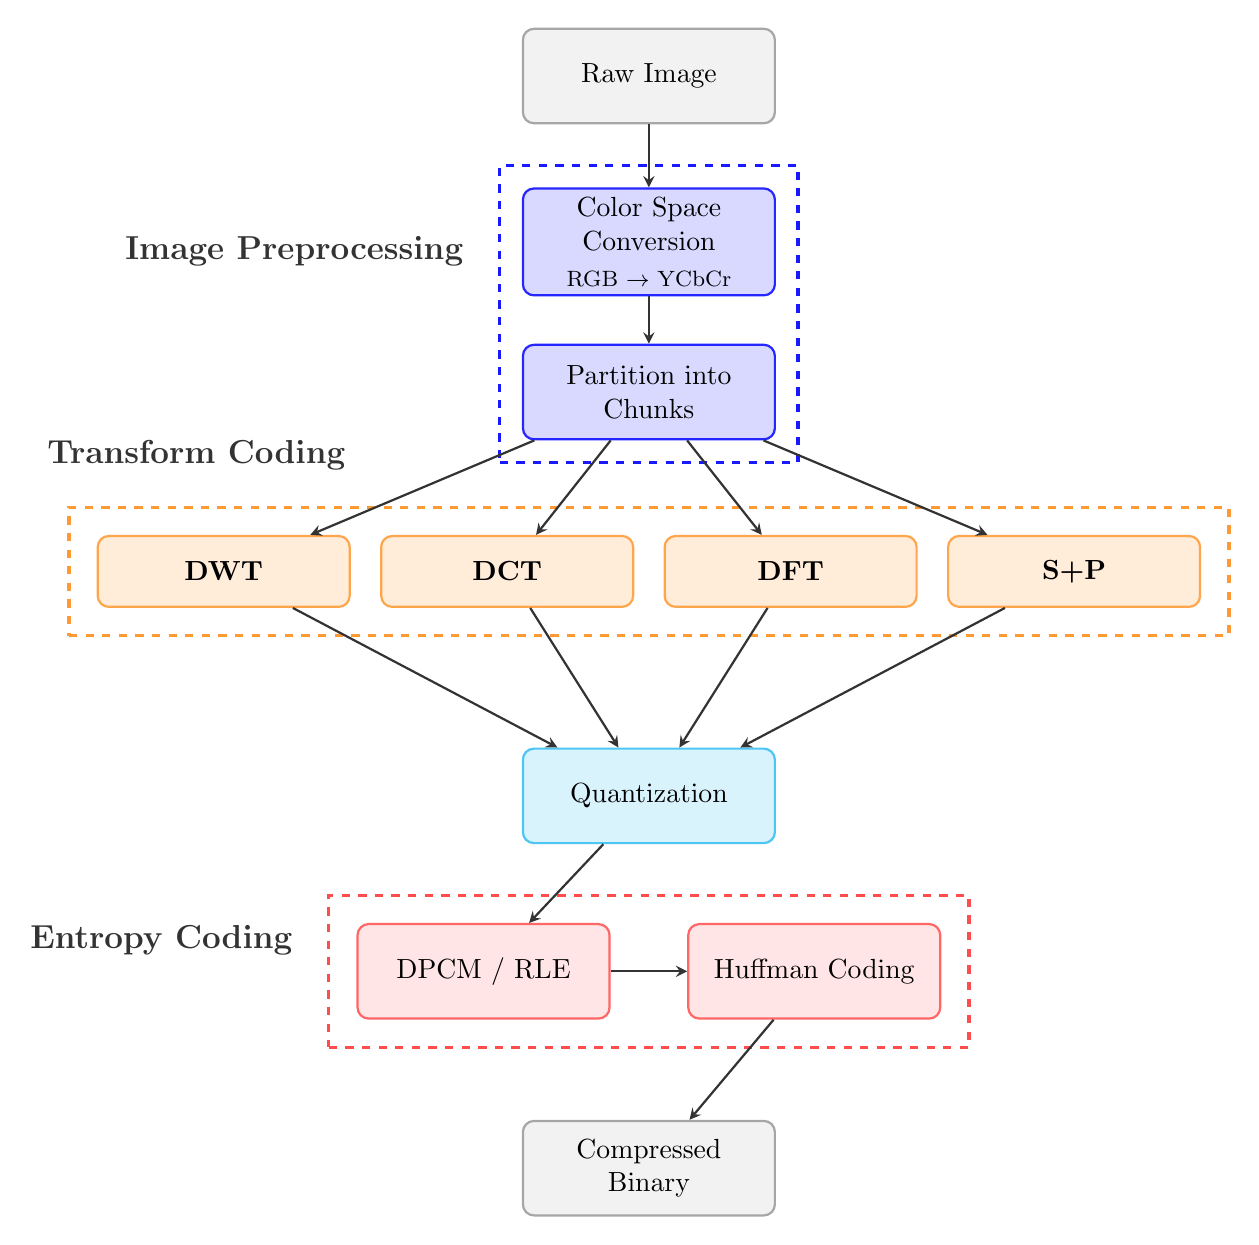
\begin{tikzpicture}[
  input/.style={rectangle,rounded corners=4pt,draw=gray!70,fill=gray!10,thick,
                minimum width=3.2cm,minimum height=1.2cm,align=center},
  process/.style={rectangle,rounded corners=4pt,draw=blue!85,fill=blue!15,thick,
                  minimum width=3.2cm,minimum height=1.2cm,align=center},
  transform/.style={rectangle,rounded corners=4pt,draw=orange!70,fill=orange!15,thick,
                    minimum width=3.2cm,minimum height=0.9cm,align=center,font=\bfseries},
  quant/.style={rectangle,rounded corners=4pt,draw=cyan!70,fill=cyan!15,thick,
                minimum width=3.2cm,minimum height=1.2cm,align=center},
  entropy/.style={rectangle,rounded corners=4pt,draw=red!60,fill=red!10,thick,
                  minimum width=3.2cm,minimum height=1.2cm,align=center},
  output/.style={rectangle,rounded corners=4pt,draw=gray!70,fill=gray!10,thick,
                 minimum width=3.2cm,minimum height=1.2cm,align=center},
  arrow/.style={->,>=stealth,thick,black!80},
  sectionlabel/.style={font=\small\bfseries,black!80,fill=white,inner sep=1pt}
]

% ===== INPUT =====
\node[input] (input) {Raw Image};

% ===== PREPROCESSING =====
\node[process,below=8mm of input] (colorspace) {Color Space\\Conversion\\[1pt]\footnotesize RGB $\rightarrow$ YCbCr};
\node[process,below=6mm of colorspace] (chunk) {Partition into\\Chunks};

\node[draw=blue!90,dashed,very thick,fit=(colorspace)(chunk),inner sep=8pt] (pre_box) {};
% title to the LEFT of the dashed box
\node[sectionlabel,anchor=east, font=\large\bfseries] at ($(pre_box.west)+(-4mm,8mm)$) {Image Preprocessing};

\draw[arrow] (input) -- (colorspace);
\draw[arrow] (colorspace) -- (chunk);

% ===== TRANSFORM CODING (parallel) =====
\node[transform,below=12mm of chunk,xshift=-5.4cm] (dwt) {DWT};
\node[transform,below=12mm of chunk,xshift=-1.8cm] (dct) {DCT};
\node[transform,below=12mm of chunk,xshift=+1.8cm]  (dft) {DFT};
\node[transform,below=12mm of chunk,xshift=+5.4cm] (sp) {S+P};

\node[draw=orange!80,dashed,very thick,fit=(dwt)(dct)(dft)(sp),inner sep=10pt] (tf_box) {};
% title to the LEFT of the dashed box
\node[sectionlabel,anchor=east, font=\large\bfseries] at ($(chunk.west)+(-22mm,-8mm)$) {Transform Coding};

\foreach \t in {dwt,dct,dft,sp} {
  \draw[arrow] (chunk) -- (\t);
}

% ===== QUANTIZATION =====
\node[quant,below=14mm of tf_box] (quant) {Quantization};
\foreach \t in {dwt,dct,dft,sp} {
  \draw[arrow] (\t) -- (quant);
}

% ===== ENTROPY CODING =====
\node[entropy,below=10mm of quant,xshift=-2.1cm] (dpcm) {DPCM / RLE};
\node[entropy,below=10mm of quant,xshift=+2.1cm] (huff) {Huffman Coding};

\node[draw=red!70,dashed,very thick,fit=(dpcm)(huff),inner sep=10pt] (ent_box) {};
% title to the LEFT of the dashed box
\node[sectionlabel,anchor=east, font=\large\bfseries] at ($(ent_box.west)+(-4mm,4mm)$) {Entropy Coding};

% correct arrows through entropy path
\draw[arrow] (quant) -- (dpcm);
\draw[arrow] (dpcm) -- (huff);

% ===== OUTPUT =====
\node[output,below=35mm of quant] (out) {Compressed\\Binary};
\draw[arrow] (huff) -- (out);

% (optional) figure title
% \node[font=\Large\bfseries] at ($(input)+(0,12mm)$) {Image Compression Pipeline};
% We dont need the title for the paper since figures are all already indexed and named

\end{tikzpicture}
\end{document}

    }
    \caption{Image compression pipeline.}
\end{figure}

We begin with a raw RGB image. Because RGB channels are highly correlated, we first convert the image into YCbCr, where luminance (Y) is separated from chrominance (Cb, Cr). This step concentrates most visually important information into a single channel, making subsequent compression more effective. Next, the image is partitioned into blocks as per the specific transform (e.g., 8×8 for DCT/DFT, full-image tiles for Haar and S+P). 

Then, the transform stage is the core of our investigation. Here we substitute one of four transforms (DCT, DFT, Haar, or S+P), while keeping all later steps unchanged, with the exception of routine subband-aware quantization for S+P (described in Section \ref{methodsec:quant}). Each transform maps spatial pixel values into a domain where redundancy is more explicit: DCT and DFT concentrate energy into low-frequency coefficients; Haar and S+P build a multiresolution decomposition. All transforms produce a set of coefficients organized into subbands or frequency components.

These coefficients then undergo quantization, the primary source of loss in the pipeline. Quantization is a nonlinear operation that partitions the range of possible input values into disjoint intervals and assigns each interval a single representative value (the reconstruction level).
All inputs falling within the same interval are encoded identically, which reduces precision and introduces quantization error. Because transforms ideally decorrelate the signal and push most meaningful information into a small number of coefficients, quantization can discard many small values with limited perceptual impact. This makes quantization the crucial stage where transform quality directly affects rate–distortion behavior.

The quantized coefficients are finally passed into an entropy coding module consisting of prediction (DPCM or linear predictive coding), run-length encoding (RLE) of zeros, and Huffman coding. These operations are lossless and convert long runs of similar or repeated values, introduced by quantization, into compact binary representations.

The output of entropy coding forms the compressed bitstream. Decoding inverts each stage in reverse order. Keeping (virtually) all components except the transform fixed, this pipeline allows us to isolate how each transform influences entropy, compressibility, and reconstruction quality across datasets.
\subsection{Background}
\label{methodsec:background}
% Content for Background Methods subsection
% This file is included in the main conference paper via % Content for Background Methods subsection
% This file is included in the main conference paper via % Content for Background Methods subsection
% This file is included in the main conference paper via \input{Background}

Before diving into the individual transform methods, we first explain what transform coding is and why it helps with compression. The idea is to take the original representation of our image, a 2D array of pixel values, and transform it into a new space with lower entropy. The hope is that the result will be easily compressed by the entropy encoding techniques described in Section \ref{methodsec:entropy}.

We do this by considering some original signal, which we will denote as 
\begin{equation}
        x=\{x_1,x_2,\dots,x_N\}\label{eq:sig}.
\end{equation}
The signal can be thought of as a vector in the vector space $\mathbb{R}^N$. Loosely speaking, a vector space $V$ is any collection of elements where
\begin{enumerate}
    \item For all $a,b\in\mathbb{R}$ and $u,v\in V$, $au+bv\in V$.
    \item There is a unique element $0\in V$ such that for all $v\in V$, $0v=0$ and $v+0=v$.
\end{enumerate}
In other words, it is a space that respects and is closed under the normal operation of addition and multiplication on the real numbers $\mathbb{R}$. Vector spaces have many rich theoretical properties, for which the interested reader can refer to the textbook by Broughton \cite{broughton2009discrete}. We will only cover the most essential properties here. A set of vectors $v_1,v_2,\dots,v_k$ is called \textit{linearly independent} if the only solution to the equation
\begin{equation}
    c_1v_1+c_2v_2+\dotsb+c_kv_k=0\label{eq:lin_ind}
\end{equation}
is that $c_i=0$ for $i=1,2,\dots,k$. A set of linearly independent vectors $v_1,v_2,\dots,v_N$ is called a \textit{basis} if for any vector $u\in V$, there exists numbers $c_1,c_2,\dots,c_N$ such that
\begin{equation}
    u=\sum_{i=1}^{N}c_iv_i.
\end{equation}
In other words, every member of the vector space can be represented as some weighted sum of vectors in a basis. These weights $c_1,c_2,\dots,c_N$ are called the coefficients. Fig. \ref{fig:2dbasis} illustrates this with one of the simplest examples $\mathbb{R}^2$, where the vectors $\langle0,1\rangle$ and $\langle1,0\rangle$ form a basis. In this example, we get the equation $v=3i+2j$ where $3$ and $2$ are our coefficients.
\begin{figure}
    \centering
    \includestandalone[width=0.6\linewidth]{methods/Fourierdiagrams/BasisExample}
    \caption{The vectors $\vec{i}$ and $\vec{j}$ form a 2D basis of $\mathbb{R}^2$}
    \label{fig:2dbasis}
\end{figure}
Notably, for any given vector space there are many possible bases. The transform algorithms described in this section are all effectively a \textit{change of basis}, where the new, transformed signal is denoted
\begin{equation}
    X=\{X_1,X_2,\dots,X_N\}.\label{eq:tsig}
\end{equation}
These new values can be thought of as the coordinates for the signal in the new transformed space. By cleverly choosing a basis, the hope is that more information of the original data is encoded in fewer of the new coefficients.

Applying this to images specifically, if we represent our image as a 2D array of pixels, the resulting transformed image can be acquired by applying the transform to each row and column, as demonstrated in Fig. \ref{fig:2dtransform}.
\begin{figure}
    \centering
    \includestandalone[width=1.0\linewidth]{methods/Fourierdiagrams/2DTransform}
    \caption{Applying a transform to an image}
    \label{fig:2dtransform}
\end{figure}

Before diving into the individual transform methods, we first explain what transform coding is and why it helps with compression. The idea is to take the original representation of our image, a 2D array of pixel values, and transform it into a new space with lower entropy. The hope is that the result will be easily compressed by the entropy encoding techniques described in Section \ref{methodsec:entropy}.

We do this by considering some original signal, which we will denote as 
\begin{equation}
        x=\{x_1,x_2,\dots,x_N\}\label{eq:sig}.
\end{equation}
The signal can be thought of as a vector in the vector space $\mathbb{R}^N$. Loosely speaking, a vector space $V$ is any collection of elements where
\begin{enumerate}
    \item For all $a,b\in\mathbb{R}$ and $u,v\in V$, $au+bv\in V$.
    \item There is a unique element $0\in V$ such that for all $v\in V$, $0v=0$ and $v+0=v$.
\end{enumerate}
In other words, it is a space that respects and is closed under the normal operation of addition and multiplication on the real numbers $\mathbb{R}$. Vector spaces have many rich theoretical properties, for which the interested reader can refer to the textbook by Broughton \cite{broughton2009discrete}. We will only cover the most essential properties here. A set of vectors $v_1,v_2,\dots,v_k$ is called \textit{linearly independent} if the only solution to the equation
\begin{equation}
    c_1v_1+c_2v_2+\dotsb+c_kv_k=0\label{eq:lin_ind}
\end{equation}
is that $c_i=0$ for $i=1,2,\dots,k$. A set of linearly independent vectors $v_1,v_2,\dots,v_N$ is called a \textit{basis} if for any vector $u\in V$, there exists numbers $c_1,c_2,\dots,c_N$ such that
\begin{equation}
    u=\sum_{i=1}^{N}c_iv_i.
\end{equation}
In other words, every member of the vector space can be represented as some weighted sum of vectors in a basis. These weights $c_1,c_2,\dots,c_N$ are called the coefficients. Fig. \ref{fig:2dbasis} illustrates this with one of the simplest examples $\mathbb{R}^2$, where the vectors $\langle0,1\rangle$ and $\langle1,0\rangle$ form a basis. In this example, we get the equation $v=3i+2j$ where $3$ and $2$ are our coefficients.
\begin{figure}
    \centering
    \includestandalone[width=0.6\linewidth]{methods/Fourierdiagrams/BasisExample}
    \caption{The vectors $\vec{i}$ and $\vec{j}$ form a 2D basis of $\mathbb{R}^2$}
    \label{fig:2dbasis}
\end{figure}
Notably, for any given vector space there are many possible bases. The transform algorithms described in this section are all effectively a \textit{change of basis}, where the new, transformed signal is denoted
\begin{equation}
    X=\{X_1,X_2,\dots,X_N\}.\label{eq:tsig}
\end{equation}
These new values can be thought of as the coordinates for the signal in the new transformed space. By cleverly choosing a basis, the hope is that more information of the original data is encoded in fewer of the new coefficients.

Applying this to images specifically, if we represent our image as a 2D array of pixels, the resulting transformed image can be acquired by applying the transform to each row and column, as demonstrated in Fig. \ref{fig:2dtransform}.
\begin{figure}
    \centering
    \includestandalone[width=1.0\linewidth]{methods/Fourierdiagrams/2DTransform}
    \caption{Applying a transform to an image}
    \label{fig:2dtransform}
\end{figure}

Before diving into the individual transform methods, we first explain what transform coding is and why it helps with compression. The idea is to take the original representation of our image, a 2D array of pixel values, and transform it into a new space with lower entropy. The hope is that the result will be easily compressed by the entropy encoding techniques described in Section \ref{methodsec:entropy}.

We do this by considering some original signal, which we will denote as 
\begin{equation}
        x=\{x_1,x_2,\dots,x_N\}\label{eq:sig}.
\end{equation}
The signal can be thought of as a vector in the vector space $\mathbb{R}^N$. Loosely speaking, a vector space $V$ is any collection of elements where
\begin{enumerate}
    \item For all $a,b\in\mathbb{R}$ and $u,v\in V$, $au+bv\in V$.
    \item There is a unique element $0\in V$ such that for all $v\in V$, $0v=0$ and $v+0=v$.
\end{enumerate}
In other words, it is a space that respects and is closed under the normal operation of addition and multiplication on the real numbers $\mathbb{R}$. Vector spaces have many rich theoretical properties, for which the interested reader can refer to the textbook by Broughton \cite{broughton2009discrete}. We will only cover the most essential properties here. A set of vectors $v_1,v_2,\dots,v_k$ is called \textit{linearly independent} if the only solution to the equation
\begin{equation}
    c_1v_1+c_2v_2+\dotsb+c_kv_k=0\label{eq:lin_ind}
\end{equation}
is that $c_i=0$ for $i=1,2,\dots,k$. A set of linearly independent vectors $v_1,v_2,\dots,v_N$ is called a \textit{basis} if for any vector $u\in V$, there exists numbers $c_1,c_2,\dots,c_N$ such that
\begin{equation}
    u=\sum_{i=1}^{N}c_iv_i.
\end{equation}
In other words, every member of the vector space can be represented as some weighted sum of vectors in a basis. These weights $c_1,c_2,\dots,c_N$ are called the coefficients. Fig. \ref{fig:2dbasis} illustrates this with one of the simplest examples $\mathbb{R}^2$, where the vectors $\langle0,1\rangle$ and $\langle1,0\rangle$ form a basis. In this example, we get the equation $v=3i+2j$ where $3$ and $2$ are our coefficients.
\begin{figure}
    \centering
    \includestandalone[width=0.6\linewidth]{methods/Fourierdiagrams/BasisExample}
    \caption{The vectors $\vec{i}$ and $\vec{j}$ form a 2D basis of $\mathbb{R}^2$}
    \label{fig:2dbasis}
\end{figure}
Notably, for any given vector space there are many possible bases. The transform algorithms described in this section are all effectively a \textit{change of basis}, where the new, transformed signal is denoted
\begin{equation}
    X=\{X_1,X_2,\dots,X_N\}.\label{eq:tsig}
\end{equation}
These new values can be thought of as the coordinates for the signal in the new transformed space. By cleverly choosing a basis, the hope is that more information of the original data is encoded in fewer of the new coefficients.

Applying this to images specifically, if we represent our image as a 2D array of pixels, the resulting transformed image can be acquired by applying the transform to each row and column, as demonstrated in Fig. \ref{fig:2dtransform}.
\begin{figure}
    \centering
    \includestandalone[width=1.0\linewidth]{methods/Fourierdiagrams/2DTransform}
    \caption{Applying a transform to an image}
    \label{fig:2dtransform}
\end{figure}
\subsection{Discrete Wavelet Transform}
Luca
% Content for DWT Methods subsection
% This file is included in the main conference paper via % Content for DWT Methods subsection
% This file is included in the main conference paper via % Content for DWT Methods subsection
% This file is included in the main conference paper via \input{DWTMethods}

The Discrete Wavelet Transform (DWT) is a powerful transform coding technique that decomposes signals into a hierarchy of resolution levels, making it particularly well-suited for image compression. In this work we focus on the Haar wavelet, which is the simplest in the family of wavelets used for this transform. For now on we consider an image as a 1D signal, we later discuss how to convert it to 2D.

\subsubsection{One Dimensional Haar Wavelet Transform in Practice}

Consider a 1D signal with $2^k$ values: $$ \{x_1, x_2, \dots, x_{2^k}\}$$ A naive approach to compression might be to store only the average of adjacent values, resulting in the compressed signal $$A_{k-1} = \{(x_1 + x_2) / 2, (x_3 + x_4) / 2, \dots, (x_{2^k-1} + x_{2^k})/2\}$$ Note that this approach clearly loses information. To enable perfect reconstruction of the original signal, we must also preserve the difference between adjacent values: $$D_{k-1} = \{x_1 - (x_1 + x_2) / 2, x_3 - (x_3 + x_4) / 2, \dots\}$$
Note that the difference of $x_i$ the the mean is completely symmetric to the difference of $x_{i+1}$ to the mean, so we only need to store one detail coefficient. This simple idea is the core of the Haar wavelet transform.

We can apply this operation once and we get a set of $2^k/2$ average coefficients and $2^k/2$ detail coefficients. We can keep applying the operation recursively to the average coefficients until we reach only one pixel of average coefficient. Table~\ref{tab:haar_decomposition} illustrates this process for an 8-pixel signal.

Figure~\ref{fig:haar_decomposition} visualizes this decomposition process, showing the signal (blue) and wavelets (red) at each resolution level. The blue curves represent the averaged signals at decreasing resolutions, while the red curves capture the detail coefficients (differences) that must be preserved for perfect reconstruction.

\begin{table}[h]
  \centering
  \caption{Haar decomposition example for an 8-pixel signal}
  \label{tab:haar_decomposition}
  \begin{tabular}{c c c}
    \toprule
    \textbf{Resolution} & \textbf{Averages} & \textbf{Details} \\
    \midrule
    8 & $[5, \; 8, \; 9, \; 7, \; 4, \; 2, \; 1, \; 3]$ & --- \\
    4 & $[6.5, \; 8, \; 3, \; 2]$ & $[-1.5, \; 1, \; 1, \; -1]$ \\
    2 & $[7.25, \; 2.5]$ & $[-0.75, \; 0.5]$ \\
    1 & $[4.875]$ & $[2.375]$ \\
    \bottomrule
  \end{tabular}
\end{table}

\begin{figure}[ht]
  \centering
  \input{methods/DWTdiagrams/haar_decomposition}
  \caption{Haar wavelet decomposition showing signal (blue) and wavelets (red) at each resolution level.}
  \label{fig:haar_decomposition}
\end{figure}

Note that for a given level we can perfectly reconstruct the previous level's average coefficients from the combination of the average coefficient and detail coefficients, so all we need to store in a compression is the set of all detail coefficients and the very last average.

\subsubsection{Theoretical Foundation for Haar Wavelet Transform}

The Haar wavelet transform is founded on a set of nested vector spaces $V^j$ representing piecewise-constant functions at different resolutions, where $V^0 \subset V^1 \subset V^2 \subset \dots$. This nested structure enables a change of basis from the natural basis of scaling functions in $V^{j+1}$ to a basis consisting of the scaling functions from the lower-resolution space $V^j$ together with the wavelet basis functions from the orthogonal complement space $W^j$. The scaling functions provide the coarse approximation, while the wavelets capture the detail information needed for perfect reconstruction. Figure~\ref{fig:basis_functions} visualizes the scaling functions and Haar wavelets for different resolution levels.

\begin{figure*}[hbt]
  \centering
  \begin{minipage}{\textwidth}
    \centering
    \input{methods/DWTdiagrams/scaling_functions}
    \subcaption{Scaling functions (basis) for $V^3$: eight piecewise constant functions.}
    \label{fig:scaling_functions}
  \end{minipage}
  \vspace{0.5cm}
  \begin{minipage}{\textwidth}
    \centering
    \input{methods/DWTdiagrams/wavelet_basis}
    \subcaption{Basis for $V^2$ (blue) and Haar wavelets basis for $W^2$ (red).}
    \label{fig:wavelet_basis}
  \end{minipage}
  \caption{Haar basis: scaling functions for $V^3$ and scaling functions and wavelets for $V^2$ and $W^2$.}
  \label{fig:basis_functions}
\end{figure*}

A detailed mathematical exposition of the vector space structure, scaling functions, inner products, orthogonality, and the Haar wavelet basis functions is provided in Appendix \ref{apx:haartheory}.




\subsubsection{Two-Dimensional Haar Wavelet Transform}

The 2D Haar wavelet transform generalizes the 1D "averaging and differencing" filter bank to 2D by alternating between operations on rows and columns at each level of the hierarchy.

\paragraph{The Decomposition Algorithm}

The algorithm proceeds recursively as follows:

\begin{enumerate}
\item \textbf{Row Step:} First, perform one step of horizontal pairwise averaging and differencing on the pixel values in each row of the image. This splits the image horizontally into averages (left) and details (right).

\item \textbf{Column Step:} Next, apply vertical pairwise averaging and differencing to each column of the result from the Row Step.
\begin{itemize}
\item This creates four distinct quadrants of coefficients:
\begin{itemize}
\item \textbf{Top-Left:} Averages of averages (coarse approximation).
\item \textbf{Top-Right:} Averages of horizontal details.
\item \textbf{Bottom-Left:} Vertical details of horizontal averages.
\item \textbf{Bottom-Right:} Vertical details of horizontal details (diagonal details).
\end{itemize}
\end{itemize}

\item \textbf{Recursion:} To complete the transformation, repeat this process recursively \textit{only} on the quadrant containing the averages in both directions (the top-left quadrant).
\end{enumerate}

Figure~\ref{fig:encoded_visualization} visualizes this 2D Haar transform decomposition process, showing how an image is decomposed into four quadrants at each level.

\begin{figure}[ht]
  \centering
  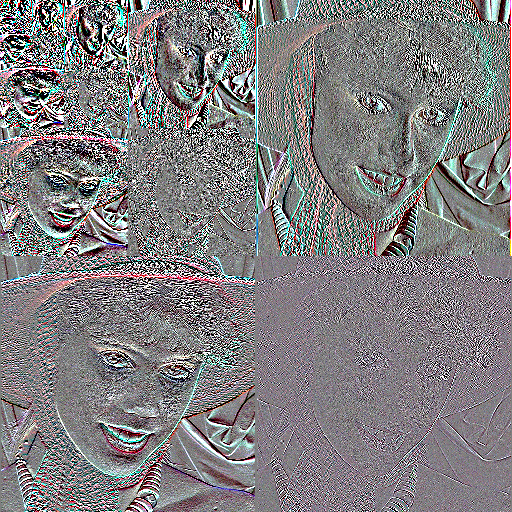
\includegraphics[width=0.3\textwidth]{methods/DWTdiagrams/encodedVisualization.png}
  \caption{Visualization of a 2D Haar transform showing the decomposition of an image}
  \label{fig:encoded_visualization}
\end{figure}




\subsubsection{Compression Properties}

The Haar wavelet transform is particularly effective for image compression because it naturally concentrates energy in the low-resolution approximation coefficients. The detail coefficients (wavelets) typically have smaller magnitudes and can be more aggressively quantized or discarded in lossy compression scenarios. This energy compaction property, combined with the transform's computational efficiency makes the Haar wavelet an attractive choice for practical image compression systems.



The Discrete Wavelet Transform (DWT) is a powerful transform coding technique that decomposes signals into a hierarchy of resolution levels, making it particularly well-suited for image compression. In this work we focus on the Haar wavelet, which is the simplest in the family of wavelets used for this transform. For now on we consider an image as a 1D signal, we later discuss how to convert it to 2D.

\subsubsection{One Dimensional Haar Wavelet Transform in Practice}

Consider a 1D signal with $2^k$ values: $$ \{x_1, x_2, \dots, x_{2^k}\}$$ A naive approach to compression might be to store only the average of adjacent values, resulting in the compressed signal $$A_{k-1} = \{(x_1 + x_2) / 2, (x_3 + x_4) / 2, \dots, (x_{2^k-1} + x_{2^k})/2\}$$ Note that this approach clearly loses information. To enable perfect reconstruction of the original signal, we must also preserve the difference between adjacent values: $$D_{k-1} = \{x_1 - (x_1 + x_2) / 2, x_3 - (x_3 + x_4) / 2, \dots\}$$
Note that the difference of $x_i$ the the mean is completely symmetric to the difference of $x_{i+1}$ to the mean, so we only need to store one detail coefficient. This simple idea is the core of the Haar wavelet transform.

We can apply this operation once and we get a set of $2^k/2$ average coefficients and $2^k/2$ detail coefficients. We can keep applying the operation recursively to the average coefficients until we reach only one pixel of average coefficient. Table~\ref{tab:haar_decomposition} illustrates this process for an 8-pixel signal.

Figure~\ref{fig:haar_decomposition} visualizes this decomposition process, showing the signal (blue) and wavelets (red) at each resolution level. The blue curves represent the averaged signals at decreasing resolutions, while the red curves capture the detail coefficients (differences) that must be preserved for perfect reconstruction.

\begin{table}[h]
  \centering
  \caption{Haar decomposition example for an 8-pixel signal}
  \label{tab:haar_decomposition}
  \begin{tabular}{c c c}
    \toprule
    \textbf{Resolution} & \textbf{Averages} & \textbf{Details} \\
    \midrule
    8 & $[5, \; 8, \; 9, \; 7, \; 4, \; 2, \; 1, \; 3]$ & --- \\
    4 & $[6.5, \; 8, \; 3, \; 2]$ & $[-1.5, \; 1, \; 1, \; -1]$ \\
    2 & $[7.25, \; 2.5]$ & $[-0.75, \; 0.5]$ \\
    1 & $[4.875]$ & $[2.375]$ \\
    \bottomrule
  \end{tabular}
\end{table}

\begin{figure}[ht]
  \centering
  % Haar wavelet decomposition diagram showing signal and wavelets at each resolution level
% Arranged in a 2x2 grid to fit in a single column
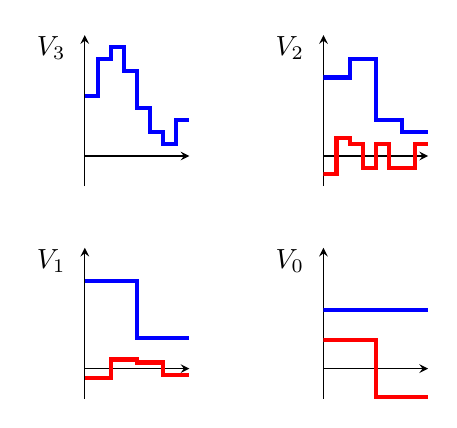
\begin{tikzpicture}
  % Top row: Resolution 8 (V_3) - top left
  \begin{axis}[
    at={(0.13\textwidth,4.5cm)},
    width=0.24\textwidth,
    height=3.5cm,
    xmin=0, xmax=1,
    ymin=-2.5, ymax=10,
    ytick=\empty,
    xtick=\empty,
    axis x line=middle,
    axis y line=center,
  ]
    \addplot[const plot, line width=1.5pt, color=blue] coordinates {
      (0,5) (0.125,5) (0.125,8) (0.25,8) (0.25,9) (0.375,9) (0.375,7) (0.5,7) (0.5,4) (0.625,4) (0.625,2) (0.75,2) (0.75,1) (0.875,1) (0.875,3) (1,3)
    };
  \end{axis}
  \node[anchor=east] at (0.12\textwidth, 6.25cm) {$V_3$};
  
  % Top row: Resolution 4 (V_2) - top right
  \begin{axis}[
    at={(0.38\textwidth,4.5cm)},
    width=0.24\textwidth,
    height=3.5cm,
    xmin=0, xmax=1,
    ymin=-2.5, ymax=10,
    ytick=\empty,
    xtick=\empty,
    axis x line=middle,
    axis y line=center,
  ]
    \addplot[const plot, line width=1.5pt, color=blue] coordinates {
      (0,6.5) (0.25,6.5) (0.25,8) (0.5,8) (0.5,3) (0.75,3) (0.75,2) (1,2)
    };
    \addplot[const plot, line width=1.5pt, color=red] coordinates {
      (0,-1.5) (0.125,-1.5) (0.125,1.5) (0.25,1.5) (0.25,1) (0.375,1) (0.375,-1) (0.5,-1) (0.5,1) (0.625,1) (0.625,-1) (0.75,-1) (0.75,-1) (0.875,-1) (0.875,1) (1,1)
    };
  \end{axis}
  \node[anchor=east] at (0.37\textwidth, 6.25cm) {$V_2$};

  % Bottom row: Resolution 2 (V_1) - bottom left
  \begin{axis}[
    at={(0.13\textwidth,1.8cm)},
    width=0.24\textwidth,
    height=3.5cm,
    xmin=0, xmax=1,
    ymin=-2.5, ymax=10,
    ytick=\empty,
    xtick=\empty,
    axis x line=middle,
    axis y line=center,
  ]
    \addplot[const plot, line width=1.5pt, color=blue] coordinates {
      (0,7.25) (0.5,7.25) (0.5,2.5) (1,2.5)
    };
    \addplot[const plot, line width=1.5pt, color=red] coordinates {
      (0,-0.75) (0.25,-0.75) (0.25,0.75) (0.5,0.75) (0.5,0.5) (0.75,0.5) (0.75,-0.5) (1,-0.5)
    };
  \end{axis}
  \node[anchor=east] at (0.12\textwidth, 3.55cm) {$V_1$};
  
  % Bottom row: Resolution 1 (V_0) - bottom right
  \begin{axis}[
    at={(0.38\textwidth,1.8cm)},
    width=0.24\textwidth,
    height=3.5cm,
    xmin=0, xmax=1,
    ymin=-2.5, ymax=10,
    ytick=\empty,
    xtick=\empty,
    axis x line=middle,
    axis y line=center,
  ]
    \addplot[const plot, line width=1.5pt, color=blue] coordinates {
      (0,4.875) (1,4.875)
    };
    \addplot[const plot, line width=1.5pt, color=red] coordinates {
      (0,2.375) (0.5,2.375) (0.5,-2.375) (1,-2.375)
    };
  \end{axis}
  \node[anchor=east] at (0.37\textwidth, 3.55cm) {$V_0$};

\end{tikzpicture}


  \caption{Haar wavelet decomposition showing signal (blue) and wavelets (red) at each resolution level.}
  \label{fig:haar_decomposition}
\end{figure}

Note that for a given level we can perfectly reconstruct the previous level's average coefficients from the combination of the average coefficient and detail coefficients, so all we need to store in a compression is the set of all detail coefficients and the very last average.

\subsubsection{Theoretical Foundation for Haar Wavelet Transform}

The Haar wavelet transform is founded on a set of nested vector spaces $V^j$ representing piecewise-constant functions at different resolutions, where $V^0 \subset V^1 \subset V^2 \subset \dots$. This nested structure enables a change of basis from the natural basis of scaling functions in $V^{j+1}$ to a basis consisting of the scaling functions from the lower-resolution space $V^j$ together with the wavelet basis functions from the orthogonal complement space $W^j$. The scaling functions provide the coarse approximation, while the wavelets capture the detail information needed for perfect reconstruction. Figure~\ref{fig:basis_functions} visualizes the scaling functions and Haar wavelets for different resolution levels.

\begin{figure*}[hbt]
  \centering
  \begin{minipage}{\textwidth}
    \centering
    % Scaling functions (basis) for V_3: eight piecewise constant functions
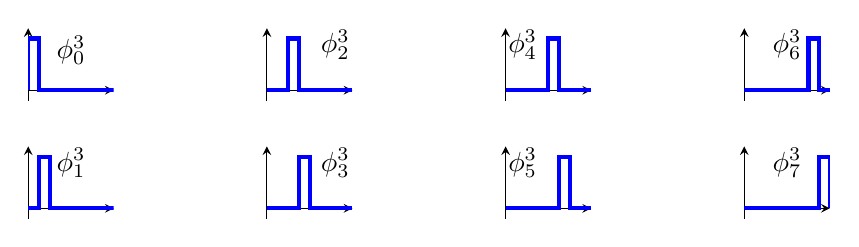
\begin{tikzpicture}
  % Column 1: Scaling functions 1 and 2
  % Scaling function 1: [0, 1/8)
  \begin{axis}[
    at={(0,0)},
    width=0.22\textwidth,
    height=2.5cm,
    xmin=0, xmax=1,
    ymin=-0.2, ymax=1.2,
    ytick=\empty,
    xtick=\empty,
    axis x line=middle,
    axis y line=center,
  ]
    \addplot[const plot, line width=1.5pt, color=blue] coordinates {
      (0,0) (0,1) (0.125,1) (0.125,0) (1,0)
    };
    \node[above] at (0.5, 0.3) {$\phi_0^3$};
  \end{axis}
  % Scaling function 2: [1/8, 1/4)
  \begin{axis}[
    at={(0,-1.5cm)},
    width=0.22\textwidth,
    height=2.5cm,
    xmin=0, xmax=1,
    ymin=-0.2, ymax=1.2,
    ytick=\empty,
    xtick=\empty,
    axis x line=middle,
    axis y line=center,
  ]
    \addplot[const plot, line width=1.5pt, color=blue] coordinates {
      (0,0) (0.125,0) (0.125,1) (0.25,1) (0.25,0) (1,0)
    };
    \node[above] at (0.5, 0.4) {$\phi_1^3$};
  \end{axis}
  
  % Column 2: Scaling functions 3 and 4
  % Scaling function 3: [1/4, 3/8)
  \begin{axis}[
    at={(0.25\textwidth,0)},
    width=0.22\textwidth,
    height=2.5cm,
    xmin=0, xmax=1,
    ymin=-0.2, ymax=1.2,
    ytick=\empty,
    xtick=\empty,
    axis x line=middle,
    axis y line=center,
  ]
    \addplot[const plot, line width=1.5pt, color=blue] coordinates {
      (0,0) (0.25,0) (0.25,1) (0.375,1) (0.375,0) (1,0)
    };
    \node[above] at (0.8, 0.4) {$\phi_2^3$};
  \end{axis}
  % Scaling function 4: [3/8, 1/2)
  \begin{axis}[
    at={(0.25\textwidth,-1.5cm)},
    width=0.22\textwidth,
    height=2.5cm,
    xmin=0, xmax=1,
    ymin=-0.2, ymax=1.2,
    ytick=\empty,
    xtick=\empty,
    axis x line=middle,
    axis y line=center,
  ]
    \addplot[const plot, line width=1.5pt, color=blue] coordinates {
      (0,0) (0.375,0) (0.375,1) (0.5,1) (0.5,0) (1,0)
    };
    \node[above] at (0.8, 0.4) {$\phi_3^3$};
  \end{axis}
  
  % Column 3: Scaling functions 5 and 6
  % Scaling function 5: [1/2, 5/8)
  \begin{axis}[
    at={(0.5\textwidth,0)},
    width=0.22\textwidth,
    height=2.5cm,
    xmin=0, xmax=1,
    ymin=-0.2, ymax=1.2,
    ytick=\empty,
    xtick=\empty,
    axis x line=middle,
    axis y line=center,
  ]
    \addplot[const plot, line width=1.5pt, color=blue] coordinates {
      (0,0) (0.5,0) (0.5,1) (0.625,1) (0.625,0) (1,0)
    };
    \node[above] at (0.2, 0.4) {$\phi_4^3$};
  \end{axis}
  % Scaling function 6: [5/8, 3/4)
  \begin{axis}[
    at={(0.5\textwidth,-1.5cm)},
    width=0.22\textwidth,
    height=2.5cm,
    xmin=0, xmax=1,
    ymin=-0.2, ymax=1.2,
    ytick=\empty,
    xtick=\empty,
    axis x line=middle,
    axis y line=center,
  ]
    \addplot[const plot, line width=1.5pt, color=blue] coordinates {
      (0,0) (0.625,0) (0.625,1) (0.75,1) (0.75,0) (1,0)
    };
    \node[above] at (0.2, 0.4) {$\phi_5^3$};
  \end{axis}
  
  % Column 4: Scaling functions 7 and 8
  % Scaling function 7: [3/4, 7/8)
  \begin{axis}[
    at={(0.75\textwidth,0)},
    width=0.22\textwidth,
    height=2.5cm,
    xmin=0, xmax=1,
    ymin=-0.2, ymax=1.2,
    ytick=\empty,
    xtick=\empty,
    axis x line=middle,
    axis y line=center,
  ]
    \addplot[const plot, line width=1.5pt, color=blue] coordinates {
      (0,0) (0.75,0) (0.75,1) (0.875,1) (0.875,0) (1,0)
    };
    \node[above] at (0.5, 0.4) {$\phi_6^3$};
  \end{axis}
  % Scaling function 8: [7/8, 1)
  \begin{axis}[
    at={(0.75\textwidth,-1.5cm)},
    width=0.22\textwidth,
    height=2.5cm,
    xmin=0, xmax=1,
    ymin=-0.2, ymax=1.2,
    ytick=\empty,
    xtick=\empty,
    axis x line=middle,
    axis y line=center,
  ]
    \addplot[const plot, line width=1.5pt, color=blue] coordinates {
      (0,0) (0.875,0) (0.875,1) (1,1) (1,0)
    };
    \node[above] at (0.5, 0.4) {$\phi_7^3$};
  \end{axis}
\end{tikzpicture}


    \subcaption{Scaling functions (basis) for $V^3$: eight piecewise constant functions.}
    \label{fig:scaling_functions}
  \end{minipage}
  \vspace{0.5cm}
  \begin{minipage}{\textwidth}
    \centering
    % Basis for V_2 (blue) and Haar wavelets basis for W_2 (red)
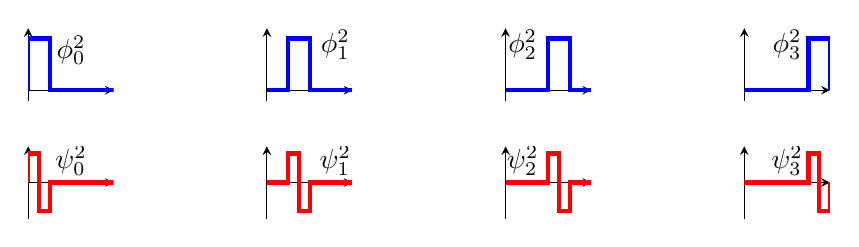
\begin{tikzpicture}
  % V_2 Scaling functions (row above)
  % Scaling function 1: [0, 1/4)
  \begin{axis}[
    at={(0,1.5cm)},
    width=0.22\textwidth,
    height=2.5cm,
    xmin=0, xmax=1,
    ymin=-0.2, ymax=1.2,
    ytick=\empty,
    xtick=\empty,
    axis x line=middle,
    axis y line=center,
  ]
    \addplot[const plot, line width=1.5pt, color=blue] coordinates {
      (0,0) (0,1) (0.25,1) (0.25,0) (1,0)
    };
    \node[above] at (0.5, 0.3) {$\phi_0^2$};
  \end{axis}
  % Scaling function 2: [1/4, 1/2)
  \begin{axis}[
    at={(0.25\textwidth,1.5cm)},
    width=0.22\textwidth,
    height=2.5cm,
    xmin=0, xmax=1,
    ymin=-0.2, ymax=1.2,
    ytick=\empty,
    xtick=\empty,
    axis x line=middle,
    axis y line=center,
  ]
    \addplot[const plot, line width=1.5pt, color=blue] coordinates {
      (0,0) (0.25,0) (0.25,1) (0.5,1) (0.5,0) (1,0)
    };
    \node[above] at (0.8, 0.4) {$\phi_1^2$};
  \end{axis}
  % Scaling function 3: [1/2, 3/4)
  \begin{axis}[
    at={(0.5\textwidth,1.5cm)},
    width=0.22\textwidth,
    height=2.5cm,
    xmin=0, xmax=1,
    ymin=-0.2, ymax=1.2,
    ytick=\empty,
    xtick=\empty,
    axis x line=middle,
    axis y line=center,
  ]
    \addplot[const plot, line width=1.5pt, color=blue] coordinates {
      (0,0) (0.5,0) (0.5,1) (0.75,1) (0.75,0) (1,0)
    };
    \node[above] at (0.2, 0.4) {$\phi_2^2$};
  \end{axis}
  % Scaling function 4: [3/4, 1)
  \begin{axis}[
    at={(0.75\textwidth,1.5cm)},
    width=0.22\textwidth,
    height=2.5cm,
    xmin=0, xmax=1,
    ymin=-0.2, ymax=1.2,
    ytick=\empty,
    xtick=\empty,
    axis x line=middle,
    axis y line=center,
  ]
    \addplot[const plot, line width=1.5pt, color=blue] coordinates {
      (0,0) (0.75,0) (0.75,1) (1,1) (1,0)
    };
    \node[above] at (0.5, 0.4) {$\phi_3^2$};
  \end{axis}
  
  % Wavelet level 2, first: [0, 1/8) vs [1/8, 1/4)
  \begin{axis}[
    at={(0,0)},
    width=0.22\textwidth,
    height=2.5cm,
    xmin=0, xmax=1,
    ymin=-2.5, ymax=2.5,
    ytick=\empty,
    xtick=\empty,
    axis x line=middle,
    axis y line=center,
  ]
    \addplot[const plot, line width=1.5pt, color=red] coordinates {
      (0,0) (0,2) (0.125,2) (0.125,-2) (0.25,-2) (0.25,0) (1,0)
    };
    \node[above] at (0.5, -0.2) {$\psi_0^2$};
  \end{axis}
  % Wavelet level 2, second: [1/4, 3/8) vs [3/8, 1/2)
  \begin{axis}[
    at={(0.25\textwidth,0)},
    width=0.22\textwidth,
    height=2.5cm,
    xmin=0, xmax=1,
    ymin=-2.5, ymax=2.5,
    ytick=\empty,
    xtick=\empty,
    axis x line=middle,
    axis y line=center,
  ]
    \addplot[const plot, line width=1.5pt, color=red] coordinates {
      (0,0) (0.25,0) (0.25,2) (0.375,2) (0.375,-2) (0.5,-2) (0.5,0) (1,0)
    };
    \node[above] at (0.8, -0.2) {$\psi_1^2$};
  \end{axis}
  % Wavelet level 2, third: [1/2, 5/8) vs [5/8, 3/4)
  \begin{axis}[
    at={(0.5\textwidth,0)},
    width=0.22\textwidth,
    height=2.5cm,
    xmin=0, xmax=1,
    ymin=-2.5, ymax=2.5,
    ytick=\empty,
    xtick=\empty,
    axis x line=middle,
    axis y line=center,
  ]
    \addplot[const plot, line width=1.5pt, color=red] coordinates {
      (0,0) (0.5,0) (0.5,2) (0.625,2) (0.625,-2) (0.75,-2) (0.75,0) (1,0)
    };
    \node[above] at (0.2, -0.2) {$\psi_2^2$};
  \end{axis}
  % Wavelet level 2, fourth: [3/4, 7/8) vs [7/8, 1)
  \begin{axis}[
    at={(0.75\textwidth,0)},
    width=0.22\textwidth,
    height=2.5cm,
    xmin=0, xmax=1,
    ymin=-2.5, ymax=2.5,
    ytick=\empty,
    xtick=\empty,
    axis x line=middle,
    axis y line=center,
  ]
    \addplot[const plot, line width=1.5pt, color=red] coordinates {
      (0,0) (0.75,0) (0.75,2) (0.875,2) (0.875,-2) (1,-2) (1,0)
    };
    \node[above] at (0.5, -0.2) {$\psi_3^2$};
  \end{axis}
\end{tikzpicture}


    \subcaption{Basis for $V^2$ (blue) and Haar wavelets basis for $W^2$ (red).}
    \label{fig:wavelet_basis}
  \end{minipage}
  \caption{Haar basis: scaling functions for $V^3$ and scaling functions and wavelets for $V^2$ and $W^2$.}
  \label{fig:basis_functions}
\end{figure*}

A detailed mathematical exposition of the vector space structure, scaling functions, inner products, orthogonality, and the Haar wavelet basis functions is provided in Appendix \ref{apx:haartheory}.




\subsubsection{Two-Dimensional Haar Wavelet Transform}

The 2D Haar wavelet transform generalizes the 1D "averaging and differencing" filter bank to 2D by alternating between operations on rows and columns at each level of the hierarchy.

\paragraph{The Decomposition Algorithm}

The algorithm proceeds recursively as follows:

\begin{enumerate}
\item \textbf{Row Step:} First, perform one step of horizontal pairwise averaging and differencing on the pixel values in each row of the image. This splits the image horizontally into averages (left) and details (right).

\item \textbf{Column Step:} Next, apply vertical pairwise averaging and differencing to each column of the result from the Row Step.
\begin{itemize}
\item This creates four distinct quadrants of coefficients:
\begin{itemize}
\item \textbf{Top-Left:} Averages of averages (coarse approximation).
\item \textbf{Top-Right:} Averages of horizontal details.
\item \textbf{Bottom-Left:} Vertical details of horizontal averages.
\item \textbf{Bottom-Right:} Vertical details of horizontal details (diagonal details).
\end{itemize}
\end{itemize}

\item \textbf{Recursion:} To complete the transformation, repeat this process recursively \textit{only} on the quadrant containing the averages in both directions (the top-left quadrant).
\end{enumerate}

Figure~\ref{fig:encoded_visualization} visualizes this 2D Haar transform decomposition process, showing how an image is decomposed into four quadrants at each level.

\begin{figure}[ht]
  \centering
  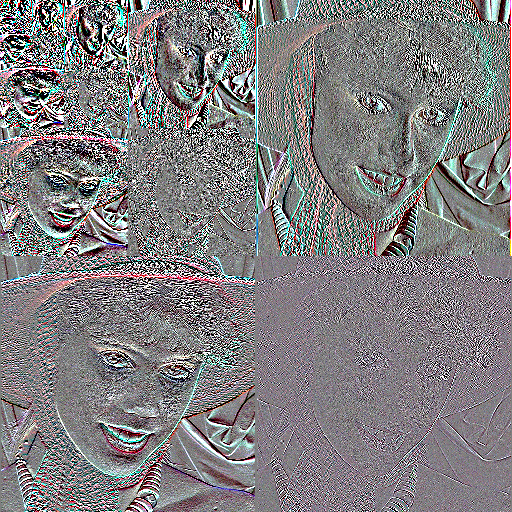
\includegraphics[width=0.3\textwidth]{methods/DWTdiagrams/encodedVisualization.png}
  \caption{Visualization of a 2D Haar transform showing the decomposition of an image}
  \label{fig:encoded_visualization}
\end{figure}




\subsubsection{Compression Properties}

The Haar wavelet transform is particularly effective for image compression because it naturally concentrates energy in the low-resolution approximation coefficients. The detail coefficients (wavelets) typically have smaller magnitudes and can be more aggressively quantized or discarded in lossy compression scenarios. This energy compaction property, combined with the transform's computational efficiency makes the Haar wavelet an attractive choice for practical image compression systems.



The Discrete Wavelet Transform (DWT) is a powerful transform coding technique that decomposes signals into a hierarchy of resolution levels, making it particularly well-suited for image compression. In this work we focus on the Haar wavelet, which is the simplest in the family of wavelets used for this transform. For now on we consider an image as a 1D signal, we later discuss how to convert it to 2D.

\subsubsection{One Dimensional Haar Wavelet Transform in Practice}

Consider a 1D signal with $2^k$ values: $$ \{x_1, x_2, \dots, x_{2^k}\}$$ A naive approach to compression might be to store only the average of adjacent values, resulting in the compressed signal $$A_{k-1} = \{(x_1 + x_2) / 2, (x_3 + x_4) / 2, \dots, (x_{2^k-1} + x_{2^k})/2\}$$ Note that this approach clearly loses information. To enable perfect reconstruction of the original signal, we must also preserve the difference between adjacent values: $$D_{k-1} = \{x_1 - (x_1 + x_2) / 2, x_3 - (x_3 + x_4) / 2, \dots\}$$
Note that the difference of $x_i$ the the mean is completely symmetric to the difference of $x_{i+1}$ to the mean, so we only need to store one detail coefficient. This simple idea is the core of the Haar wavelet transform.

We can apply this operation once and we get a set of $2^k/2$ average coefficients and $2^k/2$ detail coefficients. We can keep applying the operation recursively to the average coefficients until we reach only one pixel of average coefficient. Table~\ref{tab:haar_decomposition} illustrates this process for an 8-pixel signal.

Figure~\ref{fig:haar_decomposition} visualizes this decomposition process, showing the signal (blue) and wavelets (red) at each resolution level. The blue curves represent the averaged signals at decreasing resolutions, while the red curves capture the detail coefficients (differences) that must be preserved for perfect reconstruction.

\begin{table}[h]
  \centering
  \caption{Haar decomposition example for an 8-pixel signal}
  \label{tab:haar_decomposition}
  \begin{tabular}{c c c}
    \toprule
    \textbf{Resolution} & \textbf{Averages} & \textbf{Details} \\
    \midrule
    8 & $[5, \; 8, \; 9, \; 7, \; 4, \; 2, \; 1, \; 3]$ & --- \\
    4 & $[6.5, \; 8, \; 3, \; 2]$ & $[-1.5, \; 1, \; 1, \; -1]$ \\
    2 & $[7.25, \; 2.5]$ & $[-0.75, \; 0.5]$ \\
    1 & $[4.875]$ & $[2.375]$ \\
    \bottomrule
  \end{tabular}
\end{table}

\begin{figure}[ht]
  \centering
  % Haar wavelet decomposition diagram showing signal and wavelets at each resolution level
% Arranged in a 2x2 grid to fit in a single column
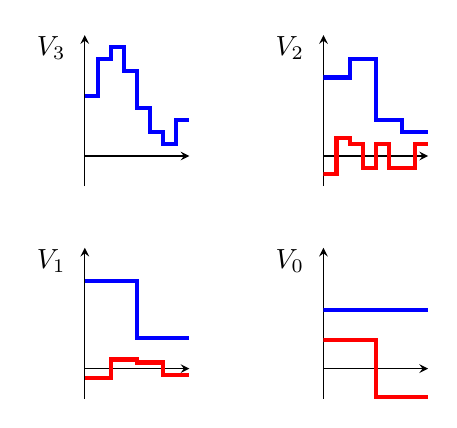
\begin{tikzpicture}
  % Top row: Resolution 8 (V_3) - top left
  \begin{axis}[
    at={(0.13\textwidth,4.5cm)},
    width=0.24\textwidth,
    height=3.5cm,
    xmin=0, xmax=1,
    ymin=-2.5, ymax=10,
    ytick=\empty,
    xtick=\empty,
    axis x line=middle,
    axis y line=center,
  ]
    \addplot[const plot, line width=1.5pt, color=blue] coordinates {
      (0,5) (0.125,5) (0.125,8) (0.25,8) (0.25,9) (0.375,9) (0.375,7) (0.5,7) (0.5,4) (0.625,4) (0.625,2) (0.75,2) (0.75,1) (0.875,1) (0.875,3) (1,3)
    };
  \end{axis}
  \node[anchor=east] at (0.12\textwidth, 6.25cm) {$V_3$};
  
  % Top row: Resolution 4 (V_2) - top right
  \begin{axis}[
    at={(0.38\textwidth,4.5cm)},
    width=0.24\textwidth,
    height=3.5cm,
    xmin=0, xmax=1,
    ymin=-2.5, ymax=10,
    ytick=\empty,
    xtick=\empty,
    axis x line=middle,
    axis y line=center,
  ]
    \addplot[const plot, line width=1.5pt, color=blue] coordinates {
      (0,6.5) (0.25,6.5) (0.25,8) (0.5,8) (0.5,3) (0.75,3) (0.75,2) (1,2)
    };
    \addplot[const plot, line width=1.5pt, color=red] coordinates {
      (0,-1.5) (0.125,-1.5) (0.125,1.5) (0.25,1.5) (0.25,1) (0.375,1) (0.375,-1) (0.5,-1) (0.5,1) (0.625,1) (0.625,-1) (0.75,-1) (0.75,-1) (0.875,-1) (0.875,1) (1,1)
    };
  \end{axis}
  \node[anchor=east] at (0.37\textwidth, 6.25cm) {$V_2$};

  % Bottom row: Resolution 2 (V_1) - bottom left
  \begin{axis}[
    at={(0.13\textwidth,1.8cm)},
    width=0.24\textwidth,
    height=3.5cm,
    xmin=0, xmax=1,
    ymin=-2.5, ymax=10,
    ytick=\empty,
    xtick=\empty,
    axis x line=middle,
    axis y line=center,
  ]
    \addplot[const plot, line width=1.5pt, color=blue] coordinates {
      (0,7.25) (0.5,7.25) (0.5,2.5) (1,2.5)
    };
    \addplot[const plot, line width=1.5pt, color=red] coordinates {
      (0,-0.75) (0.25,-0.75) (0.25,0.75) (0.5,0.75) (0.5,0.5) (0.75,0.5) (0.75,-0.5) (1,-0.5)
    };
  \end{axis}
  \node[anchor=east] at (0.12\textwidth, 3.55cm) {$V_1$};
  
  % Bottom row: Resolution 1 (V_0) - bottom right
  \begin{axis}[
    at={(0.38\textwidth,1.8cm)},
    width=0.24\textwidth,
    height=3.5cm,
    xmin=0, xmax=1,
    ymin=-2.5, ymax=10,
    ytick=\empty,
    xtick=\empty,
    axis x line=middle,
    axis y line=center,
  ]
    \addplot[const plot, line width=1.5pt, color=blue] coordinates {
      (0,4.875) (1,4.875)
    };
    \addplot[const plot, line width=1.5pt, color=red] coordinates {
      (0,2.375) (0.5,2.375) (0.5,-2.375) (1,-2.375)
    };
  \end{axis}
  \node[anchor=east] at (0.37\textwidth, 3.55cm) {$V_0$};

\end{tikzpicture}


  \caption{Haar wavelet decomposition showing signal (blue) and wavelets (red) at each resolution level.}
  \label{fig:haar_decomposition}
\end{figure}

Note that for a given level we can perfectly reconstruct the previous level's average coefficients from the combination of the average coefficient and detail coefficients, so all we need to store in a compression is the set of all detail coefficients and the very last average.

\subsubsection{Theoretical Foundation for Haar Wavelet Transform}

The Haar wavelet transform is founded on a set of nested vector spaces $V^j$ representing piecewise-constant functions at different resolutions, where $V^0 \subset V^1 \subset V^2 \subset \dots$. This nested structure enables a change of basis from the natural basis of scaling functions in $V^{j+1}$ to a basis consisting of the scaling functions from the lower-resolution space $V^j$ together with the wavelet basis functions from the orthogonal complement space $W^j$. The scaling functions provide the coarse approximation, while the wavelets capture the detail information needed for perfect reconstruction. Figure~\ref{fig:basis_functions} visualizes the scaling functions and Haar wavelets for different resolution levels.

\begin{figure*}[hbt]
  \centering
  \begin{minipage}{\textwidth}
    \centering
    % Scaling functions (basis) for V_3: eight piecewise constant functions
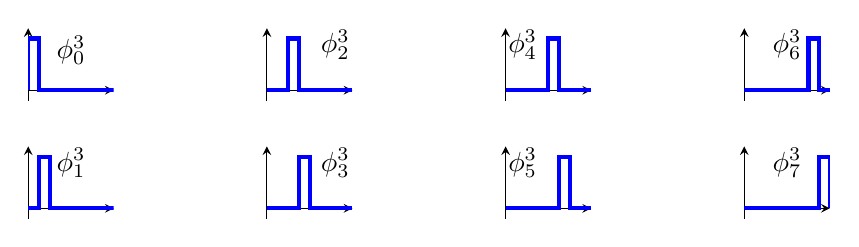
\begin{tikzpicture}
  % Column 1: Scaling functions 1 and 2
  % Scaling function 1: [0, 1/8)
  \begin{axis}[
    at={(0,0)},
    width=0.22\textwidth,
    height=2.5cm,
    xmin=0, xmax=1,
    ymin=-0.2, ymax=1.2,
    ytick=\empty,
    xtick=\empty,
    axis x line=middle,
    axis y line=center,
  ]
    \addplot[const plot, line width=1.5pt, color=blue] coordinates {
      (0,0) (0,1) (0.125,1) (0.125,0) (1,0)
    };
    \node[above] at (0.5, 0.3) {$\phi_0^3$};
  \end{axis}
  % Scaling function 2: [1/8, 1/4)
  \begin{axis}[
    at={(0,-1.5cm)},
    width=0.22\textwidth,
    height=2.5cm,
    xmin=0, xmax=1,
    ymin=-0.2, ymax=1.2,
    ytick=\empty,
    xtick=\empty,
    axis x line=middle,
    axis y line=center,
  ]
    \addplot[const plot, line width=1.5pt, color=blue] coordinates {
      (0,0) (0.125,0) (0.125,1) (0.25,1) (0.25,0) (1,0)
    };
    \node[above] at (0.5, 0.4) {$\phi_1^3$};
  \end{axis}
  
  % Column 2: Scaling functions 3 and 4
  % Scaling function 3: [1/4, 3/8)
  \begin{axis}[
    at={(0.25\textwidth,0)},
    width=0.22\textwidth,
    height=2.5cm,
    xmin=0, xmax=1,
    ymin=-0.2, ymax=1.2,
    ytick=\empty,
    xtick=\empty,
    axis x line=middle,
    axis y line=center,
  ]
    \addplot[const plot, line width=1.5pt, color=blue] coordinates {
      (0,0) (0.25,0) (0.25,1) (0.375,1) (0.375,0) (1,0)
    };
    \node[above] at (0.8, 0.4) {$\phi_2^3$};
  \end{axis}
  % Scaling function 4: [3/8, 1/2)
  \begin{axis}[
    at={(0.25\textwidth,-1.5cm)},
    width=0.22\textwidth,
    height=2.5cm,
    xmin=0, xmax=1,
    ymin=-0.2, ymax=1.2,
    ytick=\empty,
    xtick=\empty,
    axis x line=middle,
    axis y line=center,
  ]
    \addplot[const plot, line width=1.5pt, color=blue] coordinates {
      (0,0) (0.375,0) (0.375,1) (0.5,1) (0.5,0) (1,0)
    };
    \node[above] at (0.8, 0.4) {$\phi_3^3$};
  \end{axis}
  
  % Column 3: Scaling functions 5 and 6
  % Scaling function 5: [1/2, 5/8)
  \begin{axis}[
    at={(0.5\textwidth,0)},
    width=0.22\textwidth,
    height=2.5cm,
    xmin=0, xmax=1,
    ymin=-0.2, ymax=1.2,
    ytick=\empty,
    xtick=\empty,
    axis x line=middle,
    axis y line=center,
  ]
    \addplot[const plot, line width=1.5pt, color=blue] coordinates {
      (0,0) (0.5,0) (0.5,1) (0.625,1) (0.625,0) (1,0)
    };
    \node[above] at (0.2, 0.4) {$\phi_4^3$};
  \end{axis}
  % Scaling function 6: [5/8, 3/4)
  \begin{axis}[
    at={(0.5\textwidth,-1.5cm)},
    width=0.22\textwidth,
    height=2.5cm,
    xmin=0, xmax=1,
    ymin=-0.2, ymax=1.2,
    ytick=\empty,
    xtick=\empty,
    axis x line=middle,
    axis y line=center,
  ]
    \addplot[const plot, line width=1.5pt, color=blue] coordinates {
      (0,0) (0.625,0) (0.625,1) (0.75,1) (0.75,0) (1,0)
    };
    \node[above] at (0.2, 0.4) {$\phi_5^3$};
  \end{axis}
  
  % Column 4: Scaling functions 7 and 8
  % Scaling function 7: [3/4, 7/8)
  \begin{axis}[
    at={(0.75\textwidth,0)},
    width=0.22\textwidth,
    height=2.5cm,
    xmin=0, xmax=1,
    ymin=-0.2, ymax=1.2,
    ytick=\empty,
    xtick=\empty,
    axis x line=middle,
    axis y line=center,
  ]
    \addplot[const plot, line width=1.5pt, color=blue] coordinates {
      (0,0) (0.75,0) (0.75,1) (0.875,1) (0.875,0) (1,0)
    };
    \node[above] at (0.5, 0.4) {$\phi_6^3$};
  \end{axis}
  % Scaling function 8: [7/8, 1)
  \begin{axis}[
    at={(0.75\textwidth,-1.5cm)},
    width=0.22\textwidth,
    height=2.5cm,
    xmin=0, xmax=1,
    ymin=-0.2, ymax=1.2,
    ytick=\empty,
    xtick=\empty,
    axis x line=middle,
    axis y line=center,
  ]
    \addplot[const plot, line width=1.5pt, color=blue] coordinates {
      (0,0) (0.875,0) (0.875,1) (1,1) (1,0)
    };
    \node[above] at (0.5, 0.4) {$\phi_7^3$};
  \end{axis}
\end{tikzpicture}


    \subcaption{Scaling functions (basis) for $V^3$: eight piecewise constant functions.}
    \label{fig:scaling_functions}
  \end{minipage}
  \vspace{0.5cm}
  \begin{minipage}{\textwidth}
    \centering
    % Basis for V_2 (blue) and Haar wavelets basis for W_2 (red)
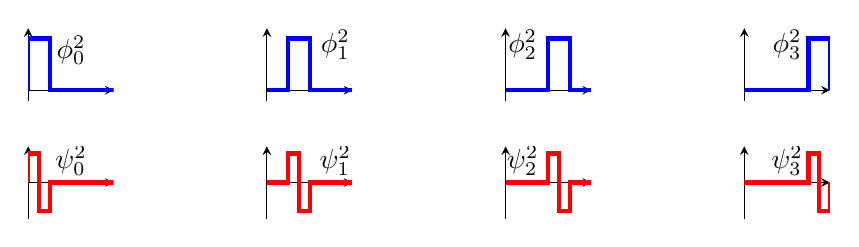
\begin{tikzpicture}
  % V_2 Scaling functions (row above)
  % Scaling function 1: [0, 1/4)
  \begin{axis}[
    at={(0,1.5cm)},
    width=0.22\textwidth,
    height=2.5cm,
    xmin=0, xmax=1,
    ymin=-0.2, ymax=1.2,
    ytick=\empty,
    xtick=\empty,
    axis x line=middle,
    axis y line=center,
  ]
    \addplot[const plot, line width=1.5pt, color=blue] coordinates {
      (0,0) (0,1) (0.25,1) (0.25,0) (1,0)
    };
    \node[above] at (0.5, 0.3) {$\phi_0^2$};
  \end{axis}
  % Scaling function 2: [1/4, 1/2)
  \begin{axis}[
    at={(0.25\textwidth,1.5cm)},
    width=0.22\textwidth,
    height=2.5cm,
    xmin=0, xmax=1,
    ymin=-0.2, ymax=1.2,
    ytick=\empty,
    xtick=\empty,
    axis x line=middle,
    axis y line=center,
  ]
    \addplot[const plot, line width=1.5pt, color=blue] coordinates {
      (0,0) (0.25,0) (0.25,1) (0.5,1) (0.5,0) (1,0)
    };
    \node[above] at (0.8, 0.4) {$\phi_1^2$};
  \end{axis}
  % Scaling function 3: [1/2, 3/4)
  \begin{axis}[
    at={(0.5\textwidth,1.5cm)},
    width=0.22\textwidth,
    height=2.5cm,
    xmin=0, xmax=1,
    ymin=-0.2, ymax=1.2,
    ytick=\empty,
    xtick=\empty,
    axis x line=middle,
    axis y line=center,
  ]
    \addplot[const plot, line width=1.5pt, color=blue] coordinates {
      (0,0) (0.5,0) (0.5,1) (0.75,1) (0.75,0) (1,0)
    };
    \node[above] at (0.2, 0.4) {$\phi_2^2$};
  \end{axis}
  % Scaling function 4: [3/4, 1)
  \begin{axis}[
    at={(0.75\textwidth,1.5cm)},
    width=0.22\textwidth,
    height=2.5cm,
    xmin=0, xmax=1,
    ymin=-0.2, ymax=1.2,
    ytick=\empty,
    xtick=\empty,
    axis x line=middle,
    axis y line=center,
  ]
    \addplot[const plot, line width=1.5pt, color=blue] coordinates {
      (0,0) (0.75,0) (0.75,1) (1,1) (1,0)
    };
    \node[above] at (0.5, 0.4) {$\phi_3^2$};
  \end{axis}
  
  % Wavelet level 2, first: [0, 1/8) vs [1/8, 1/4)
  \begin{axis}[
    at={(0,0)},
    width=0.22\textwidth,
    height=2.5cm,
    xmin=0, xmax=1,
    ymin=-2.5, ymax=2.5,
    ytick=\empty,
    xtick=\empty,
    axis x line=middle,
    axis y line=center,
  ]
    \addplot[const plot, line width=1.5pt, color=red] coordinates {
      (0,0) (0,2) (0.125,2) (0.125,-2) (0.25,-2) (0.25,0) (1,0)
    };
    \node[above] at (0.5, -0.2) {$\psi_0^2$};
  \end{axis}
  % Wavelet level 2, second: [1/4, 3/8) vs [3/8, 1/2)
  \begin{axis}[
    at={(0.25\textwidth,0)},
    width=0.22\textwidth,
    height=2.5cm,
    xmin=0, xmax=1,
    ymin=-2.5, ymax=2.5,
    ytick=\empty,
    xtick=\empty,
    axis x line=middle,
    axis y line=center,
  ]
    \addplot[const plot, line width=1.5pt, color=red] coordinates {
      (0,0) (0.25,0) (0.25,2) (0.375,2) (0.375,-2) (0.5,-2) (0.5,0) (1,0)
    };
    \node[above] at (0.8, -0.2) {$\psi_1^2$};
  \end{axis}
  % Wavelet level 2, third: [1/2, 5/8) vs [5/8, 3/4)
  \begin{axis}[
    at={(0.5\textwidth,0)},
    width=0.22\textwidth,
    height=2.5cm,
    xmin=0, xmax=1,
    ymin=-2.5, ymax=2.5,
    ytick=\empty,
    xtick=\empty,
    axis x line=middle,
    axis y line=center,
  ]
    \addplot[const plot, line width=1.5pt, color=red] coordinates {
      (0,0) (0.5,0) (0.5,2) (0.625,2) (0.625,-2) (0.75,-2) (0.75,0) (1,0)
    };
    \node[above] at (0.2, -0.2) {$\psi_2^2$};
  \end{axis}
  % Wavelet level 2, fourth: [3/4, 7/8) vs [7/8, 1)
  \begin{axis}[
    at={(0.75\textwidth,0)},
    width=0.22\textwidth,
    height=2.5cm,
    xmin=0, xmax=1,
    ymin=-2.5, ymax=2.5,
    ytick=\empty,
    xtick=\empty,
    axis x line=middle,
    axis y line=center,
  ]
    \addplot[const plot, line width=1.5pt, color=red] coordinates {
      (0,0) (0.75,0) (0.75,2) (0.875,2) (0.875,-2) (1,-2) (1,0)
    };
    \node[above] at (0.5, -0.2) {$\psi_3^2$};
  \end{axis}
\end{tikzpicture}


    \subcaption{Basis for $V^2$ (blue) and Haar wavelets basis for $W^2$ (red).}
    \label{fig:wavelet_basis}
  \end{minipage}
  \caption{Haar basis: scaling functions for $V^3$ and scaling functions and wavelets for $V^2$ and $W^2$.}
  \label{fig:basis_functions}
\end{figure*}

A detailed mathematical exposition of the vector space structure, scaling functions, inner products, orthogonality, and the Haar wavelet basis functions is provided in Appendix \ref{apx:haartheory}.




\subsubsection{Two-Dimensional Haar Wavelet Transform}

The 2D Haar wavelet transform generalizes the 1D "averaging and differencing" filter bank to 2D by alternating between operations on rows and columns at each level of the hierarchy.

\paragraph{The Decomposition Algorithm}

The algorithm proceeds recursively as follows:

\begin{enumerate}
\item \textbf{Row Step:} First, perform one step of horizontal pairwise averaging and differencing on the pixel values in each row of the image. This splits the image horizontally into averages (left) and details (right).

\item \textbf{Column Step:} Next, apply vertical pairwise averaging and differencing to each column of the result from the Row Step.
\begin{itemize}
\item This creates four distinct quadrants of coefficients:
\begin{itemize}
\item \textbf{Top-Left:} Averages of averages (coarse approximation).
\item \textbf{Top-Right:} Averages of horizontal details.
\item \textbf{Bottom-Left:} Vertical details of horizontal averages.
\item \textbf{Bottom-Right:} Vertical details of horizontal details (diagonal details).
\end{itemize}
\end{itemize}

\item \textbf{Recursion:} To complete the transformation, repeat this process recursively \textit{only} on the quadrant containing the averages in both directions (the top-left quadrant).
\end{enumerate}

Figure~\ref{fig:encoded_visualization} visualizes this 2D Haar transform decomposition process, showing how an image is decomposed into four quadrants at each level.

\begin{figure}[ht]
  \centering
  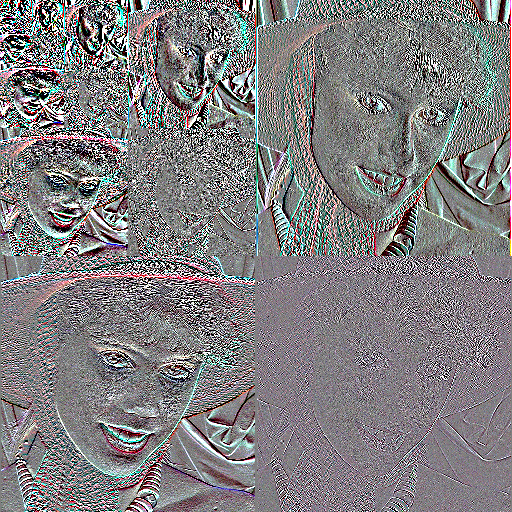
\includegraphics[width=0.3\textwidth]{methods/DWTdiagrams/encodedVisualization.png}
  \caption{Visualization of a 2D Haar transform showing the decomposition of an image}
  \label{fig:encoded_visualization}
\end{figure}




\subsubsection{Compression Properties}

The Haar wavelet transform is particularly effective for image compression because it naturally concentrates energy in the low-resolution approximation coefficients. The detail coefficients (wavelets) typically have smaller magnitudes and can be more aggressively quantized or discarded in lossy compression scenarios. This energy compaction property, combined with the transform's computational efficiency makes the Haar wavelet an attractive choice for practical image compression systems.


\label{methodsec:DWT}

\subsection{Discrete Fourier and Cosine Transforms}
% Content for Fourier Methods subsection
% This file is included in the main conference paper via % Content for Fourier Methods subsection
% This file is included in the main conference paper via % Content for Fourier Methods subsection
% This file is included in the main conference paper via \input{FourierMethods}

Two of the most prevalent transforms in signal processing are the Discrete Fourier Transform (DFT) and its derivative, the Discrete Cosine Transform (DCT). Broadly speaking, these transforms represent the original input as a sum of different wave frequencies. We will first discuss the DFT and its shortcomings, then show how this naturally gives rise to the DCT. 

\subsubsection{The Discrete Fourier Transform in 1 Dimension}

For the DFT, we consider our input as a 1-dimensional signal $x=\{x_0,\dots,x_{N-1}\}$ as described in Section \ref{methodsec:background}\footnote{We shift the indices to start at 0 throughout this section for convenience.}. For Fourier Analysis, it is common to call $x$ a \textbf{time signal}, which is any ordered list of values (in our case, the pixels along the rows and columns of the image). We assume that our signal is periodic modulo $N$, extending to infinity using the relation $x_k=x_{Nm+k}$ for each $m\in\mathbb{Z}$ as shown in Fig. \ref{fig:sigmod}. This way, we can define our basis to be the set of complex waveforms
\begin{equation}
    E=\{E_0,E_1,\dots,E_{N-1}\},\label{eq:dftbasis}
\end{equation}
where
\begin{equation}
    E_k=\{e^{2\pi ik(0)/N}, e^{2\pi ik(1)/N},\dots,e^{2\pi ik(N-1)/N}\}.\label{eq:dftbasiselement}
\end{equation}

\begin{figure}
    \centering
    \includestandalone[width=0.8\linewidth]{methods/Fourierdiagrams/SignalModN}
    \caption{The signal extension of $x\mod N$}
    \label{fig:sigmod}
\end{figure}

As a reminder, complex numbers are of the form $a+bi$, where $a,b\in\mathbb{R}$ and $i=\sqrt{-1}$. Also, we have Euler's identity
\begin{equation}
    e^{i\theta}=\cos\theta+i\sin\theta.
\end{equation}
This means that the basis is effectively made of discrete rotations around the unit circle in the complex plane at different frequencies. An example for the basis $E_1$ for $N=8$ is shown in Fig. \ref{fig:eulerid}. Note that the basis starts at 1 and travels around the unit circle clockwise.

\begin{figure}
    \centering
    \includestandalone[width=0.8\linewidth]{methods/Fourierdiagrams/EulersIdentity}
    \caption{The basis $E_1$ for $N=8$ in the complex plane. Note that these are all the solutions to $\omega^8=1$, the so-called 8th roots of unity.}
    \label{fig:eulerid}
\end{figure}

All of the basis vectors for $N=8$ are represented in Fig. \ref{fig:DFTBasis}, with both the real part (blue) and imaginary part (red). We have chosen $N=8$ for these figures as this will be our choice of block size for the 2D case later in this section. Note that the first basis vector $E_0$ is constant, while each subsequent vector has increasing frequency.

\begin{figure*}
    \centering
    \begin{minipage}{\textwidth}
        \centering
        \includestandalone[width=1\linewidth]{methods/Fourierdiagrams/DFTBasis}
    \end{minipage}
    \caption{Every DFT basis vector for $N=8$. The first row is $E_0,E_1,E_2,E_3$, and the second row is $E_4,E_5,E_6,E)7$. }
    \label{fig:DFTBasis}
\end{figure*}

We can transform the signal into a representation in our new basis using the following formula:
\begin{equation}
    X_k=\frac{1}{\sqrt{N}}\sum_{m=0}^{N-1}x_me^{-2\pi ikm/N}.\label{eq:dfttransform}
\end{equation}
This forms a new signal $X=\{X_0,X_2,\dots,X_{N-1}\}$ (note that the $1/\sqrt{N}$ term is just a normalization). We say that $X$ lives in the \textbf{frequency domain}. With the change of basis, each $X_k$ is now the corresponding coefficient for the basis vector $E_k$. The first coefficient $X_0$ is called the \textbf{DC coefficient}, and corresponds to the average value of the signal since $E_0$ is constant. All other coefficients are called \textbf{AC coefficients}\footnote{The terms DC and AC come from an electrical context, meaning \textit{direct current} and \textit{alternating current}}. This transform is lossless and invertible, with each value in the original time signal retrieved by calculating

\begin{equation}
    X_k=\frac{1}{\sqrt{N}}\sum_{m=0}^{N-1}X_me^{2\pi ikm/N}.\label{eq:idfttransform}
\end{equation}

We call equations \ref{eq:dfttransform} and \ref{eq:idfttransform} the \textbf{forward} and \textbf{inverse} transforms, respectively. These formulas are derived from taking the normal \textbf{inner product} in the vector space $\mathbb{C}^N$. Those interested in the mathematical background should refer to Broughton \cite{broughton2009discrete}. 

\subsubsection{Applying the Discrete Fourier Transform to a 2D Image}

We now discuss how to apply the 1D DFT to an image. As discussed in Section \ref{methodsec:background}, we represent the image as a 2D array of pixels in the YCbCr colorspace described in Section \ref{sec:intro}. We then break the image up into 8x8 blocks of pixels, and apply the 1D DFT along each row and each column of the block. A visualization for the transform is provided in Fig. \ref{fig:dftvis}.

\begin{figure}
    \centering
    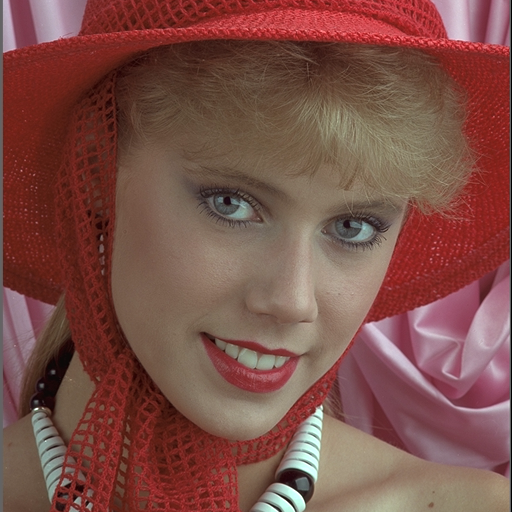
\includegraphics[width=0.4\linewidth]{methods/Fourierdiagrams/OriginalImg.png}\hfill
    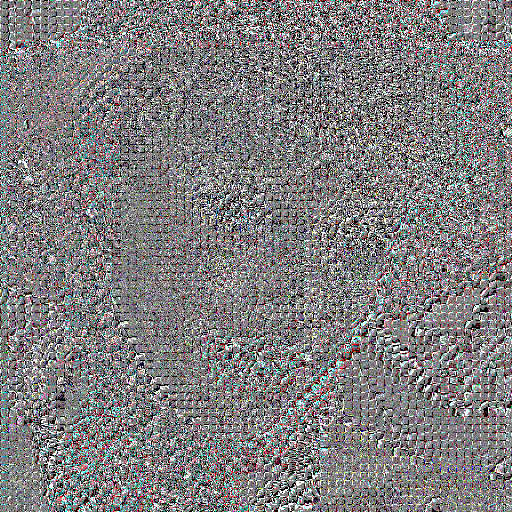
\includegraphics[width=0.4\linewidth]{methods/Fourierdiagrams/DFTVis.png}
    \caption{An original Image from the Kodak dataset (left) and a visualization after applying the DFT (right). The image is $512\times 512$ pixels, and at a closer look one can see block-like shapes where the transform has been applied to 8x8 chunks.}
    \label{fig:dftvis}
\end{figure}

In Section \ref{methodsec:background} we mentioned that the goal of the transform was to reduce entropy as defined in Section \ref{sec:intro}. If the image was random noise, we would generally not expect this to be the case. However, since pixels are correlated with those around them in an image, we don't expect sharp changes in pixel values. This means in our new basis, the coefficients for the lower frequency basis vectors $E_0,E_1,E_2,\dots$ have larger values than the coefficients for the higher frequency basis vectors $\dots,E_{N-2},E_{N-1}$. This results in a lower entropy, which combined with quantization discussed in Section \ref{methodsec:quant} allows for solid compression ratios.

\subsubsection{Problems with the DFT}
At this point, we have built up the DFT as a change of basis on an image to represent it as frequency components where we expect the energy of the signal to be concentrated in lower frequency coefficients. However, there are several problems that arise that greatly limit the ability of the DFT to achieve great compression.
\begin{enumerate}
    \item The DFT is slow. A raw application of Equation \ref{eq:dfttransform} requires $\mathcal{O}(N^2)$ complex multiplications, which means for a 2D Image the runtime is $\mathcal{O}(NM)^2$, for an $N\times M$ image (or just $\mathcal{O}(N^4)$ if we assume that the image is square).
    \item The output to the DFT is complex-valued. Since we are using complex waveforms as a basis, we are thinking of our pixels as living in the complex plane $\mathbb{C}$, not the real numbers $\mathbb{R}$. Complex values take twice as much space to store as real numbers.
    \item The DFT does not fully eliminate large values in high frequency coefficients. Since the DFT assumes the signal $x$ is periodic modulo $N$, if $|x_0-x_{N-1}|$ is large, then there will be a high frequency jump in the signal resulting in larger terms (Refer back to Fig. \ref{fig:sigmod} for an example). 
\end{enumerate}
The first issue of runtime can be addressed by using a clever algorithm called the Fast Fourier Transform (FFT), which exploits the symmetries of complex waveforms to reduce the runtime to $\mathcal{O}(N^2\log N)$ for an $N\times N$ pixel image. More details are provided in Appendix \ref{apx:fft}. At first glance, the following issues are not so easy to fix. However, by changing the assumptions about our signal $x$ slightly, we are able to solve both problems simultaneously. This is exactly what the Discrete Cosine Transform (DCT) does.

\subsubsection{The Discrete Cosine Transform}
The idea behind the DCT is very simple. Starting with our signal $x=\{x_0,\dots,x_{N-1}\}$, we first \textbf{mirror} our signal to one of length $2N$, giving a new signal
\begin{equation}
    \hat{x}=\{x_0,\dots,x_{N-1},x_{N-1},\dots,x_0\},
    \label{eq:dctsig}
\end{equation}
which we then assume is periodic modulo $2N$ instead as shown in Fig. \ref{fig:dctextension} in the $N=8$ case. We then perform the DFT on this extended signal to get a transformed signal $\hat{X}=\{X_0,\dots,X_{2N-1}\}$. With a little bit of unpacking, one can start with Equation \ref{eq:dfttransform} and show that the coefficients for the resulting transform are given by
\begin{align}
    X_k&=\sum_{m=0}^{2N-1}x_me^{-2\pi ikm/2N}\label{eq:2ndft}\\
    &=2e^{2\pi ik/2N}\sum_{m=0}^{N-1}x_m\cos\bigg(\frac{\pi k(m+\tfrac{1}{2})}{2N}\bigg),\label{eq:predcttransform}
\end{align}
where we have taken advantage of the symmetry in our mirrored signal $\hat{x}$. These terms are almost real, and after applying a phase shift and normalizing we get the final DCT coefficients given by
\begin{equation}
    X_k=\sqrt{\frac{c_k}{N}}\sum_{m=0}^{N-1}x_m\cos\bigg(\frac{\pi k(m+\tfrac{1}{2})}{N}\bigg),\label{eq:dcttransform}
\end{equation}
taking $c_k=1$ if $k=0$ and $c_k=2$ otherwise. Note that this gives us only half of the $2N$ coefficients that we expect. This is sufficient because due to the symmetry of the signal, the remaining coefficients are recovered by the identity
\begin{equation}
    X_{2N-r}=-X_r\quad\text{for }r=0,1,\dots,N.\label{eq:dctrelation}
\end{equation}
Notice that this forces $X_N=0$. The math behind these relations can be found in Broughton \cite{broughton2009discrete}. We now notice the 2 critical facts about the result.
\begin{enumerate}
    \item The DCT is real-valued. The mirrored nature of the extended signal $\hat{x}$ has washed out all imaginary components.
    \item The new signal also has no potential for sharp gaps when moving to a new period, meaning smaller values in the higher frequency coefficients.
\end{enumerate}
These are exactly the two problems that we wanted to improve on for the DFT, and we see that the DCT achieves both by mirroring the signal and using the relation in Equation \ref{eq:dctrelation} to not increase space. To apply the DCT to an image, one can simply follow the same steps for the DFT, except to mirror each row and each column of pixels in each chunk before applying the transform, and saving the first half of the result. See Section \ref{sec:results} for just how much more effective the DCT is over the DFT.

\begin{figure}
    \centering
    \includestandalone[width=0.8\linewidth]{methods/Fourierdiagrams/DCTExtension}
    \caption{The new signal $\hat{x}$ extended modulo $2N$ for $N=8$. Note that there are no sharp gaps at the extension point.}
    \label{fig:dctextension}
\end{figure}

Two of the most prevalent transforms in signal processing are the Discrete Fourier Transform (DFT) and its derivative, the Discrete Cosine Transform (DCT). Broadly speaking, these transforms represent the original input as a sum of different wave frequencies. We will first discuss the DFT and its shortcomings, then show how this naturally gives rise to the DCT. 

\subsubsection{The Discrete Fourier Transform in 1 Dimension}

For the DFT, we consider our input as a 1-dimensional signal $x=\{x_0,\dots,x_{N-1}\}$ as described in Section \ref{methodsec:background}\footnote{We shift the indices to start at 0 throughout this section for convenience.}. For Fourier Analysis, it is common to call $x$ a \textbf{time signal}, which is any ordered list of values (in our case, the pixels along the rows and columns of the image). We assume that our signal is periodic modulo $N$, extending to infinity using the relation $x_k=x_{Nm+k}$ for each $m\in\mathbb{Z}$ as shown in Fig. \ref{fig:sigmod}. This way, we can define our basis to be the set of complex waveforms
\begin{equation}
    E=\{E_0,E_1,\dots,E_{N-1}\},\label{eq:dftbasis}
\end{equation}
where
\begin{equation}
    E_k=\{e^{2\pi ik(0)/N}, e^{2\pi ik(1)/N},\dots,e^{2\pi ik(N-1)/N}\}.\label{eq:dftbasiselement}
\end{equation}

\begin{figure}
    \centering
    \includestandalone[width=0.8\linewidth]{methods/Fourierdiagrams/SignalModN}
    \caption{The signal extension of $x\mod N$}
    \label{fig:sigmod}
\end{figure}

As a reminder, complex numbers are of the form $a+bi$, where $a,b\in\mathbb{R}$ and $i=\sqrt{-1}$. Also, we have Euler's identity
\begin{equation}
    e^{i\theta}=\cos\theta+i\sin\theta.
\end{equation}
This means that the basis is effectively made of discrete rotations around the unit circle in the complex plane at different frequencies. An example for the basis $E_1$ for $N=8$ is shown in Fig. \ref{fig:eulerid}. Note that the basis starts at 1 and travels around the unit circle clockwise.

\begin{figure}
    \centering
    \includestandalone[width=0.8\linewidth]{methods/Fourierdiagrams/EulersIdentity}
    \caption{The basis $E_1$ for $N=8$ in the complex plane. Note that these are all the solutions to $\omega^8=1$, the so-called 8th roots of unity.}
    \label{fig:eulerid}
\end{figure}

All of the basis vectors for $N=8$ are represented in Fig. \ref{fig:DFTBasis}, with both the real part (blue) and imaginary part (red). We have chosen $N=8$ for these figures as this will be our choice of block size for the 2D case later in this section. Note that the first basis vector $E_0$ is constant, while each subsequent vector has increasing frequency.

\begin{figure*}
    \centering
    \begin{minipage}{\textwidth}
        \centering
        \includestandalone[width=1\linewidth]{methods/Fourierdiagrams/DFTBasis}
    \end{minipage}
    \caption{Every DFT basis vector for $N=8$. The first row is $E_0,E_1,E_2,E_3$, and the second row is $E_4,E_5,E_6,E)7$. }
    \label{fig:DFTBasis}
\end{figure*}

We can transform the signal into a representation in our new basis using the following formula:
\begin{equation}
    X_k=\frac{1}{\sqrt{N}}\sum_{m=0}^{N-1}x_me^{-2\pi ikm/N}.\label{eq:dfttransform}
\end{equation}
This forms a new signal $X=\{X_0,X_2,\dots,X_{N-1}\}$ (note that the $1/\sqrt{N}$ term is just a normalization). We say that $X$ lives in the \textbf{frequency domain}. With the change of basis, each $X_k$ is now the corresponding coefficient for the basis vector $E_k$. The first coefficient $X_0$ is called the \textbf{DC coefficient}, and corresponds to the average value of the signal since $E_0$ is constant. All other coefficients are called \textbf{AC coefficients}\footnote{The terms DC and AC come from an electrical context, meaning \textit{direct current} and \textit{alternating current}}. This transform is lossless and invertible, with each value in the original time signal retrieved by calculating

\begin{equation}
    X_k=\frac{1}{\sqrt{N}}\sum_{m=0}^{N-1}X_me^{2\pi ikm/N}.\label{eq:idfttransform}
\end{equation}

We call equations \ref{eq:dfttransform} and \ref{eq:idfttransform} the \textbf{forward} and \textbf{inverse} transforms, respectively. These formulas are derived from taking the normal \textbf{inner product} in the vector space $\mathbb{C}^N$. Those interested in the mathematical background should refer to Broughton \cite{broughton2009discrete}. 

\subsubsection{Applying the Discrete Fourier Transform to a 2D Image}

We now discuss how to apply the 1D DFT to an image. As discussed in Section \ref{methodsec:background}, we represent the image as a 2D array of pixels in the YCbCr colorspace described in Section \ref{sec:intro}. We then break the image up into 8x8 blocks of pixels, and apply the 1D DFT along each row and each column of the block. A visualization for the transform is provided in Fig. \ref{fig:dftvis}.

\begin{figure}
    \centering
    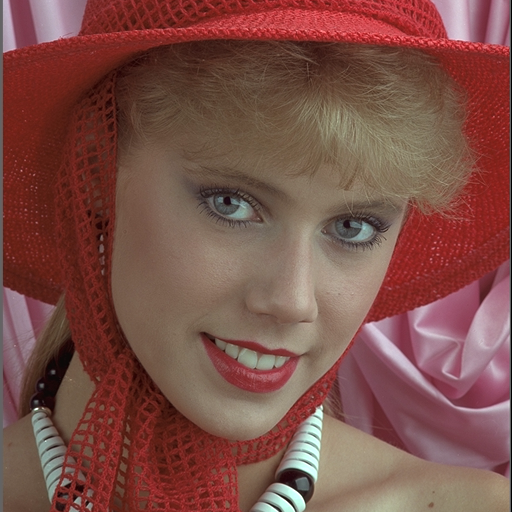
\includegraphics[width=0.4\linewidth]{methods/Fourierdiagrams/OriginalImg.png}\hfill
    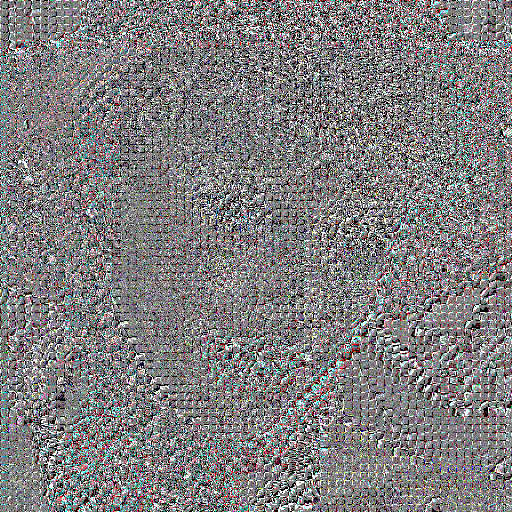
\includegraphics[width=0.4\linewidth]{methods/Fourierdiagrams/DFTVis.png}
    \caption{An original Image from the Kodak dataset (left) and a visualization after applying the DFT (right). The image is $512\times 512$ pixels, and at a closer look one can see block-like shapes where the transform has been applied to 8x8 chunks.}
    \label{fig:dftvis}
\end{figure}

In Section \ref{methodsec:background} we mentioned that the goal of the transform was to reduce entropy as defined in Section \ref{sec:intro}. If the image was random noise, we would generally not expect this to be the case. However, since pixels are correlated with those around them in an image, we don't expect sharp changes in pixel values. This means in our new basis, the coefficients for the lower frequency basis vectors $E_0,E_1,E_2,\dots$ have larger values than the coefficients for the higher frequency basis vectors $\dots,E_{N-2},E_{N-1}$. This results in a lower entropy, which combined with quantization discussed in Section \ref{methodsec:quant} allows for solid compression ratios.

\subsubsection{Problems with the DFT}
At this point, we have built up the DFT as a change of basis on an image to represent it as frequency components where we expect the energy of the signal to be concentrated in lower frequency coefficients. However, there are several problems that arise that greatly limit the ability of the DFT to achieve great compression.
\begin{enumerate}
    \item The DFT is slow. A raw application of Equation \ref{eq:dfttransform} requires $\mathcal{O}(N^2)$ complex multiplications, which means for a 2D Image the runtime is $\mathcal{O}(NM)^2$, for an $N\times M$ image (or just $\mathcal{O}(N^4)$ if we assume that the image is square).
    \item The output to the DFT is complex-valued. Since we are using complex waveforms as a basis, we are thinking of our pixels as living in the complex plane $\mathbb{C}$, not the real numbers $\mathbb{R}$. Complex values take twice as much space to store as real numbers.
    \item The DFT does not fully eliminate large values in high frequency coefficients. Since the DFT assumes the signal $x$ is periodic modulo $N$, if $|x_0-x_{N-1}|$ is large, then there will be a high frequency jump in the signal resulting in larger terms (Refer back to Fig. \ref{fig:sigmod} for an example). 
\end{enumerate}
The first issue of runtime can be addressed by using a clever algorithm called the Fast Fourier Transform (FFT), which exploits the symmetries of complex waveforms to reduce the runtime to $\mathcal{O}(N^2\log N)$ for an $N\times N$ pixel image. More details are provided in Appendix \ref{apx:fft}. At first glance, the following issues are not so easy to fix. However, by changing the assumptions about our signal $x$ slightly, we are able to solve both problems simultaneously. This is exactly what the Discrete Cosine Transform (DCT) does.

\subsubsection{The Discrete Cosine Transform}
The idea behind the DCT is very simple. Starting with our signal $x=\{x_0,\dots,x_{N-1}\}$, we first \textbf{mirror} our signal to one of length $2N$, giving a new signal
\begin{equation}
    \hat{x}=\{x_0,\dots,x_{N-1},x_{N-1},\dots,x_0\},
    \label{eq:dctsig}
\end{equation}
which we then assume is periodic modulo $2N$ instead as shown in Fig. \ref{fig:dctextension} in the $N=8$ case. We then perform the DFT on this extended signal to get a transformed signal $\hat{X}=\{X_0,\dots,X_{2N-1}\}$. With a little bit of unpacking, one can start with Equation \ref{eq:dfttransform} and show that the coefficients for the resulting transform are given by
\begin{align}
    X_k&=\sum_{m=0}^{2N-1}x_me^{-2\pi ikm/2N}\label{eq:2ndft}\\
    &=2e^{2\pi ik/2N}\sum_{m=0}^{N-1}x_m\cos\bigg(\frac{\pi k(m+\tfrac{1}{2})}{2N}\bigg),\label{eq:predcttransform}
\end{align}
where we have taken advantage of the symmetry in our mirrored signal $\hat{x}$. These terms are almost real, and after applying a phase shift and normalizing we get the final DCT coefficients given by
\begin{equation}
    X_k=\sqrt{\frac{c_k}{N}}\sum_{m=0}^{N-1}x_m\cos\bigg(\frac{\pi k(m+\tfrac{1}{2})}{N}\bigg),\label{eq:dcttransform}
\end{equation}
taking $c_k=1$ if $k=0$ and $c_k=2$ otherwise. Note that this gives us only half of the $2N$ coefficients that we expect. This is sufficient because due to the symmetry of the signal, the remaining coefficients are recovered by the identity
\begin{equation}
    X_{2N-r}=-X_r\quad\text{for }r=0,1,\dots,N.\label{eq:dctrelation}
\end{equation}
Notice that this forces $X_N=0$. The math behind these relations can be found in Broughton \cite{broughton2009discrete}. We now notice the 2 critical facts about the result.
\begin{enumerate}
    \item The DCT is real-valued. The mirrored nature of the extended signal $\hat{x}$ has washed out all imaginary components.
    \item The new signal also has no potential for sharp gaps when moving to a new period, meaning smaller values in the higher frequency coefficients.
\end{enumerate}
These are exactly the two problems that we wanted to improve on for the DFT, and we see that the DCT achieves both by mirroring the signal and using the relation in Equation \ref{eq:dctrelation} to not increase space. To apply the DCT to an image, one can simply follow the same steps for the DFT, except to mirror each row and each column of pixels in each chunk before applying the transform, and saving the first half of the result. See Section \ref{sec:results} for just how much more effective the DCT is over the DFT.

\begin{figure}
    \centering
    \includestandalone[width=0.8\linewidth]{methods/Fourierdiagrams/DCTExtension}
    \caption{The new signal $\hat{x}$ extended modulo $2N$ for $N=8$. Note that there are no sharp gaps at the extension point.}
    \label{fig:dctextension}
\end{figure}

Two of the most prevalent transforms in signal processing are the Discrete Fourier Transform (DFT) and its derivative, the Discrete Cosine Transform (DCT). Broadly speaking, these transforms represent the original input as a sum of different wave frequencies. We will first discuss the DFT and its shortcomings, then show how this naturally gives rise to the DCT. 

\subsubsection{The Discrete Fourier Transform in 1 Dimension}

For the DFT, we consider our input as a 1-dimensional signal $x=\{x_0,\dots,x_{N-1}\}$ as described in Section \ref{methodsec:background}\footnote{We shift the indices to start at 0 throughout this section for convenience.}. For Fourier Analysis, it is common to call $x$ a \textbf{time signal}, which is any ordered list of values (in our case, the pixels along the rows and columns of the image). We assume that our signal is periodic modulo $N$, extending to infinity using the relation $x_k=x_{Nm+k}$ for each $m\in\mathbb{Z}$ as shown in Fig. \ref{fig:sigmod}. This way, we can define our basis to be the set of complex waveforms
\begin{equation}
    E=\{E_0,E_1,\dots,E_{N-1}\},\label{eq:dftbasis}
\end{equation}
where
\begin{equation}
    E_k=\{e^{2\pi ik(0)/N}, e^{2\pi ik(1)/N},\dots,e^{2\pi ik(N-1)/N}\}.\label{eq:dftbasiselement}
\end{equation}

\begin{figure}
    \centering
    \includestandalone[width=0.8\linewidth]{methods/Fourierdiagrams/SignalModN}
    \caption{The signal extension of $x\mod N$}
    \label{fig:sigmod}
\end{figure}

As a reminder, complex numbers are of the form $a+bi$, where $a,b\in\mathbb{R}$ and $i=\sqrt{-1}$. Also, we have Euler's identity
\begin{equation}
    e^{i\theta}=\cos\theta+i\sin\theta.
\end{equation}
This means that the basis is effectively made of discrete rotations around the unit circle in the complex plane at different frequencies. An example for the basis $E_1$ for $N=8$ is shown in Fig. \ref{fig:eulerid}. Note that the basis starts at 1 and travels around the unit circle clockwise.

\begin{figure}
    \centering
    \includestandalone[width=0.8\linewidth]{methods/Fourierdiagrams/EulersIdentity}
    \caption{The basis $E_1$ for $N=8$ in the complex plane. Note that these are all the solutions to $\omega^8=1$, the so-called 8th roots of unity.}
    \label{fig:eulerid}
\end{figure}

All of the basis vectors for $N=8$ are represented in Fig. \ref{fig:DFTBasis}, with both the real part (blue) and imaginary part (red). We have chosen $N=8$ for these figures as this will be our choice of block size for the 2D case later in this section. Note that the first basis vector $E_0$ is constant, while each subsequent vector has increasing frequency.

\begin{figure*}
    \centering
    \begin{minipage}{\textwidth}
        \centering
        \includestandalone[width=1\linewidth]{methods/Fourierdiagrams/DFTBasis}
    \end{minipage}
    \caption{Every DFT basis vector for $N=8$. The first row is $E_0,E_1,E_2,E_3$, and the second row is $E_4,E_5,E_6,E)7$. }
    \label{fig:DFTBasis}
\end{figure*}

We can transform the signal into a representation in our new basis using the following formula:
\begin{equation}
    X_k=\frac{1}{\sqrt{N}}\sum_{m=0}^{N-1}x_me^{-2\pi ikm/N}.\label{eq:dfttransform}
\end{equation}
This forms a new signal $X=\{X_0,X_2,\dots,X_{N-1}\}$ (note that the $1/\sqrt{N}$ term is just a normalization). We say that $X$ lives in the \textbf{frequency domain}. With the change of basis, each $X_k$ is now the corresponding coefficient for the basis vector $E_k$. The first coefficient $X_0$ is called the \textbf{DC coefficient}, and corresponds to the average value of the signal since $E_0$ is constant. All other coefficients are called \textbf{AC coefficients}\footnote{The terms DC and AC come from an electrical context, meaning \textit{direct current} and \textit{alternating current}}. This transform is lossless and invertible, with each value in the original time signal retrieved by calculating

\begin{equation}
    X_k=\frac{1}{\sqrt{N}}\sum_{m=0}^{N-1}X_me^{2\pi ikm/N}.\label{eq:idfttransform}
\end{equation}

We call equations \ref{eq:dfttransform} and \ref{eq:idfttransform} the \textbf{forward} and \textbf{inverse} transforms, respectively. These formulas are derived from taking the normal \textbf{inner product} in the vector space $\mathbb{C}^N$. Those interested in the mathematical background should refer to Broughton \cite{broughton2009discrete}. 

\subsubsection{Applying the Discrete Fourier Transform to a 2D Image}

We now discuss how to apply the 1D DFT to an image. As discussed in Section \ref{methodsec:background}, we represent the image as a 2D array of pixels in the YCbCr colorspace described in Section \ref{sec:intro}. We then break the image up into 8x8 blocks of pixels, and apply the 1D DFT along each row and each column of the block. A visualization for the transform is provided in Fig. \ref{fig:dftvis}.

\begin{figure}
    \centering
    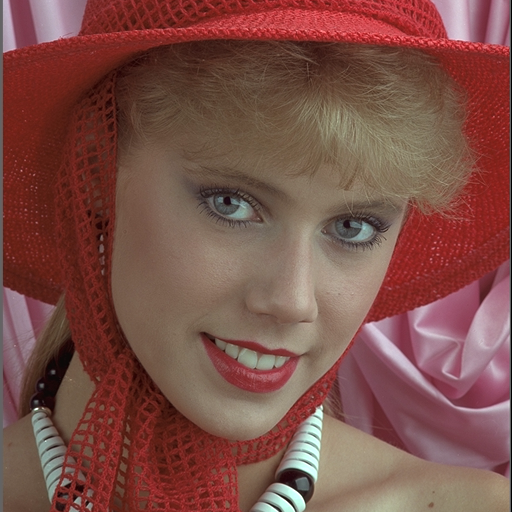
\includegraphics[width=0.4\linewidth]{methods/Fourierdiagrams/OriginalImg.png}\hfill
    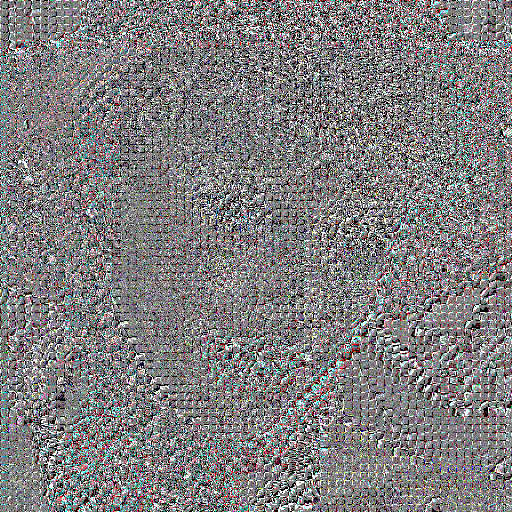
\includegraphics[width=0.4\linewidth]{methods/Fourierdiagrams/DFTVis.png}
    \caption{An original Image from the Kodak dataset (left) and a visualization after applying the DFT (right). The image is $512\times 512$ pixels, and at a closer look one can see block-like shapes where the transform has been applied to 8x8 chunks.}
    \label{fig:dftvis}
\end{figure}

In Section \ref{methodsec:background} we mentioned that the goal of the transform was to reduce entropy as defined in Section \ref{sec:intro}. If the image was random noise, we would generally not expect this to be the case. However, since pixels are correlated with those around them in an image, we don't expect sharp changes in pixel values. This means in our new basis, the coefficients for the lower frequency basis vectors $E_0,E_1,E_2,\dots$ have larger values than the coefficients for the higher frequency basis vectors $\dots,E_{N-2},E_{N-1}$. This results in a lower entropy, which combined with quantization discussed in Section \ref{methodsec:quant} allows for solid compression ratios.

\subsubsection{Problems with the DFT}
At this point, we have built up the DFT as a change of basis on an image to represent it as frequency components where we expect the energy of the signal to be concentrated in lower frequency coefficients. However, there are several problems that arise that greatly limit the ability of the DFT to achieve great compression.
\begin{enumerate}
    \item The DFT is slow. A raw application of Equation \ref{eq:dfttransform} requires $\mathcal{O}(N^2)$ complex multiplications, which means for a 2D Image the runtime is $\mathcal{O}(NM)^2$, for an $N\times M$ image (or just $\mathcal{O}(N^4)$ if we assume that the image is square).
    \item The output to the DFT is complex-valued. Since we are using complex waveforms as a basis, we are thinking of our pixels as living in the complex plane $\mathbb{C}$, not the real numbers $\mathbb{R}$. Complex values take twice as much space to store as real numbers.
    \item The DFT does not fully eliminate large values in high frequency coefficients. Since the DFT assumes the signal $x$ is periodic modulo $N$, if $|x_0-x_{N-1}|$ is large, then there will be a high frequency jump in the signal resulting in larger terms (Refer back to Fig. \ref{fig:sigmod} for an example). 
\end{enumerate}
The first issue of runtime can be addressed by using a clever algorithm called the Fast Fourier Transform (FFT), which exploits the symmetries of complex waveforms to reduce the runtime to $\mathcal{O}(N^2\log N)$ for an $N\times N$ pixel image. More details are provided in Appendix \ref{apx:fft}. At first glance, the following issues are not so easy to fix. However, by changing the assumptions about our signal $x$ slightly, we are able to solve both problems simultaneously. This is exactly what the Discrete Cosine Transform (DCT) does.

\subsubsection{The Discrete Cosine Transform}
The idea behind the DCT is very simple. Starting with our signal $x=\{x_0,\dots,x_{N-1}\}$, we first \textbf{mirror} our signal to one of length $2N$, giving a new signal
\begin{equation}
    \hat{x}=\{x_0,\dots,x_{N-1},x_{N-1},\dots,x_0\},
    \label{eq:dctsig}
\end{equation}
which we then assume is periodic modulo $2N$ instead as shown in Fig. \ref{fig:dctextension} in the $N=8$ case. We then perform the DFT on this extended signal to get a transformed signal $\hat{X}=\{X_0,\dots,X_{2N-1}\}$. With a little bit of unpacking, one can start with Equation \ref{eq:dfttransform} and show that the coefficients for the resulting transform are given by
\begin{align}
    X_k&=\sum_{m=0}^{2N-1}x_me^{-2\pi ikm/2N}\label{eq:2ndft}\\
    &=2e^{2\pi ik/2N}\sum_{m=0}^{N-1}x_m\cos\bigg(\frac{\pi k(m+\tfrac{1}{2})}{2N}\bigg),\label{eq:predcttransform}
\end{align}
where we have taken advantage of the symmetry in our mirrored signal $\hat{x}$. These terms are almost real, and after applying a phase shift and normalizing we get the final DCT coefficients given by
\begin{equation}
    X_k=\sqrt{\frac{c_k}{N}}\sum_{m=0}^{N-1}x_m\cos\bigg(\frac{\pi k(m+\tfrac{1}{2})}{N}\bigg),\label{eq:dcttransform}
\end{equation}
taking $c_k=1$ if $k=0$ and $c_k=2$ otherwise. Note that this gives us only half of the $2N$ coefficients that we expect. This is sufficient because due to the symmetry of the signal, the remaining coefficients are recovered by the identity
\begin{equation}
    X_{2N-r}=-X_r\quad\text{for }r=0,1,\dots,N.\label{eq:dctrelation}
\end{equation}
Notice that this forces $X_N=0$. The math behind these relations can be found in Broughton \cite{broughton2009discrete}. We now notice the 2 critical facts about the result.
\begin{enumerate}
    \item The DCT is real-valued. The mirrored nature of the extended signal $\hat{x}$ has washed out all imaginary components.
    \item The new signal also has no potential for sharp gaps when moving to a new period, meaning smaller values in the higher frequency coefficients.
\end{enumerate}
These are exactly the two problems that we wanted to improve on for the DFT, and we see that the DCT achieves both by mirroring the signal and using the relation in Equation \ref{eq:dctrelation} to not increase space. To apply the DCT to an image, one can simply follow the same steps for the DFT, except to mirror each row and each column of pixels in each chunk before applying the transform, and saving the first half of the result. See Section \ref{sec:results} for just how much more effective the DCT is over the DFT.

\begin{figure}
    \centering
    \includestandalone[width=0.8\linewidth]{methods/Fourierdiagrams/DCTExtension}
    \caption{The new signal $\hat{x}$ extended modulo $2N$ for $N=8$. Note that there are no sharp gaps at the extension point.}
    \label{fig:dctextension}
\end{figure}
\label{methodsec:fourier}


\subsection{The S+P Transform}

\subsubsection{Motivation and High-Level Overview}

To address the need for invertibility without inflating the dynamic range in the process of compression, the S+P transform (Sequential transform + Prediction), originally proposed by Said and Pearlman~\cite{said1993sp}, employs a simple combination of a Haar-like multiresolution transform (the ``S'' stage) and an embedded predictive coding stage (the ``P'' stage).

In the broader context of our project, we treat S+P as a hybrid transform that lives between classical wavelet/subband decompositions(transform) and purely predictive schemes. Earlier sections introduce transform coding and the Haar wavelet; here, we focus on what S+P adds on top of that baseline, and how those additions behave inside our JPEG-style pipeline.

Operationally, S+P still proceeds along one-dimensional signals (rows or columns of an image). The S stage performs an integer lifting-style average/difference, producing lowpass (approximate local averages) and highpass (local differences). The P stage then applies an \emph{integer} prediction filter directly to the highpass branch, aiming to decorrelate it further before quantization and entropy coding. Recursively applying S+P to the lowpass component yields the same LL/HL/LH/HH multiresolution layout as Haar, but with much stronger whitening in the highpass bands and stricter control over rounding and borders.

\subsubsection{Sequential Transform (S) Recap}

We briefly recall the 1D S stage, which is the integer analogue of the Haar lifting step. Let $c[n]$ be a sequence of integer samples of length $N$. For each pair $(c[2n], c[2n+1])$ we define
\begin{align}
    d_1[n] &= c[2n+1] - c[2n], \\
    s[n]   &= c[2n] + \left\lfloor \frac{d_1[n]}{2} \right\rfloor,
\end{align}
for $n = 0, \dots, \lfloor N/2 \rfloor - 1$. Here $s[n]$ acts as a local average, while $d_1[n]$ stores the corresponding difference as detail.

This mapping is exactly reversible with integer arithmetic:
\begin{align}
    c[2n]   &= s[n] - \left\lfloor \frac{d_1[n]}{2} \right\rfloor, \\
    c[2n+1] &= c[2n] + d_1[n].
\end{align}
No fractional bits are introduced: only additions, subtractions, and integer floor-divisions by powers of two are used. Applying this S step to all rows and then all columns, and recursing only on the LL quadrant, gives the same multilevel LL/HL/LH/HH pyramid described for the Haar transform, but now entirely in integers. As shown in Figure ~\ref{fig:sp_level1}, each level of S+P transform decompose the image into the four subbands: LL carries the coarse approximation as the mean image of the original, HL captures vertical edges, LH captures horizontal edges, and HH captures fine diagonal texture (the highpass details are scaled up to be more visible). After the second level of decomposition, the LL band can be transformed again to give a multiresolution pyramid, as shown in Figure \ref{fig:sp_level2}. The recursion would continue until one dimension cannot be halved.

\begin{figure}[ht]
    \centering
    \begin{tikzpicture}
        \node[inner sep=0] (img)
            {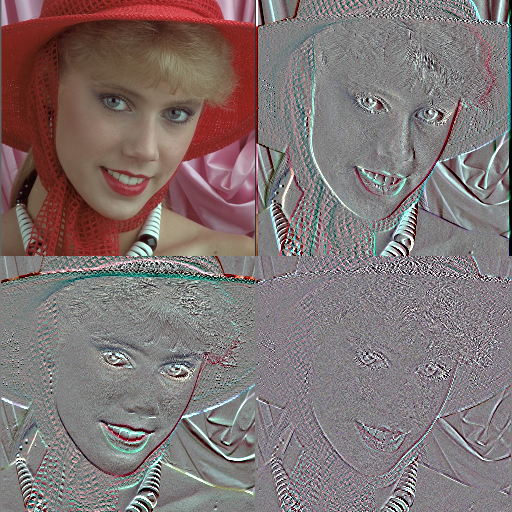
\includegraphics[width=0.90\linewidth]{methods/figures/SP_Level1.png}};

        % labels in each corner
        \node[anchor=north west, font=\medium\bfseries,
              xshift=-18pt, yshift=-4pt] at (img.north west) {LL};
        \node[anchor=north east, font=\medium\bfseries,
              xshift=18pt, yshift=-4pt] at (img.north east) {HL};
        \node[anchor=south west, font=\medium\bfseries,
              xshift=-18pt, yshift=4pt] at (img.south west) {LH};
        \node[anchor{south east}, font=\medium\bfseries,
              xshift=12pt, yshift=6pt] at (img.south east) {HH};
    \end{tikzpicture}
    \caption{One level of the S+P transform.}
    \label{fig:sp_level1}
\end{figure}

\begin{figure}[ht]
    \centering
    \begin{tikzpicture}
        \node[inner sep=0] (img)
            {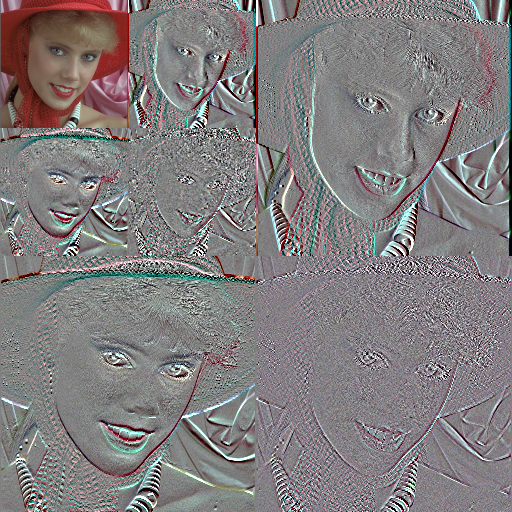
\includegraphics[width=0.90\linewidth]{methods/figures/SP_Level2.png}};

        % labels in each corner
        \node[anchor=north west, font=\medium\bfseries,
              xshift=-22pt, yshift=-4pt] at (img.north west) {LL2};
        \node[anchor=north west, font=\medium\bfseries,
              xshift=-22pt, yshift=8pt] at (img.west) {LH2};
        \node[anchor=north west, font=\medium\bfseries,
              xshift=-22pt, yshift=12pt] at (img.north) {HL2};
        \node[anchor=north west, font=\medium\bfseries,
              xshift=-22pt, yshift=8pt] at (img.center) {HH2};
        \node[anchor=north east, font=\medium\bfseries,
        \node[anchor=north east, font=\medium\bfseries,
              xshift=22pt, yshift=-4pt] at (img.north east) {HL1};
        \node[anchor=south west, font=\medium\bfseries,
              xshift=-22pt, yshift=4pt] at (img.south west) {LH1};
        \node[anchor{south east}, font=\medium\bfseries,
              xshift=12pt, yshift=6pt] at (img.south east) {HH1};
    \end{tikzpicture}
    \caption{Two levels of the S+P transform.}
    \label{fig:sp_level2}
\end{figure}

The correlation coefficient measures the normalized linear dependence between two adjacent data points, ranging from −1 to 1, with higher positive values indicating stronger similarity. Under mild correlation assumptions—in particular, when adjacent samples have correlation coefficient larger than $\tfrac{1}{3}$—S alone already reduces the average variance of the low- and highpass components relative to the original signal~\cite{said1993sp}. The P stage is specifically designed to exploit the residual correlation that remains, mainly in the highpass bands.

\subsubsection{The S+P Transform: Prediction Embedded in the Transform}

The S+P transform augments the S stage with a predictive step that operates directly on the highpass coefficients produced at each one-dimensional pass. Conceptually, we distinguish three sequences:
\begin{itemize}
    \item $s[n]$: the lowpass component after the S stage,
    \item $d_1[n]$: the intermediate highpass component (exact differences),
    \item $d[n]$: the final highpass residual after prediction.
\end{itemize}

\subsubsection{Predictor structure}

We introduce a simple notation for local lowpass differences:
\begin{equation}
    z_\ell[n] = s[n-1] - s[n],
\end{equation}
where $ \ell$ captures local gradients in the lowpass band. Following~\cite{said1993sp}, we estimate $d_1[n]$ from neighboring lowpass samples and the next highpass value $d_1[n+1]$. A generic linear estimator has the form
\begin{equation}
\begin{aligned}
\hat d_1[n] 
    &= \beta_{-1} \, z_\ell[n] 
     + \beta_0   \, z_\ell[n+1] \\
    &\quad + \beta_{+1} \, z_\ell[n+2]
     - \phi_1 \, d_1[n+1].
\end{aligned}
\end{equation}

where $\beta_{-1}, \beta_0, \beta_{+1}, \phi_1$ are predictor coefficients. Intuitively, the first three terms exploit smoothness in the lowpass band, while the last term models correlation between adjacent highpass coefficients. These coefficients were originally obtained by fitting a local linear model to natural and medical images so as to 
minimize the mean–square prediction error of $d_1[n]$ given neighboring lowpass differences and the next highpass 
sample. The fitted values for $(\beta_{-1},\beta_0,\beta_{+1},\phi_1)$ are fixed and do not depend on the image, 
allowing the transform to remain perfectly reversible prior to quantization. For our implementation we use the coefficient set
\[
\beta_{-1}=-1,\qquad \beta_0=2,\qquad \beta_{+1}=-1,\qquad \phi_1=1,
\]
which is the recommended configuration from~\cite{said1993sp}.


To preserve integer reversibility, we do not subtract $\hat{d}_1[n]$ directly. Instead, we perform a quantized correction using an integer denominator $K = 2^{k}$:
\begin{equation}
    \mathrm{pred}[n] = \left\lfloor \frac{\hat{d}_1[n]}{K} \right\rfloor,
\end{equation}
and define the residual
\begin{equation}
    d[n] = d_1[n] - \mathrm{pred}[n].
\end{equation}
The final transformed highpass component is thus $d[n]$, and $d_1[n]$ never needs to be stored explicitly beyond the prediction step.

\subsubsection{Inverse S+P and exact reconstruction}

The inverse transform proceeds in the reverse order of the forward transform. During the inverse of a one-dimensional pass, we assume that $s[n]$ and $d[n]$ are available. We reconstruct $d_1[n]$ by reapplying the same predictor in reverse:
\begin{enumerate}
    \item Visit indices in descending order $n = N/2-1, \dots, 0$, ensuring that $d_1[n+1]$ is already reconstructed when needed.
    \item For each $n$, compute the same predictor numerator using current $s[\cdot]$ and $d_1[n+1]$.
    \item Recompute $\mathrm{pred}[n] = \left\lfloor \hat{d}_1[n] / K \right\rfloor$ and add it back:
    \begin{equation}
        d_1[n] = d[n] + \mathrm{pred}[n].
    \end{equation}
\end{enumerate}
Once $d_1[n]$ is recovered for all $n$, the inverse S transform recovers the original samples $c[2n]$ and $c[2n+1]$ exactly. The crucial point is that the predictor and its quantization are perfectly reproducible during inversion, so no information is lost.

% In our implementation, we adopt a parameterization closely aligned with the ``natural image'' predictor family in~\cite{said1993sp}, but we expose $\beta_{-1}$, $\beta_0$, $\beta_{+1}$, $\phi_1$, and the shift $k$ as tunable parameters. This makes it possible to experiment with both conservative predictors (small attenuation, robust on textured images) and more aggressive ones (strong low-frequency attenuation, favorable on smooth images).
\subsubsection{Frequency-Domain Interpretation}

Although the S+P transform is defined via local integer operations, its behavior is illuminating when viewed in the frequency domain. If we ignore truncation for the sake of analysis and treat the operations as linear, the mapping from the original sequence $c[n]$ to the highpass residual $d[n]$ can be represented as a linear time-invariant filter with a frequency response $F(\mathrm{e}^{j\omega})$.

The S stage alone already suppresses low frequencies in the highpass band, but it does so relatively mildly; the resulting highpass spectrum still exhibits considerable low-frequency energy due to the piecewise-constant nature of the Haar-like filter. By embedding prediction in the transform, S+P effectively implements an additional highpass filter: the predictor attempts to explain away low-frequency variations in $d_1[n]$ using neighboring lowpass differences and adjacent highpass values. When the predictor coefficients are chosen appropriately, $|F(\mathrm{e}^{j\omega})|$ exhibits significantly stronger attenuation at low frequencies than the basic S transform.

There is, of course, a trade-off. Stronger low-frequency attenuation generally comes at the cost of some amplification in higher frequencies. For smooth, low-noise images, this trade-off is supposedly advantageous: the additional whitening reduces the variance and first-order entropy of $d[n]$, improving compressibility. For highly textured or noisy images, it may be beneficial to temper the predictor so as not to over-amplify high-frequency content. Said and Pearlman demonstrate that, in practice, a small set of carefully tuned predictors can work well across a broad range of natural and medical images~\cite{said1993sp}. 


\subsubsection{Complexity and Runtime Considerations}

From an algorithmic standpoint, the S+P transform has the same asymptotic complexity as the underlying S transform. For an image of size $W \times H$, a single S pass along rows and columns is $O(WH)$: every pixel participates in a constant number of operations. The P stage introduces only a small constant-factor overhead: each highpass coefficient requires a few extra integer operations for the predictor numerator and a single integer shift.

More explicitly:
\begin{itemize}
    \item S stage: for each pair $(c[2n], c[2n+1])$, we compute one difference and one sum with a shift, $O(1)$ per pixel.
    \item P stage: for each highpass index $n$, we access a small fixed stencil of lowpass samples and one neighboring highpass value, perform a handful of integer multiplies/adds, and one right shift by a fixed number of bits, again $O(1)$ per highpass coefficient.
\end{itemize}
Because the transform is applied recursively only to the LL subband, which shrinks by a factor of four at each level, the total work over all levels of the pyramid remains $O(WH)$. Compared to block DCT or longer-tap wavelets, S+P remains light-weight, fully in-place, and integer-only; in our pipeline measurements, entropy coding and I/O dominate total runtime.

% \subsubsection{Implementation Details in Our Pipeline}

% We now describe how we integrated the S+P transform into our C++ image-compression pipeline and highlight several design decisions that distinguish our implementation from a baseline integer Haar transform.

% \paragraph{Data model and in-place layout.} 
% Our pipeline operates on \texttt{Chunk} objects, each representing a rectangular block of a single image plane (Y, Cb, or Cr) with a contiguous data pointer and stride. The S+P core exposes a minimal interface:
% \begin{align*}
%     \texttt{forward2D(Plane plane)} \quad \text{and} \quad \texttt{inverse2D(Plane plane)},
% \end{align*}
% both of which operate in-place on the provided buffer. At each recursion level, we apply the one-dimensional forward S+P transform to all rows, then to all columns. The LL, HL, LH, and HH subbands are packed into quadrants of the same array, and we recurse only on the LL quadrant, mirroring the wavelet-style layout used by Haar.

% \paragraph{Integer arithmetic and border handling.}
% A central goal of our implementation is to preserve exact integer reversibility while being robust to a wide range of image sizes. Two technical points are worth emphasizing:
% \begin{itemize}
%     \item \textbf{Consistent floor-division for negatives.} We implement a helper \texttt{floor\_divK(x, shift)} that emulates floor-division by $2^{\text{shift}}$ for both positive and negative integers. This eliminates subtle asymmetries that arise from naive right-shifts on negative values and is critical to making the prediction and its inverse bit-exact.
%     \item \textbf{Configurable border policy.} The S+P core supports both clamping and mirror-padding at the boundaries. In our current configuration we default to clamping for simplicity, but the implementation exposes a \texttt{Border} enum so that we can experiment with symmetric extension if we wish to minimize edge artifacts in the transformed coefficients.
% \end{itemize}
% These rounding and boundary rules are more explicit than in our baseline Haar code, where edges are handled implicitly and floating-point rounding is less constrained.

% \paragraph{Stable inverse prediction at the boundaries.}
% The inverse prediction step requires reconstructing $d_1[n]$ from residuals $d[n]$ and predicted values. In the interior of the signal this is straightforward: $d_1[n+1]$ is available when computing $d_1[n]$. Near the right boundary, however, a naive closed-form expression that treats $d_1[n]$ and $d_1[n+1]$ symmetrically can fail for certain integer combinations, leading to small but catastrophic inconsistencies during reconstruction.

% To avoid this, our implementation treats boundary positions explicitly. In the interior we reuse the analytic update rule proposed in~\cite{said1993sp}. At the last highpass index, we instead solve for $d_1[n]$ via a short fixed-point iteration: we initialize a candidate $d_1[n]$ and iteratively recompute the corresponding prediction until the quantized prediction stabilizes. In practice this converges in a handful of iterations and guarantees that the forward and inverse predictions are perfectly matched, even at the edges. This design choice is unique to S+P in our pipeline and trades a negligible amount of computation at the boundary for greatly improved robustness.

% \paragraph{Comparison to a baseline Haar implementation.}
% Relative to the simple integer Haar implementation used elsewhere in the paper, the present S+P core differs in three main ways:
% \begin{itemize}
%     \item It inserts the P stage on top of the basic S transform, with the explicit goal of reducing residual correlation in the highpass bands and thus lowering their entropy.
%     \item It makes border handling explicit and configurable, rather than implicitly reusing edge pixels.
%     \item It enforces exact symmetry between forward and inverse prediction, including at the boundaries, via the fixed-point reconstruction strategy described above.
% \end{itemize}
% These changes allow us to study S+P as a drop-in alternative to the Haar transform while keeping the external interface and overall complexity nearly identical.

% \subsubsection{Quantization for the S+P Transform}

% When used in a lossless mode, the S+P transform is followed directly by entropy coding, and all coefficients are preserved exactly. For lossy compression, we introduce bandwise scalar quantization on top of the S+P coefficients. Because S+P already segregates information into subbands of differing perceptual importance (LL vs.\ HL/LH/HH), it is natural to assign different step sizes to each band.

% \paragraph{Bandwise and level-dependent parameterization.}
% We expose a small set of quantization parameters grouped in a \texttt{QuantParams} structure:
% \begin{itemize}
%     \item $q_{\mathrm{LL}}, q_{\mathrm{HL}}, q_{\mathrm{LH}}, q_{\mathrm{HH}}$: base step sizes for the four subbands,
%     \item \texttt{deadzone}: a dimensionless multiplier for the central dead-zone around zero,
%     \item \texttt{scale}: a global scale factor applied uniformly to all bands,
%     \item \texttt{level\_gamma}: a geometric multiplier applied per pyramid level.
% \end{itemize}
% From these, we compute per-level step sizes
% \begin{align}
%     q_{\mathrm{band}}^{(L)} &= \left\lfloor \texttt{scale} \cdot \mathrm{level\_factor}(L) \cdot q_{\mathrm{band}} \right\rfloor, \\
%     \mathrm{level\_factor}(L) &=
%       \begin{cases}
%         \texttt{level\_gamma}^{L} & \text{if } \texttt{level\_gamma} > 0, \\
%         1                         & \text{otherwise.}
%       \end{cases}
% \end{align}
% for each band and pyramid level $L$. In practice, we often keep LL coarsely quantized or even unquantized at the coarsest levels and allow more aggressive quantization in the HL/LH/HH bands, especially at finer scales where errors are less visually prominent. The choice of \texttt{deadzone} is made empirically and tuned based on observed rate--distortion performance rather than derived from a specific optimality criterion.

% \paragraph{Dead-zone scalar quantization.}
% Within each subband, we apply a standard dead-zone scalar quantizer. Given a coefficient $x$ and step size $\Delta$, we compute
% \begin{equation}
%     q = 
%     \begin{cases}
%       0, & |x| < \texttt{deadzone} \cdot \Delta, \\
%       \mathrm{sign}(x) \, \left\lfloor \dfrac{|x|}{\Delta} \right\rfloor, & \text{otherwise,}
%     \end{cases}
% \end{equation}
% and reconstruct via $\hat{x} = q \Delta$ during decoding. The enlarged dead-zone around zero encourages small-magnitude coefficients---especially in highpass bands---to be quantized to zero, which in turn leads to long runs of zeros that are efficiently compressed by the entropy coder.

% Because S+P already reduces the variance and entropy of the highpass residuals, we expect that competitive rate--distortion performance can be achieved with relatively simple scalar quantization. Moreover, the explicit control over band- and level-dependent step sizes gives us a clean experimental lever: we can vary $(q_{\mathrm{LL}}, q_{\mathrm{HL}}, q_{\mathrm{LH}}, q_{\mathrm{HH}})$ and \texttt{level\_gamma} to probe how S+P behaves under different operating points without modifying the transform itself.
\label{methodsec:sp}

\subsection{Quantization}
\label{methodsec:quant}
% Content for Quantization Methods subsection
% This file is included in the main conference paper via % Content for Quantization Methods subsection
% This file is included in the main conference paper via % Content for Quantization Methods subsection
% This file is included in the main conference paper via \input{QuantizationMethods}
\subsubsection{Quantization Theory}
Quantization is the lossy process of reducing the bits needed to store data by dividing  from a larger range of values to a smaller range of values. By decreasing the range used to represent the data, entropy is lowered, as multiple values pre-quantization may be mapped to one value during quantization. With this mapping being many-to-one, this operation cannot be reversed, showing that quantization is necessarily lossy. With the goal of transforms being to decrease entropy while ensuring perfect reconstruction of an image, quantization is used to further improve compression ratio beyond entropy-bound compression used in lossless algorithms, sacrificing image fidelity in the process. Fig. \ref{fig:quantization} depicts the effect of increasing levels of quantization and the associated loss of image quality, along with compression ratio of the compressed file as defined in \ref{sec:intro}.

\begin{figure}
    \centering
    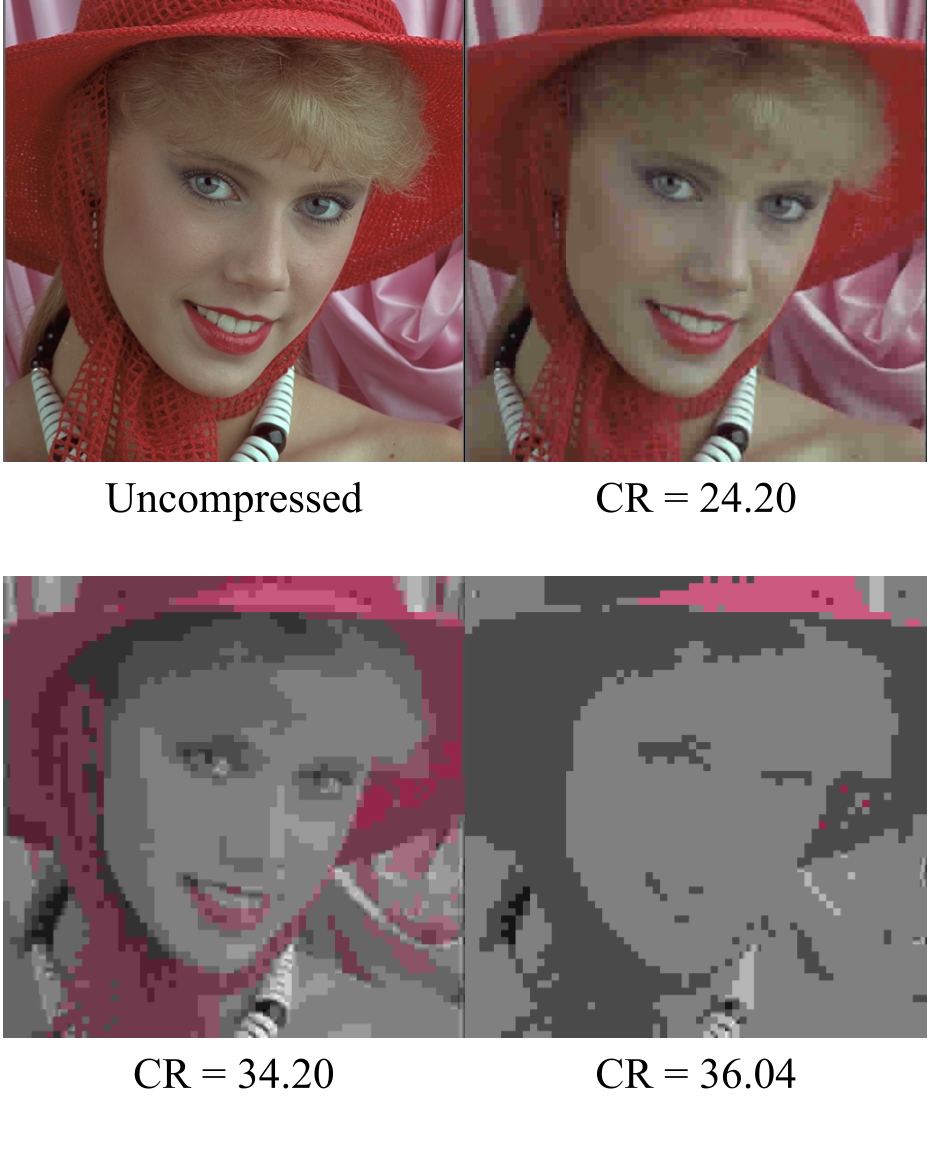
\includegraphics[width=0.8\linewidth]{methods/figures/quantizationfigure.png}
    \caption{Different levels of quantization on sample image with resulting compression ratio.}
    \label{fig:quantization}
\end{figure}

A central component to quantization is step size $\Delta$, which points to the ranges of pre-quantized values that would be quantized to one resulting value. With R representing the range of values and M the number of steps, step size is given by:
\begin{equation}
\Delta = \frac{R}{M}\label{eq}
\end{equation}
To illustrate the role of step size, consider an 8-bit signal whose values lie in the range 0–255. A step size of $\Delta = 2$ would quantize that range into $128$ steps:
\begin{equation}
2 = \frac{256}{M}\label{step_size}
\end{equation}
\begin{equation}
M = 128 = 2^{7}\label{7bits}
\end{equation}
Thus, the output symbols of this example quantizer can be represented using $7$ bits per value, before the following entropy encoding.

In our study, a relatively simple base quantization method was devised based on the JPEG Compression Standard. Quantization was applied on each chunk via division by a defined quantization matrix associated with each transform. DCT and DFT utilized a quantization matrix specified by the JPEG Compression Standard, whereas other transforms had quantization matrices calculated based on transformed data ranges.

Because the JPEG-specified quantization matrix is labeled as resulting in a 50\% reduction in quality, the quantization methods for the Haar and S+P transforms aimed to reduce the theoretical bit-representation of the image from 8 bits to 7 bits. For the Haar transform, this was done by calculating the data ranges for each quadrant of each transformed chunk and choosing the appropriate step sizes based on $M = 128$ to achieve a basic quantization matrix. A unique quantization method was created for the S+P transform. 
\subsubsection{Quantization for the S+P Transform}

For lossy compression, we introduce bandwise scalar quantization on top of the
S+P coefficients. Because S+P already segregates information into subbands of
differing perceptual importance (LL vs.\ HL/LH/HH), it is natural to assign
different step sizes to each band rather than using a uniform matrix.

\paragraph{Bandwise and level-dependent parameterization.}
Our implementation exposes a small set of quantization parameters in a
\texttt{QuantParams} structure:
\begin{itemize}
    \item $q_{\mathrm{LL}}, q_{\mathrm{HL}}, q_{\mathrm{LH}}, q_{\mathrm{HH}}$: base step sizes for the four subbands,
    \item \texttt{deadzone}: a dimensionless multiplier for the central dead-zone,
    \item \texttt{scale}: a global scale factor applied uniformly across bands,
    \item \texttt{level\_gamma}: a geometric multiplier applied per pyramid level.
\end{itemize}

From these we compute per-level step sizes
\begin{align}
    q_{\mathrm{band}}^{(L)} &= \left\lfloor
        \texttt{scale} \cdot \mathrm{level\_factor}(L) \cdot q_{\mathrm{band}}
    \right\rfloor, \\
    \mathrm{level\_factor}(L) &=
      \begin{cases}
        \texttt{level\_gamma}^{L}, & \text{if } \texttt{level\_gamma} > 0, \\
        1, & \text{otherwise}.
      \end{cases}
\end{align}
for each band and level $L$. In practice, the LL band at coarse levels is often
left unquantized or lightly quantized, while higher-frequency bands (HL/LH/HH)
receive progressively larger steps, reflecting their lower perceptual weight.
Because all S+P coefficients are integers, these step sizes are also rounded to
integers, which can further couple quantizer behavior to the underlying
coefficient distribution. As in the Haar case, the choice of \texttt{deadzone}
is made empirically and tuned based on observed rate--distortion behavior.

\paragraph{Dead-zone scalar quantization.}
Within each subband, we apply a standard dead-zone scalar quantizer. Given a
coefficient $x$ and step size $\Delta$, we compute
\begin{equation}
    q =
    \begin{cases}
      0, & |x| < \texttt{deadzone}\cdot\Delta, \\
      \mathrm{sign}(x)\,\left\lfloor \dfrac{|x|}{\Delta} \right\rfloor,
      & \text{otherwise,}
    \end{cases}
\end{equation}
and reconstruct via $\hat{x} = q\Delta$ during decoding. The enlarged dead-zone
encourages small-magnitude coefficients—especially in the highpass bands—to be
quantized to zero, producing longer zero-runs that the entropy coder can
compress efficiently.

Because the S+P transform tends to reduce the variance and entropy of its
highpass residuals, relatively simple scalar quantizers can still achieve a wide
range of operating points. Moreover, the explicit bandwise and level-dependent
parameters allow us to adjust $(q_{\mathrm{LL}}, q_{\mathrm{HL}},
q_{\mathrm{LH}}, q_{\mathrm{HH}})$ and \texttt{level\_gamma} to probe different
rate--distortion regimes without modifying the transform itself.

\subsubsection{Quantization Theory}
Quantization is the lossy process of reducing the bits needed to store data by dividing  from a larger range of values to a smaller range of values. By decreasing the range used to represent the data, entropy is lowered, as multiple values pre-quantization may be mapped to one value during quantization. With this mapping being many-to-one, this operation cannot be reversed, showing that quantization is necessarily lossy. With the goal of transforms being to decrease entropy while ensuring perfect reconstruction of an image, quantization is used to further improve compression ratio beyond entropy-bound compression used in lossless algorithms, sacrificing image fidelity in the process. Fig. \ref{fig:quantization} depicts the effect of increasing levels of quantization and the associated loss of image quality, along with compression ratio of the compressed file as defined in \ref{sec:intro}.

\begin{figure}
    \centering
    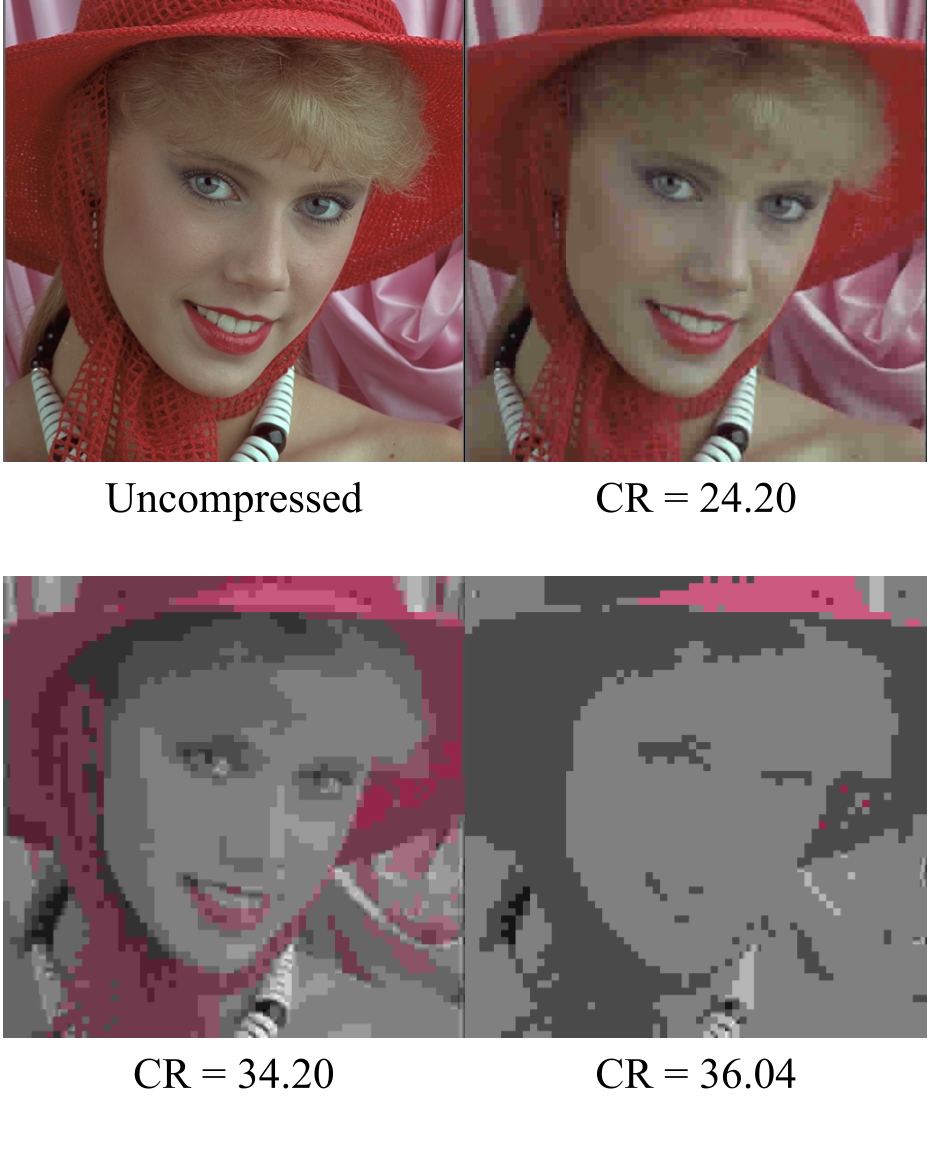
\includegraphics[width=0.8\linewidth]{methods/figures/quantizationfigure.png}
    \caption{Different levels of quantization on sample image with resulting compression ratio.}
    \label{fig:quantization}
\end{figure}

A central component to quantization is step size $\Delta$, which points to the ranges of pre-quantized values that would be quantized to one resulting value. With R representing the range of values and M the number of steps, step size is given by:
\begin{equation}
\Delta = \frac{R}{M}\label{eq}
\end{equation}
To illustrate the role of step size, consider an 8-bit signal whose values lie in the range 0–255. A step size of $\Delta = 2$ would quantize that range into $128$ steps:
\begin{equation}
2 = \frac{256}{M}\label{step_size}
\end{equation}
\begin{equation}
M = 128 = 2^{7}\label{7bits}
\end{equation}
Thus, the output symbols of this example quantizer can be represented using $7$ bits per value, before the following entropy encoding.

In our study, a relatively simple base quantization method was devised based on the JPEG Compression Standard. Quantization was applied on each chunk via division by a defined quantization matrix associated with each transform. DCT and DFT utilized a quantization matrix specified by the JPEG Compression Standard, whereas other transforms had quantization matrices calculated based on transformed data ranges.

Because the JPEG-specified quantization matrix is labeled as resulting in a 50\% reduction in quality, the quantization methods for the Haar and S+P transforms aimed to reduce the theoretical bit-representation of the image from 8 bits to 7 bits. For the Haar transform, this was done by calculating the data ranges for each quadrant of each transformed chunk and choosing the appropriate step sizes based on $M = 128$ to achieve a basic quantization matrix. A unique quantization method was created for the S+P transform. 
\subsubsection{Quantization for the S+P Transform}

For lossy compression, we introduce bandwise scalar quantization on top of the
S+P coefficients. Because S+P already segregates information into subbands of
differing perceptual importance (LL vs.\ HL/LH/HH), it is natural to assign
different step sizes to each band rather than using a uniform matrix.

\paragraph{Bandwise and level-dependent parameterization.}
Our implementation exposes a small set of quantization parameters in a
\texttt{QuantParams} structure:
\begin{itemize}
    \item $q_{\mathrm{LL}}, q_{\mathrm{HL}}, q_{\mathrm{LH}}, q_{\mathrm{HH}}$: base step sizes for the four subbands,
    \item \texttt{deadzone}: a dimensionless multiplier for the central dead-zone,
    \item \texttt{scale}: a global scale factor applied uniformly across bands,
    \item \texttt{level\_gamma}: a geometric multiplier applied per pyramid level.
\end{itemize}

From these we compute per-level step sizes
\begin{align}
    q_{\mathrm{band}}^{(L)} &= \left\lfloor
        \texttt{scale} \cdot \mathrm{level\_factor}(L) \cdot q_{\mathrm{band}}
    \right\rfloor, \\
    \mathrm{level\_factor}(L) &=
      \begin{cases}
        \texttt{level\_gamma}^{L}, & \text{if } \texttt{level\_gamma} > 0, \\
        1, & \text{otherwise}.
      \end{cases}
\end{align}
for each band and level $L$. In practice, the LL band at coarse levels is often
left unquantized or lightly quantized, while higher-frequency bands (HL/LH/HH)
receive progressively larger steps, reflecting their lower perceptual weight.
Because all S+P coefficients are integers, these step sizes are also rounded to
integers, which can further couple quantizer behavior to the underlying
coefficient distribution. As in the Haar case, the choice of \texttt{deadzone}
is made empirically and tuned based on observed rate--distortion behavior.

\paragraph{Dead-zone scalar quantization.}
Within each subband, we apply a standard dead-zone scalar quantizer. Given a
coefficient $x$ and step size $\Delta$, we compute
\begin{equation}
    q =
    \begin{cases}
      0, & |x| < \texttt{deadzone}\cdot\Delta, \\
      \mathrm{sign}(x)\,\left\lfloor \dfrac{|x|}{\Delta} \right\rfloor,
      & \text{otherwise,}
    \end{cases}
\end{equation}
and reconstruct via $\hat{x} = q\Delta$ during decoding. The enlarged dead-zone
encourages small-magnitude coefficients—especially in the highpass bands—to be
quantized to zero, producing longer zero-runs that the entropy coder can
compress efficiently.

Because the S+P transform tends to reduce the variance and entropy of its
highpass residuals, relatively simple scalar quantizers can still achieve a wide
range of operating points. Moreover, the explicit bandwise and level-dependent
parameters allow us to adjust $(q_{\mathrm{LL}}, q_{\mathrm{HL}},
q_{\mathrm{LH}}, q_{\mathrm{HH}})$ and \texttt{level\_gamma} to probe different
rate--distortion regimes without modifying the transform itself.

\subsubsection{Quantization Theory}
Quantization is the lossy process of reducing the bits needed to store data by dividing  from a larger range of values to a smaller range of values. By decreasing the range used to represent the data, entropy is lowered, as multiple values pre-quantization may be mapped to one value during quantization. With this mapping being many-to-one, this operation cannot be reversed, showing that quantization is necessarily lossy. With the goal of transforms being to decrease entropy while ensuring perfect reconstruction of an image, quantization is used to further improve compression ratio beyond entropy-bound compression used in lossless algorithms, sacrificing image fidelity in the process. Fig. \ref{fig:quantization} depicts the effect of increasing levels of quantization and the associated loss of image quality, along with compression ratio of the compressed file as defined in \ref{sec:intro}.

\begin{figure}
    \centering
    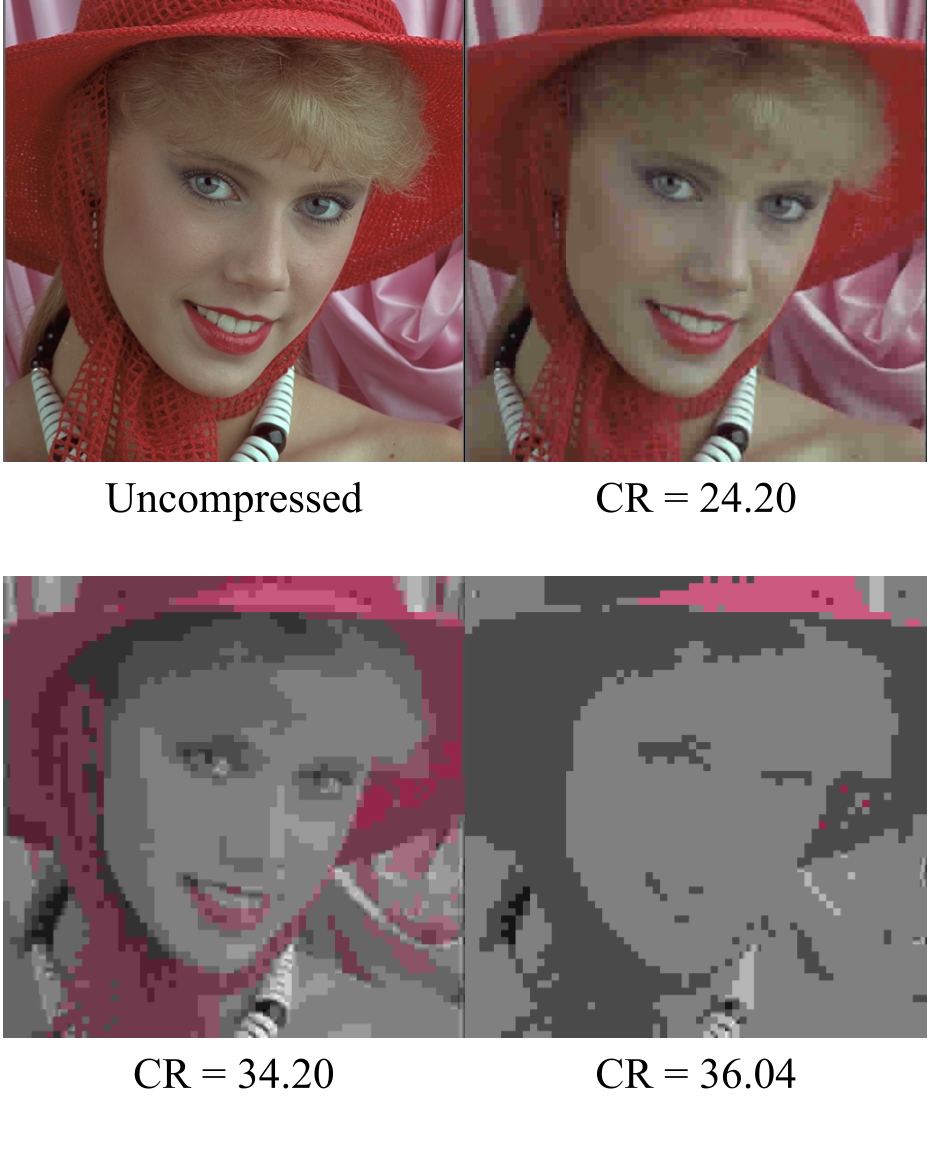
\includegraphics[width=0.8\linewidth]{methods/figures/quantizationfigure.png}
    \caption{Different levels of quantization on sample image with resulting compression ratio.}
    \label{fig:quantization}
\end{figure}

A central component to quantization is step size $\Delta$, which points to the ranges of pre-quantized values that would be quantized to one resulting value. With R representing the range of values and M the number of steps, step size is given by:
\begin{equation}
\Delta = \frac{R}{M}\label{eq}
\end{equation}
To illustrate the role of step size, consider an 8-bit signal whose values lie in the range 0–255. A step size of $\Delta = 2$ would quantize that range into $128$ steps:
\begin{equation}
2 = \frac{256}{M}\label{step_size}
\end{equation}
\begin{equation}
M = 128 = 2^{7}\label{7bits}
\end{equation}
Thus, the output symbols of this example quantizer can be represented using $7$ bits per value, before the following entropy encoding.

In our study, a relatively simple base quantization method was devised based on the JPEG Compression Standard. Quantization was applied on each chunk via division by a defined quantization matrix associated with each transform. DCT and DFT utilized a quantization matrix specified by the JPEG Compression Standard, whereas other transforms had quantization matrices calculated based on transformed data ranges.

Because the JPEG-specified quantization matrix is labeled as resulting in a 50\% reduction in quality, the quantization methods for the Haar and S+P transforms aimed to reduce the theoretical bit-representation of the image from 8 bits to 7 bits. For the Haar transform, this was done by calculating the data ranges for each quadrant of each transformed chunk and choosing the appropriate step sizes based on $M = 128$ to achieve a basic quantization matrix. A unique quantization method was created for the S+P transform. 
\subsubsection{Quantization for the S+P Transform}

For lossy compression, we introduce bandwise scalar quantization on top of the
S+P coefficients. Because S+P already segregates information into subbands of
differing perceptual importance (LL vs.\ HL/LH/HH), it is natural to assign
different step sizes to each band rather than using a uniform matrix.

\paragraph{Bandwise and level-dependent parameterization.}
Our implementation exposes a small set of quantization parameters in a
\texttt{QuantParams} structure:
\begin{itemize}
    \item $q_{\mathrm{LL}}, q_{\mathrm{HL}}, q_{\mathrm{LH}}, q_{\mathrm{HH}}$: base step sizes for the four subbands,
    \item \texttt{deadzone}: a dimensionless multiplier for the central dead-zone,
    \item \texttt{scale}: a global scale factor applied uniformly across bands,
    \item \texttt{level\_gamma}: a geometric multiplier applied per pyramid level.
\end{itemize}

From these we compute per-level step sizes
\begin{align}
    q_{\mathrm{band}}^{(L)} &= \left\lfloor
        \texttt{scale} \cdot \mathrm{level\_factor}(L) \cdot q_{\mathrm{band}}
    \right\rfloor, \\
    \mathrm{level\_factor}(L) &=
      \begin{cases}
        \texttt{level\_gamma}^{L}, & \text{if } \texttt{level\_gamma} > 0, \\
        1, & \text{otherwise}.
      \end{cases}
\end{align}
for each band and level $L$. In practice, the LL band at coarse levels is often
left unquantized or lightly quantized, while higher-frequency bands (HL/LH/HH)
receive progressively larger steps, reflecting their lower perceptual weight.
Because all S+P coefficients are integers, these step sizes are also rounded to
integers, which can further couple quantizer behavior to the underlying
coefficient distribution. As in the Haar case, the choice of \texttt{deadzone}
is made empirically and tuned based on observed rate--distortion behavior.

\paragraph{Dead-zone scalar quantization.}
Within each subband, we apply a standard dead-zone scalar quantizer. Given a
coefficient $x$ and step size $\Delta$, we compute
\begin{equation}
    q =
    \begin{cases}
      0, & |x| < \texttt{deadzone}\cdot\Delta, \\
      \mathrm{sign}(x)\,\left\lfloor \dfrac{|x|}{\Delta} \right\rfloor,
      & \text{otherwise,}
    \end{cases}
\end{equation}
and reconstruct via $\hat{x} = q\Delta$ during decoding. The enlarged dead-zone
encourages small-magnitude coefficients—especially in the highpass bands—to be
quantized to zero, producing longer zero-runs that the entropy coder can
compress efficiently.

Because the S+P transform tends to reduce the variance and entropy of its
highpass residuals, relatively simple scalar quantizers can still achieve a wide
range of operating points. Moreover, the explicit bandwise and level-dependent
parameters allow us to adjust $(q_{\mathrm{LL}}, q_{\mathrm{HL}},
q_{\mathrm{LH}}, q_{\mathrm{HH}})$ and \texttt{level\_gamma} to probe different
rate--distortion regimes without modifying the transform itself.


\subsection{Entropy Coding}
\label{methodsec:entropy}
Entropy coding is a class of compression algorithms to occur last in the pipeline. These algorithms are given their name because their effectiveness is bounded by the entropy of incoming data. In the JPEG Compression Standard, a combination of Run-Length Encoding (RLE) and Differential Pulse Code Modulation (DPCM) is used, whose results are then fed into a Huffman Coder. The areas where these algorithms are used can be observed in Fig. \ref{fig:entropyjpeg}, with DPCM being used on the top left value of each chunk across all chunks in a channel (highlighted in green), and RLE being used on the remaining values in a single chunk, with the order in which values are encoded showed by the purple arrow.

Run-Length Encoding, as the name suggests, takes advantage of "runs" of data, storing the number of time a certain value or group of values repeats rather than storing every single repetition. In the case of the JPEG standard, RLE is used to group runs of zeroes in the AC components of DCT together, which appear in the data as a result of heavy quantization of DCT's high-frequency coefficients. So, each piece of data is encoded as a pair of integers, with the first being the number of preceding zeroes (up to 15) and the second being the following non-zero number (or a zero if there are 15 preceding zeroes). As an example, the string of values
\begin{equation*}
0,0,0,4,0,12,0,0,8,2.
\end{equation*}
would be encoded to
\begin{equation*}
(3,4);(1,12);(2,8);(0,2).
\end{equation*}
\begin{figure}
    \centering
    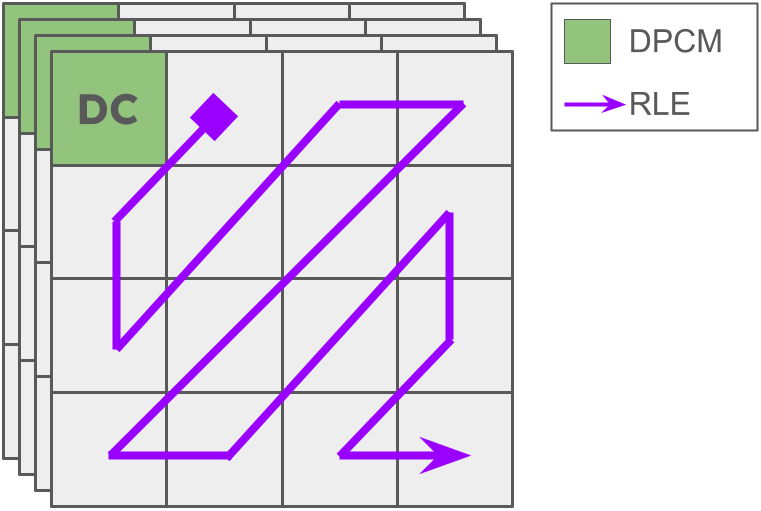
\includegraphics[width=0.8\linewidth]{methods/figures/dctentropyencode.png}
    \caption{Visual of different entropy encoding algorithms used for DCT as specified by JPEG Compression Standard.}
    \label{fig:entropyjpeg}
\end{figure}
While RLE is used for AC components, DPCM is used for DC components. At its core, DPCM is purely a differential coding algorithm, meaning it stores only the differences between values rather than the actual values themselves. This algorithm is most effective when adjacent values are correlated, which is the case for DC coefficients of adjacent image chunks (see "why images section"). By storing solely the differences between values, DPCM effectively stores values from the derivative function of the unencoded data, provided the unencoded data is correlated by some function itself. Thus, the efficiency of this algorithm depends much on the hope that the entropy of the derivative function is lower than that of the original function. Of course, to make data reconstruction possible, the first original value is stored, similarly to how integral calculation requires the constant $C$. To reconstruct the data, the differences are added to the first original value in sequence. For some sequence $[x]$ with difference sequence $[d]$:
\begin{equation}
\begin{split}
d_0 & = x_0 \\
d_1 & = x_1 - x_0 \\
d_{n} & = x_{n} - x_{n-1}
\end{split}
\end{equation}
and for reconstruction:
\begin{equation}
\begin{split}
x_0 & = d_0 \\
x_1 & = x_0 + d_1 \\
x_n & = x_{n-1} + d_n
\end{split}
\end{equation}

Related to DPCM is predictive coding, which uses previous values to predict future values and stores the difference between the actual value and the predicted value, known as prediction error. In cases when the data is highly correlated, predictions can be very accurate, causing the prediction error to be even smaller than differences calculated using DPCM, lowering entropy even further. Because of this, DPCM was substituted out for a linear predictive coder in this project pipeline. Similarly to DPCM, given some sequence $[x]$, we have predicted sequence $[p]$, with difference sequence $[d]$, where the difference sequence is stored in final data:
\begin{equation}
\begin{split}
p_n & = f(x_{n-1}, x_{n-2},...,x_{n-k}) \\
d_{n} & = x_{n} - p_n
\end{split}
\end{equation}
where function $f()$ is a linear regression model using $k$ previous values.

Luca
% Content for Huffman Coding Methods subsection
% This file is included in the main conference paper via % Content for Huffman Coding Methods subsection
% This file is included in the main conference paper via % Content for Huffman Coding Methods subsection
% This file is included in the main conference paper via \input{HuffmanMethods}

\subsubsection{Huffman Coding}

Huffman coding is an entropy encoding algorithm that serves a crucial role in the final stage of image compression pipelines. The purpose of Huffman coding is to assign variable-length binary codes to symbols based on their frequency of occurrence, with more frequent symbols receiving shorter codes and less frequent symbols receiving longer codes. This approach enables efficient representation of data by reducing the average number of bits required to encode each symbol.

In the context of image compression, Huffman coding is particularly useful because it can achieve near-optimal compression when the symbol frequencies are known. While the transform coding steps (such as DWT, DCT, and DFT) and quantization all aim at reducing the entropy of the image data by concentrating energy and removing redundancy, these steps alone do not actually compress the data if written out directly. Even after these transformations, the data still requires 8 bits per channel per pixel to represent each value. Huffman coding addresses this limitation by exploiting the non-uniform distribution of values in the transformed and quantized data, allowing frequently occurring values to be represented with fewer bits and less frequent values with more bits. This results in a reduction of the total number of bits needed to represent the data in a near-optimal way, at least when comparing to character representation with knowledge only of the character frequencies.


\subsubsection{Huffman Coding}

Huffman coding is an entropy encoding algorithm that serves a crucial role in the final stage of image compression pipelines. The purpose of Huffman coding is to assign variable-length binary codes to symbols based on their frequency of occurrence, with more frequent symbols receiving shorter codes and less frequent symbols receiving longer codes. This approach enables efficient representation of data by reducing the average number of bits required to encode each symbol.

In the context of image compression, Huffman coding is particularly useful because it can achieve near-optimal compression when the symbol frequencies are known. While the transform coding steps (such as DWT, DCT, and DFT) and quantization all aim at reducing the entropy of the image data by concentrating energy and removing redundancy, these steps alone do not actually compress the data if written out directly. Even after these transformations, the data still requires 8 bits per channel per pixel to represent each value. Huffman coding addresses this limitation by exploiting the non-uniform distribution of values in the transformed and quantized data, allowing frequently occurring values to be represented with fewer bits and less frequent values with more bits. This results in a reduction of the total number of bits needed to represent the data in a near-optimal way, at least when comparing to character representation with knowledge only of the character frequencies.


\subsubsection{Huffman Coding}

Huffman coding is an entropy encoding algorithm that serves a crucial role in the final stage of image compression pipelines. The purpose of Huffman coding is to assign variable-length binary codes to symbols based on their frequency of occurrence, with more frequent symbols receiving shorter codes and less frequent symbols receiving longer codes. This approach enables efficient representation of data by reducing the average number of bits required to encode each symbol.

In the context of image compression, Huffman coding is particularly useful because it can achieve near-optimal compression when the symbol frequencies are known. While the transform coding steps (such as DWT, DCT, and DFT) and quantization all aim at reducing the entropy of the image data by concentrating energy and removing redundancy, these steps alone do not actually compress the data if written out directly. Even after these transformations, the data still requires 8 bits per channel per pixel to represent each value. Huffman coding addresses this limitation by exploiting the non-uniform distribution of values in the transformed and quantized data, allowing frequently occurring values to be represented with fewer bits and less frequent values with more bits. This results in a reduction of the total number of bits needed to represent the data in a near-optimal way, at least when comparing to character representation with knowledge only of the character frequencies.


\section{Results}
\label{sec:results}

\subsection{Experimental Setup}
% Content for Experimental Setup subsection
% This file is included in the main conference paper via % Content for Experimental Setup subsection
% This file is included in the main conference paper via % Content for Experimental Setup subsection
% This file is included in the main conference paper via \input{ExperimentalSetup}

To compare each transform, we chose 4 unique datasets all with different types of images. Sample images for all of the datasets can be seen in Fig. \ref{fig:datasetsamples}.
\begin{enumerate}
    \item \textbf{Kodak} - Includes general pictures of people and objects. We included this to test how each transform performed on normal images.
    \item \textbf{Aerial Images} - As the name suggests, contains images taken from the air of large sections of landscape. We expected many transforms like Haar and S+P to do well on these images because of their consistent global structure, 
    \item \textbf{Textures} - The inverse of Aerial Images, this includes close-up textures of a variety of surfaces and materials. This dataset is interesting because it includes some images with good global consistency, but also many images with much more sporadic textures that vary greatly even at a small scale.
    \item \textbf{Icons} - This includes low-resolution images of a variety of various digital icons. We chose this to test since the sharp edges and transitions in color challenge the transforms, especially those like DCT and DFT.
\end{enumerate}

\begin{figure}[!h] % [!h] is a common placement modifier (here, "force here if possible")
    \centering
    % --- Top Left Image (Subfigure a) ---
    \begin{subfigure}[b]{0.22\textwidth} % [b] aligns the subfigure baseline; 0.45\textwidth controls the width
        \centering
        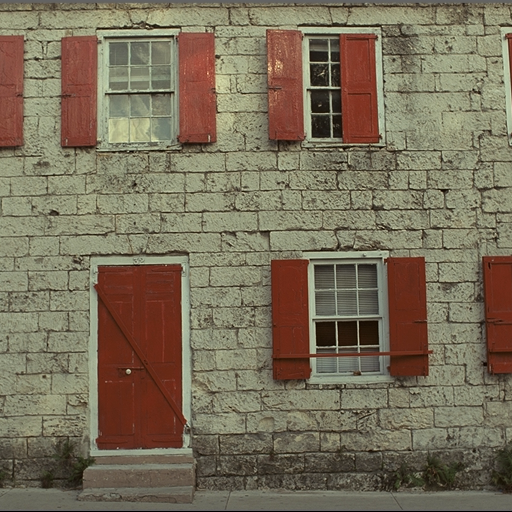
\includegraphics[width=\textwidth]{results/sample_images/kodak.png} % Replace image1.jpg with your file
        \caption{Sample \textbf{Kodak} image}
        \label{fig:kodakimg}
    \end{subfigure}
    \hfill % Adds horizontal space between the first two subfigures
    % --- Top Right Image (Subfigure b) ---
    \begin{subfigure}[b]{0.22\textwidth}
        \centering
        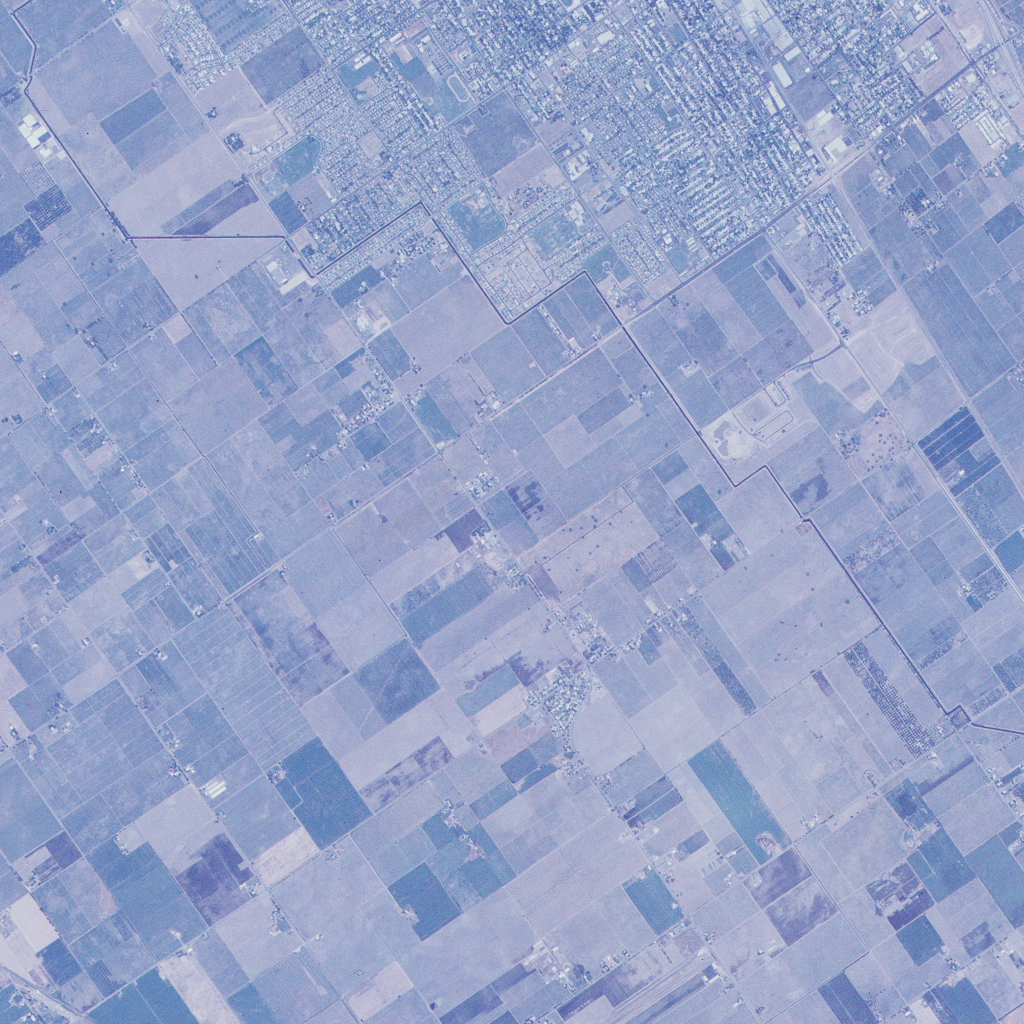
\includegraphics[width=\textwidth]{results/sample_images/aerial.png} % Replace image2.png with your file
        \caption{Sample \textbf{Aerial} image}
        \label{fig:aerialimg}
    \end{subfigure}
    
    \vspace{1em} % Adds vertical space between the top and bottom rows
    
    % --- Bottom Left Image (Subfigure c) ---
    \begin{subfigure}[b]{0.22\textwidth}
        \centering
        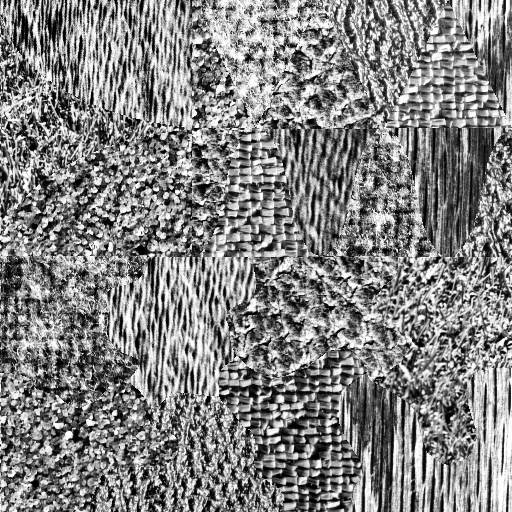
\includegraphics[width=\textwidth]{results/sample_images/texture.png} % Replace image3.eps with your file
        \caption{Sample \textbf{Texture} image}
        \label{fig:textureimg}
    \end{subfigure}
    \hfill
    % --- Bottom Right Image (Subfigure d) ---
    \begin{subfigure}[b]{0.22\textwidth}
        \centering
        
\includegraphics[width=\textwidth]{results/sample_images/icon.png} % Replace image4.gif with your file
        \caption{Sample \textbf{Icon} image}
        \label{fig:iconimg}
    \end{subfigure}
    
    % --- Main Caption for the entire 2x2 grid ---
    \caption{A sample image from each of the 4 datasets.}
    \label{fig:datasetsamples}
\end{figure}



To compare each transform, we chose 4 unique datasets all with different types of images. Sample images for all of the datasets can be seen in Fig. \ref{fig:datasetsamples}.
\begin{enumerate}
    \item \textbf{Kodak} - Includes general pictures of people and objects. We included this to test how each transform performed on normal images.
    \item \textbf{Aerial Images} - As the name suggests, contains images taken from the air of large sections of landscape. We expected many transforms like Haar and S+P to do well on these images because of their consistent global structure, 
    \item \textbf{Textures} - The inverse of Aerial Images, this includes close-up textures of a variety of surfaces and materials. This dataset is interesting because it includes some images with good global consistency, but also many images with much more sporadic textures that vary greatly even at a small scale.
    \item \textbf{Icons} - This includes low-resolution images of a variety of various digital icons. We chose this to test since the sharp edges and transitions in color challenge the transforms, especially those like DCT and DFT.
\end{enumerate}

\begin{figure}[!h] % [!h] is a common placement modifier (here, "force here if possible")
    \centering
    % --- Top Left Image (Subfigure a) ---
    \begin{subfigure}[b]{0.22\textwidth} % [b] aligns the subfigure baseline; 0.45\textwidth controls the width
        \centering
        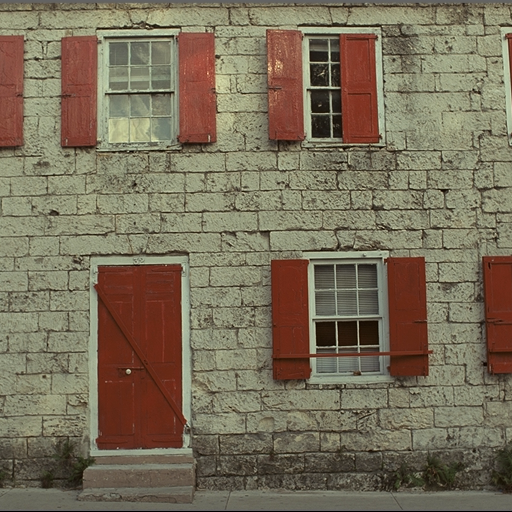
\includegraphics[width=\textwidth]{results/sample_images/kodak.png} % Replace image1.jpg with your file
        \caption{Sample \textbf{Kodak} image}
        \label{fig:kodakimg}
    \end{subfigure}
    \hfill % Adds horizontal space between the first two subfigures
    % --- Top Right Image (Subfigure b) ---
    \begin{subfigure}[b]{0.22\textwidth}
        \centering
        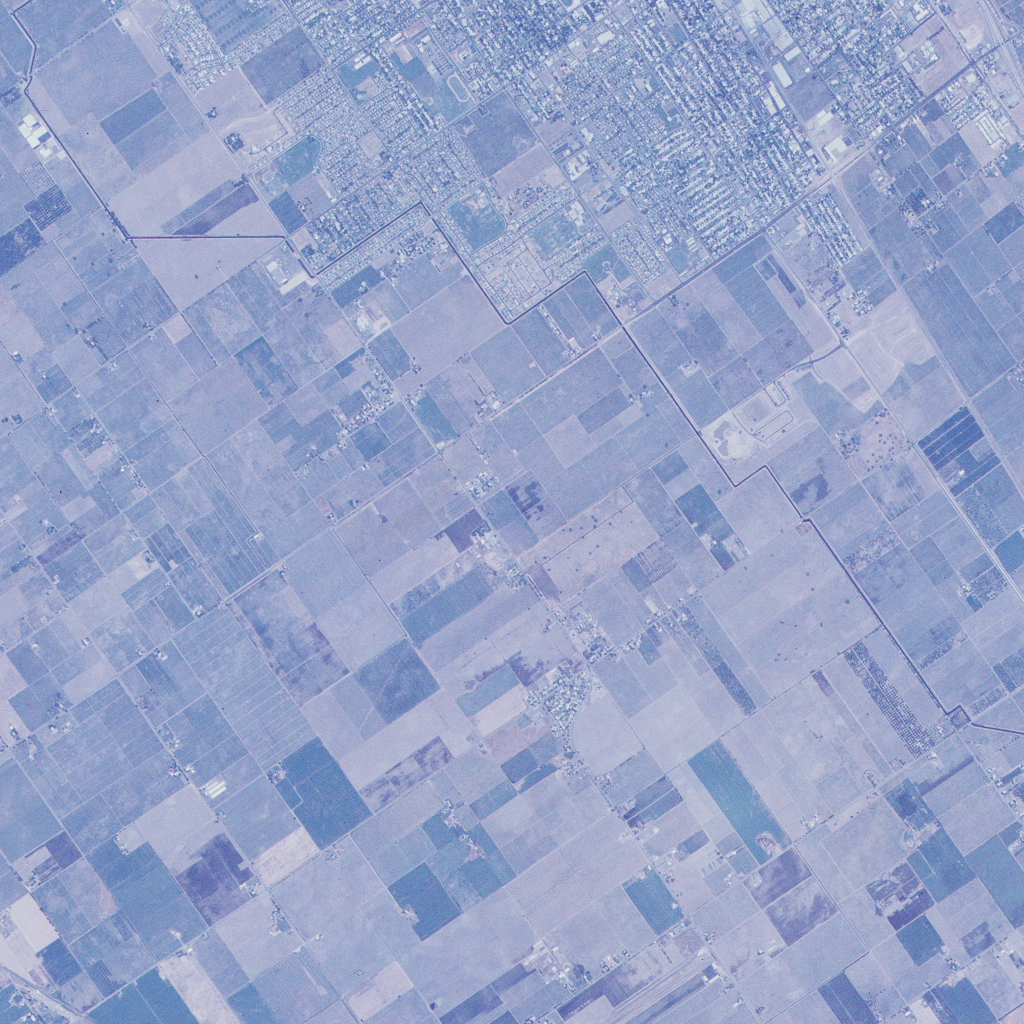
\includegraphics[width=\textwidth]{results/sample_images/aerial.png} % Replace image2.png with your file
        \caption{Sample \textbf{Aerial} image}
        \label{fig:aerialimg}
    \end{subfigure}
    
    \vspace{1em} % Adds vertical space between the top and bottom rows
    
    % --- Bottom Left Image (Subfigure c) ---
    \begin{subfigure}[b]{0.22\textwidth}
        \centering
        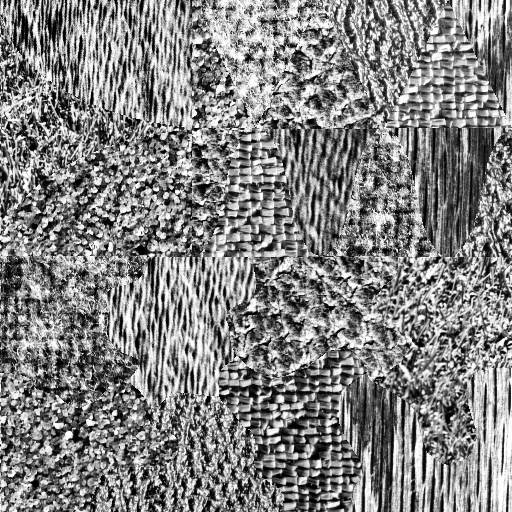
\includegraphics[width=\textwidth]{results/sample_images/texture.png} % Replace image3.eps with your file
        \caption{Sample \textbf{Texture} image}
        \label{fig:textureimg}
    \end{subfigure}
    \hfill
    % --- Bottom Right Image (Subfigure d) ---
    \begin{subfigure}[b]{0.22\textwidth}
        \centering
        
\includegraphics[width=\textwidth]{results/sample_images/icon.png} % Replace image4.gif with your file
        \caption{Sample \textbf{Icon} image}
        \label{fig:iconimg}
    \end{subfigure}
    
    % --- Main Caption for the entire 2x2 grid ---
    \caption{A sample image from each of the 4 datasets.}
    \label{fig:datasetsamples}
\end{figure}



To compare each transform, we chose 4 unique datasets all with different types of images. Sample images for all of the datasets can be seen in Fig. \ref{fig:datasetsamples}.
\begin{enumerate}
    \item \textbf{Kodak} - Includes general pictures of people and objects. We included this to test how each transform performed on normal images.
    \item \textbf{Aerial Images} - As the name suggests, contains images taken from the air of large sections of landscape. We expected many transforms like Haar and S+P to do well on these images because of their consistent global structure, 
    \item \textbf{Textures} - The inverse of Aerial Images, this includes close-up textures of a variety of surfaces and materials. This dataset is interesting because it includes some images with good global consistency, but also many images with much more sporadic textures that vary greatly even at a small scale.
    \item \textbf{Icons} - This includes low-resolution images of a variety of various digital icons. We chose this to test since the sharp edges and transitions in color challenge the transforms, especially those like DCT and DFT.
\end{enumerate}

\begin{figure}[!h] % [!h] is a common placement modifier (here, "force here if possible")
    \centering
    % --- Top Left Image (Subfigure a) ---
    \begin{subfigure}[b]{0.22\textwidth} % [b] aligns the subfigure baseline; 0.45\textwidth controls the width
        \centering
        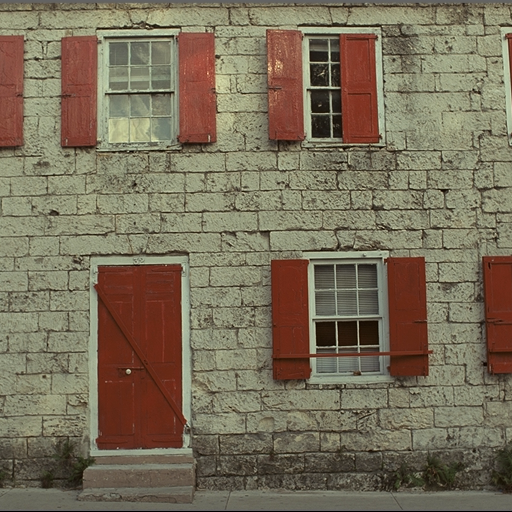
\includegraphics[width=\textwidth]{results/sample_images/kodak.png} % Replace image1.jpg with your file
        \caption{Sample \textbf{Kodak} image}
        \label{fig:kodakimg}
    \end{subfigure}
    \hfill % Adds horizontal space between the first two subfigures
    % --- Top Right Image (Subfigure b) ---
    \begin{subfigure}[b]{0.22\textwidth}
        \centering
        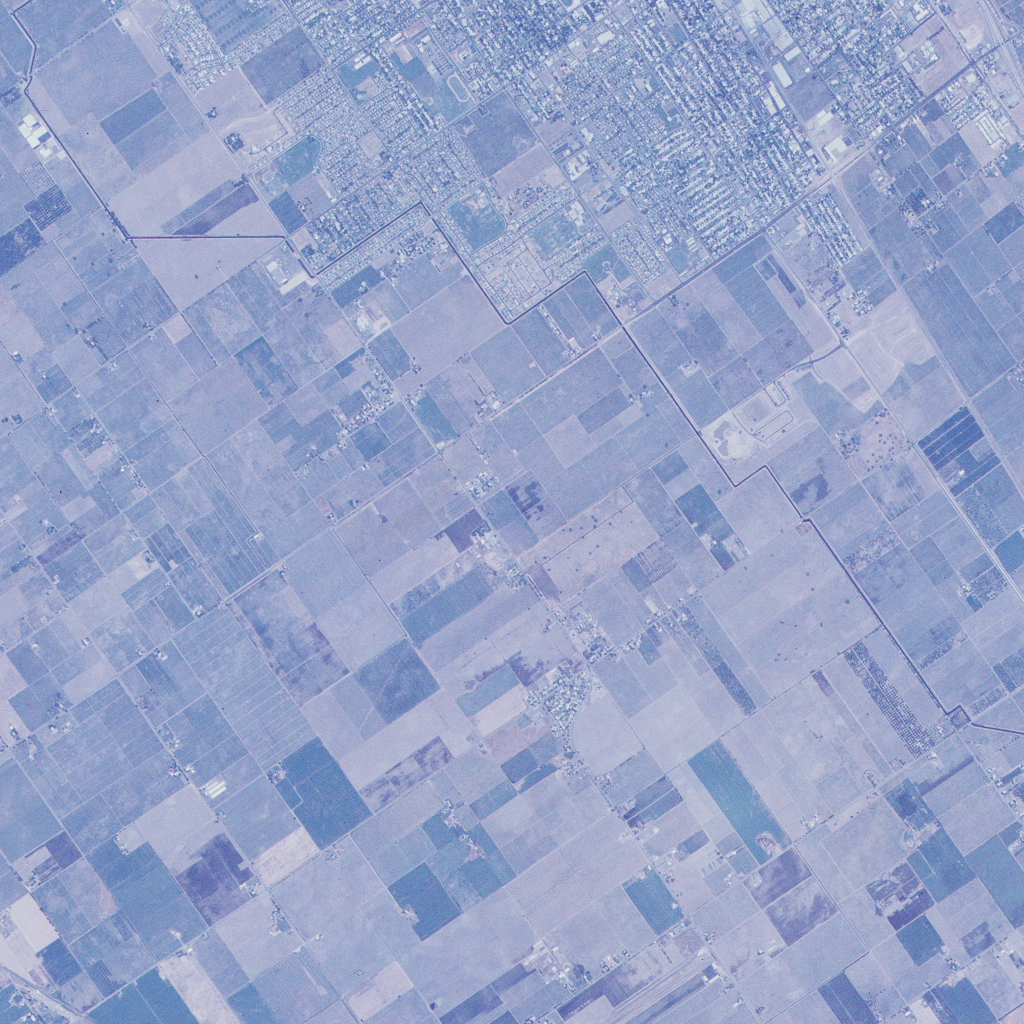
\includegraphics[width=\textwidth]{results/sample_images/aerial.png} % Replace image2.png with your file
        \caption{Sample \textbf{Aerial} image}
        \label{fig:aerialimg}
    \end{subfigure}
    
    \vspace{1em} % Adds vertical space between the top and bottom rows
    
    % --- Bottom Left Image (Subfigure c) ---
    \begin{subfigure}[b]{0.22\textwidth}
        \centering
        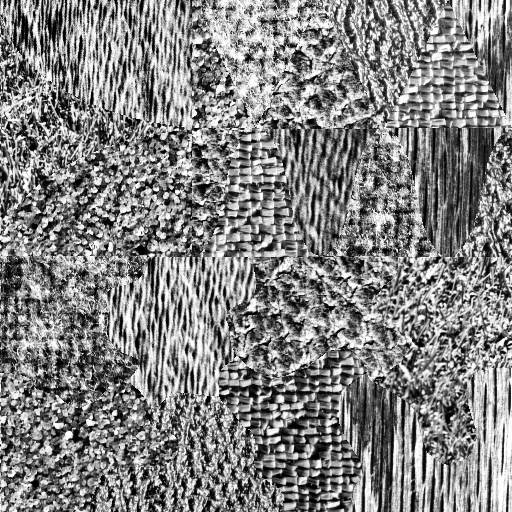
\includegraphics[width=\textwidth]{results/sample_images/texture.png} % Replace image3.eps with your file
        \caption{Sample \textbf{Texture} image}
        \label{fig:textureimg}
    \end{subfigure}
    \hfill
    % --- Bottom Right Image (Subfigure d) ---
    \begin{subfigure}[b]{0.22\textwidth}
        \centering
        
\includegraphics[width=\textwidth]{results/sample_images/icon.png} % Replace image4.gif with your file
        \caption{Sample \textbf{Icon} image}
        \label{fig:iconimg}
    \end{subfigure}
    
    % --- Main Caption for the entire 2x2 grid ---
    \caption{A sample image from each of the 4 datasets.}
    \label{fig:datasetsamples}
\end{figure}



\subsection{Metrics}
To evaluate the behavior of each transform within our compression pipeline, we
report several standard metrics drawn from image coding. These metrics quantify
both reconstruction fidelity and the effectiveness of our bitstream reduction
steps.

\paragraph{Mean Squared Error (MSE).}
Given an original image $I$ and its reconstruction $\hat{I}$, the MSE is
\begin{equation}
    \mathrm{MSE}
    = \frac{1}{N} \sum_{i=1}^{N} (I_i - \hat{I}_i)^2,
\end{equation}
where $N$ is the number of pixels. Lower MSE indicates a reconstruction closer
to the original.

\paragraph{Peak Signal-to-Noise Ratio (PSNR).}
PSNR provides a logarithmic measure of fidelity, defined as
\begin{equation}
    \mathrm{PSNR}
    = 10 \log_{10}\!\left(\frac{255^2}{\mathrm{MSE}}\right) \ \mathrm{dB},
\end{equation}
assuming 8-bit images. Higher PSNR corresponds to higher reconstruction
quality. We use PSNR as the primary distortion metric in all rate–distortion
plots.

\paragraph{Compression Ratio (CR).}
As a reminder, we define the compression ratio as
\[
\mathrm{CR} = \frac{\text{uncompressed size}}{\text{compressed size}}.
\]
Unless otherwise noted, all CR values in the rate--distortion plots refer to the 
final bitstream after entropy coding. For completeness, we also report the
pre-entropy (“direct”) CR in one diagnostic figure to examine how much gain each
transform receives from the entropy coder.

We will also continue to use Shannon's definition of entropy discussed in Section \ref{sec:lit review}. It gives an accurate picture of how well each transform successfully decorrelated the input image.

\medskip
Together, these metrics provide the basis for the rate–distortion evaluations
reported in Section \ref{sec:results}.
\label{resultssec:metrics}

\subsection{Collective Results}
\label{resultssec:col}
% Content for Collective Results subsection
% This file is included in the main conference paper via % Content for Collective Results subsection
% This file is included in the main conference paper via % Content for Collective Results subsection
% This file is included in the main conference paper via \input{CollectiveResults}
\begin{figure}
    \centering
    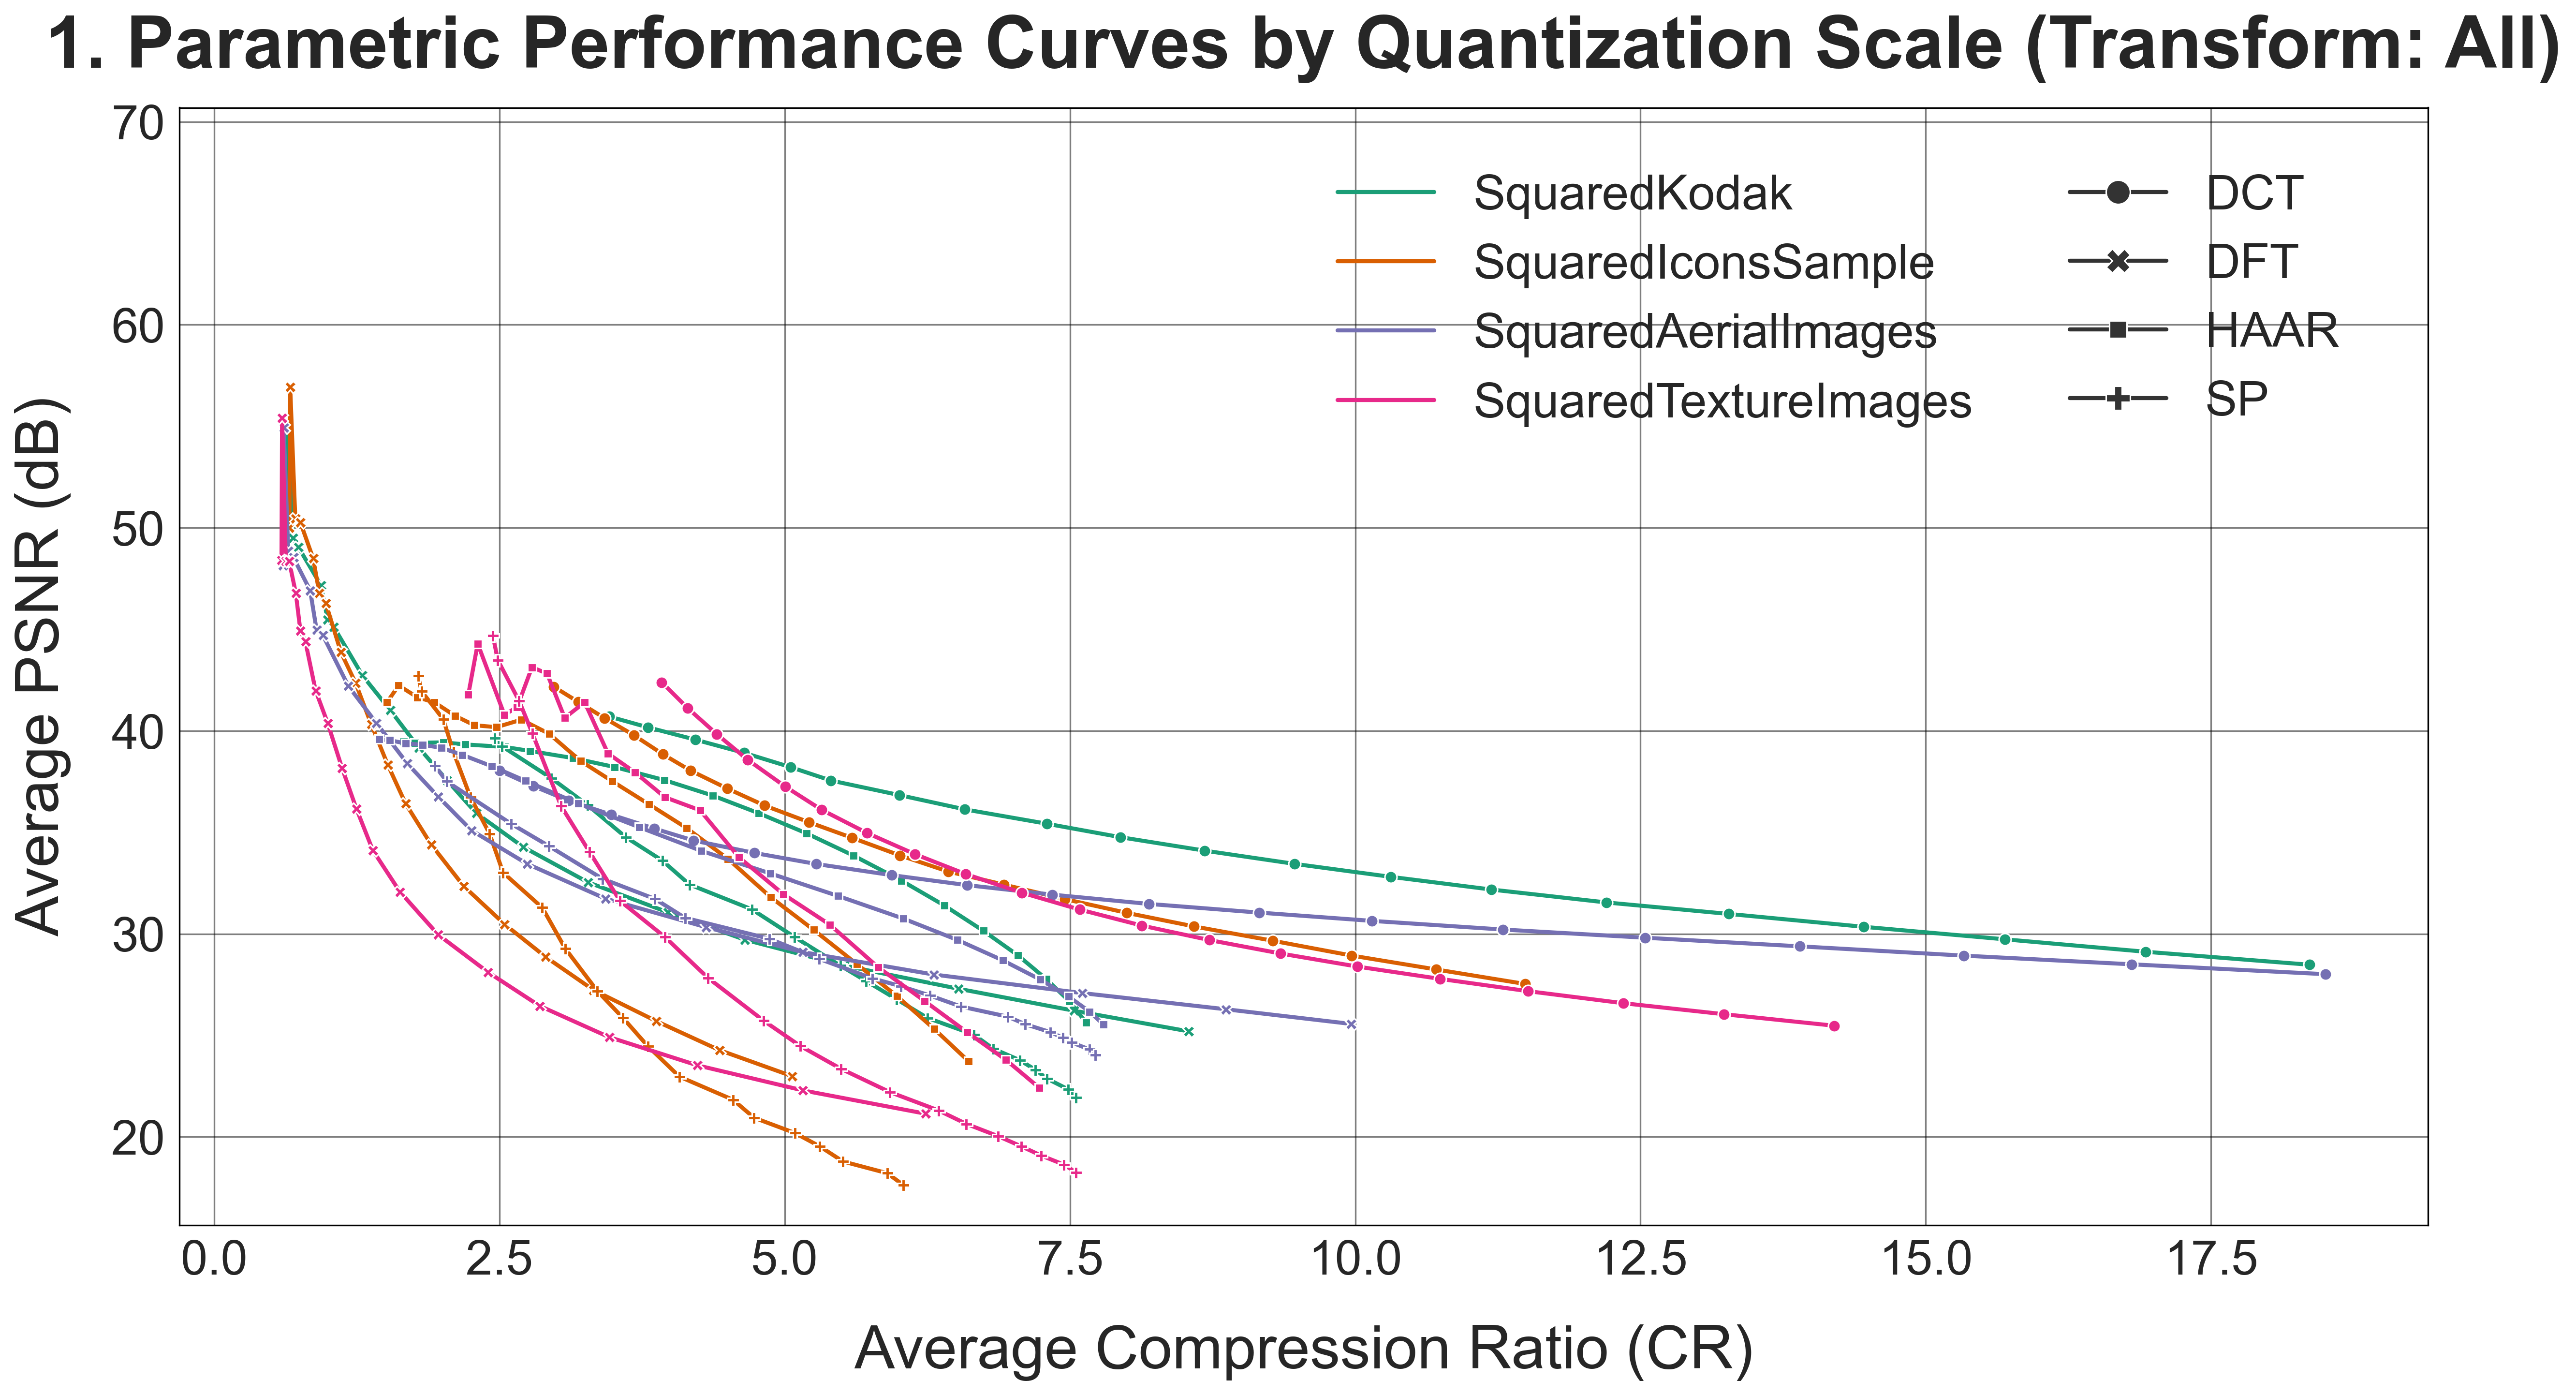
\includegraphics[width=1\linewidth]{results/plots/plot_1_parametric_curve_All.png}
    \caption{Compressed image similarity based on compression ratio by transform and dataset.}
    \label{fig:parametricAll}
\end{figure}

Firstly, as shown in fig. \ref{fig:parametricAll}, all transforms' had their quality of compressed images compared against compression ratio. Quality of compressed images, measured by the similarity between compressed and original image, or PSNR (db), is much higher for DCT, colored in blue, than all other transforms at all compression levels, with DCT additionally reaching higher compression levels than any other transform. Fig. \ref{fig:effectEntropyCoding} explores compression ratio by transform, with each box per transform representing compression ratio data with or without entropy coding used. For DCT and DFT, entropy coding generally increases compression ratio, with significant increases to the highest compression ratios achieved. On the other hand, Haar and SP see a flat decrease in compression ratio when entropy coding is used.

\begin{figure}
    \centering
    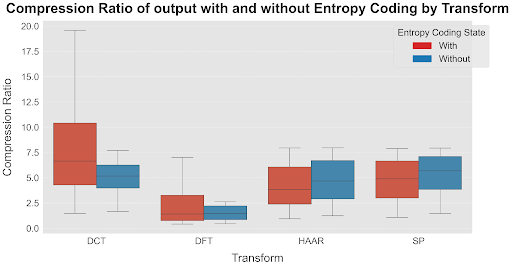
\includegraphics[width=1\linewidth]{results/plots/huffmancomparison.png}
    \caption{Effect of entropy encoding on compression ratio for all transforms}
    \label{fig:effectEntropyCoding}
\end{figure}


\begin{figure}
    \centering
    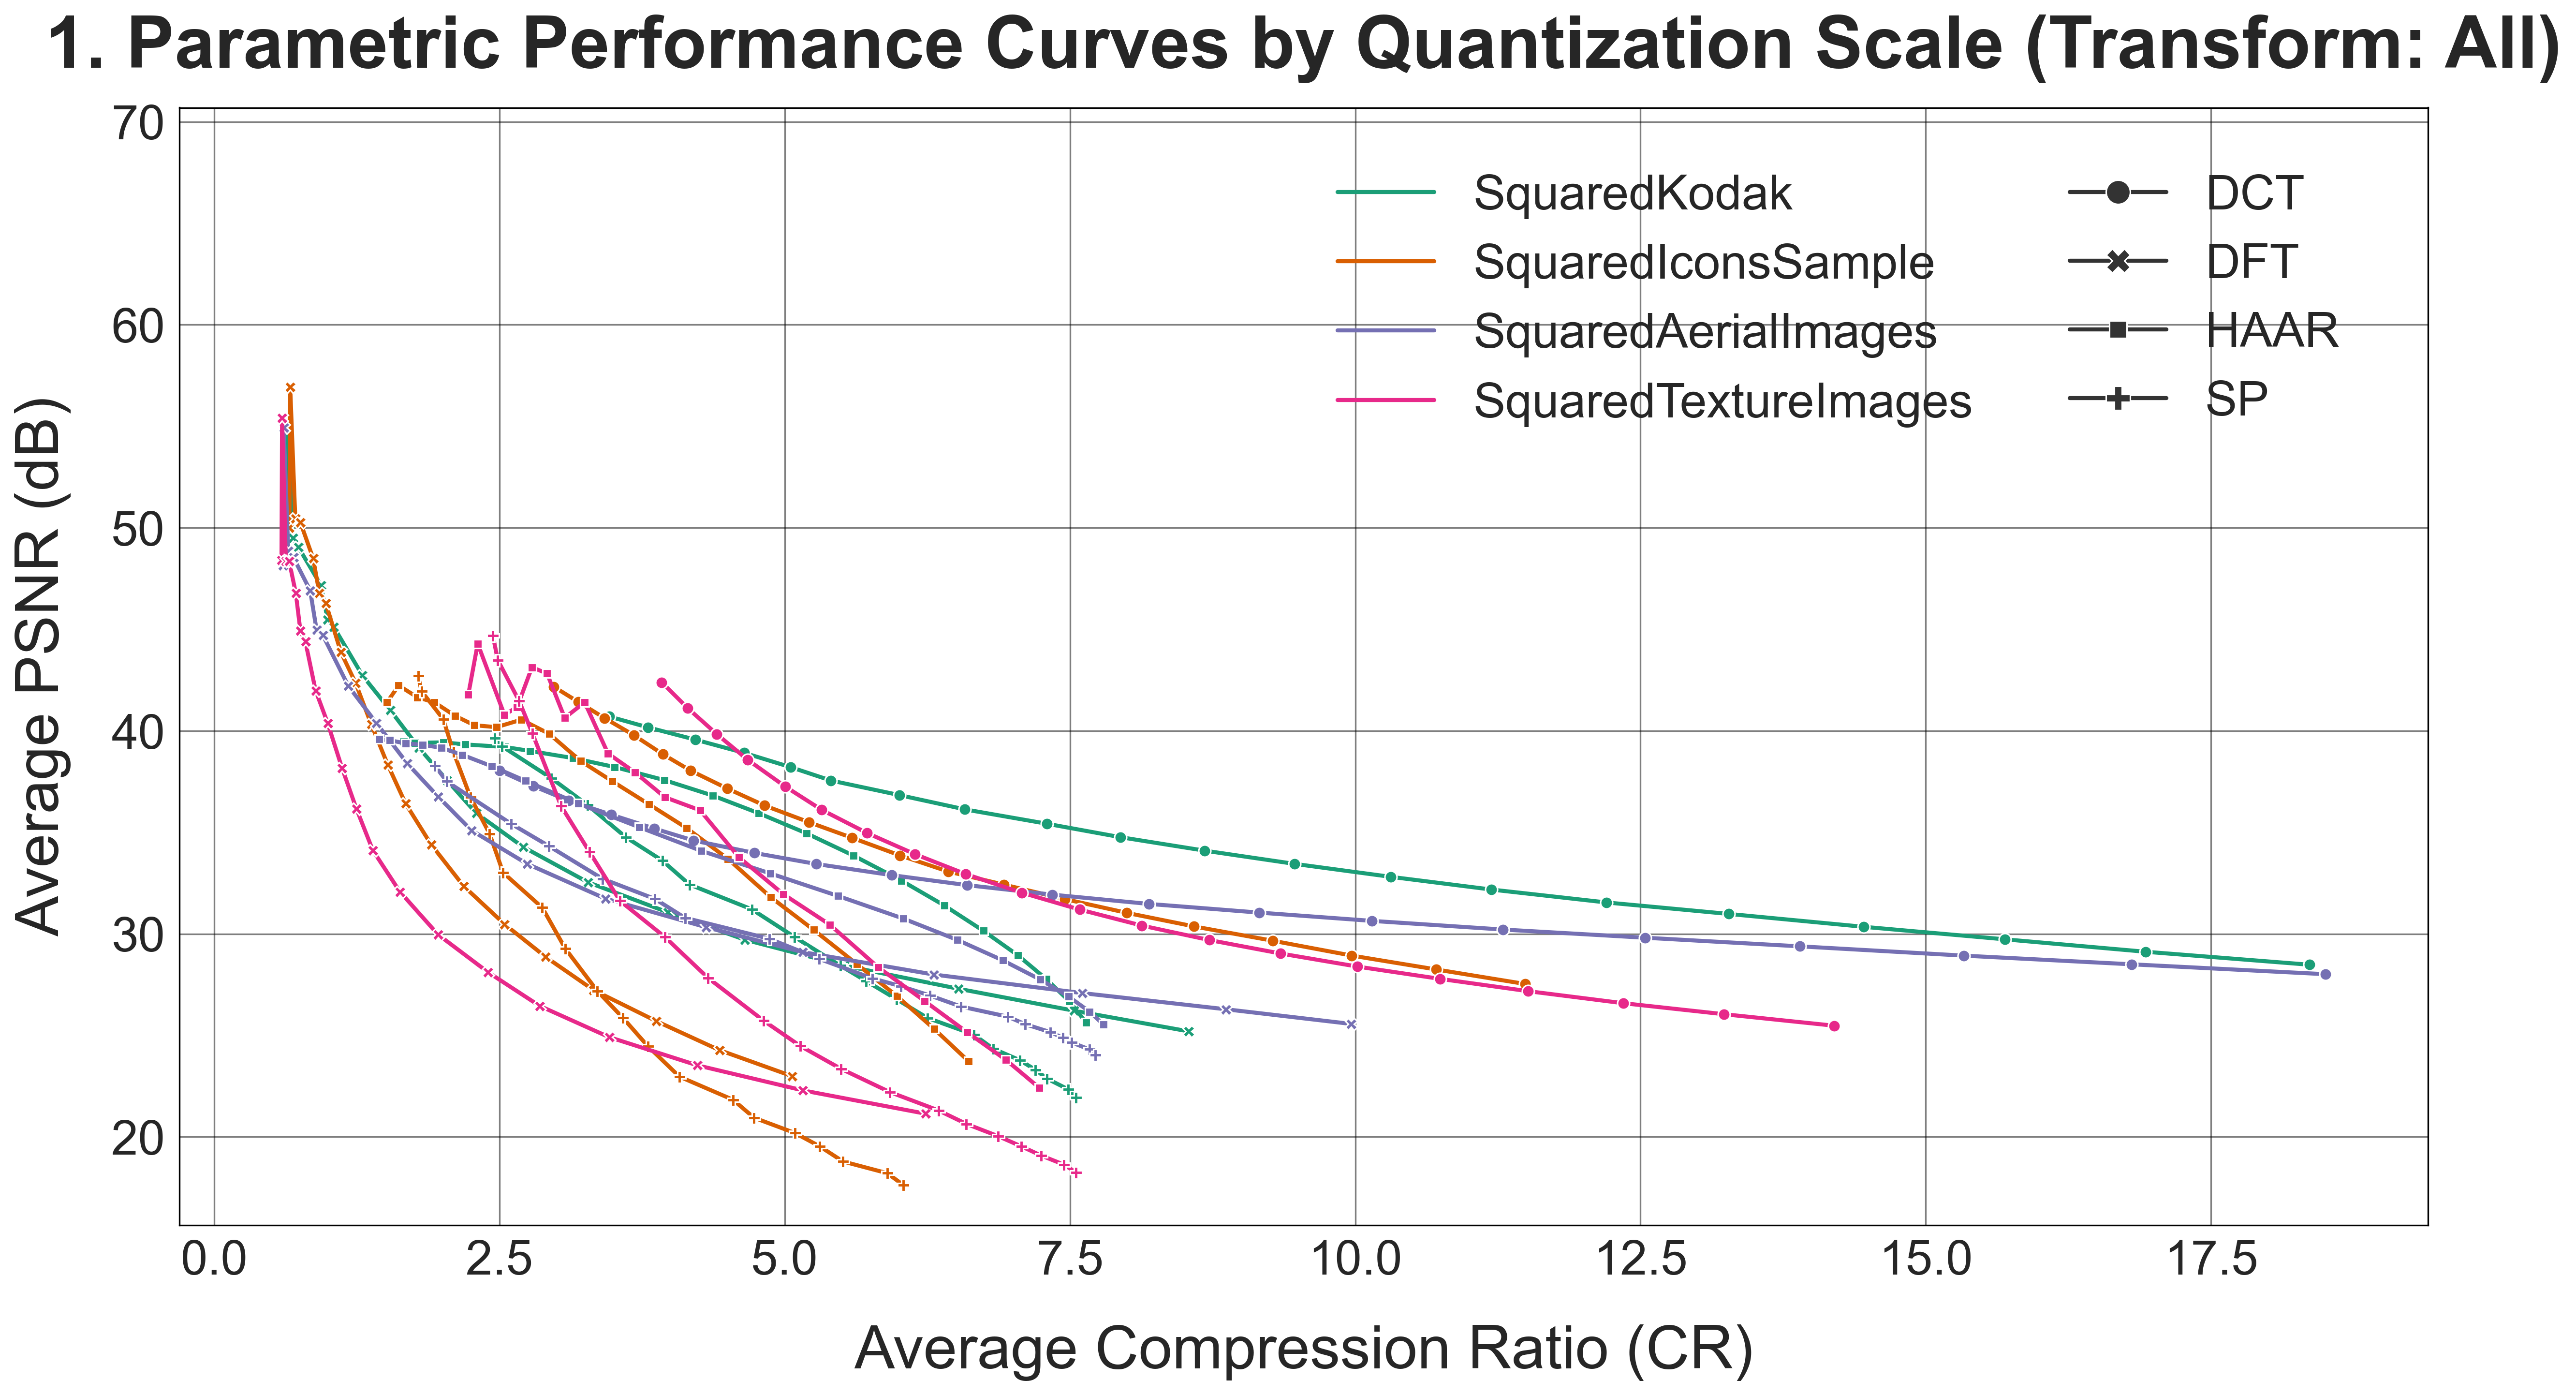
\includegraphics[width=1\linewidth]{results/plots/plot_1_parametric_curve_All.png}
    \caption{Compressed image similarity based on compression ratio by transform and dataset.}
    \label{fig:parametricAll}
\end{figure}

Firstly, as shown in fig. \ref{fig:parametricAll}, all transforms' had their quality of compressed images compared against compression ratio. Quality of compressed images, measured by the similarity between compressed and original image, or PSNR (db), is much higher for DCT, colored in blue, than all other transforms at all compression levels, with DCT additionally reaching higher compression levels than any other transform. Fig. \ref{fig:effectEntropyCoding} explores compression ratio by transform, with each box per transform representing compression ratio data with or without entropy coding used. For DCT and DFT, entropy coding generally increases compression ratio, with significant increases to the highest compression ratios achieved. On the other hand, Haar and SP see a flat decrease in compression ratio when entropy coding is used.

\begin{figure}
    \centering
    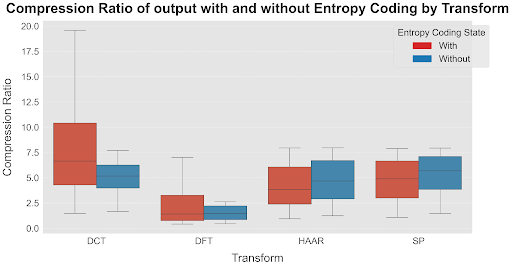
\includegraphics[width=1\linewidth]{results/plots/huffmancomparison.png}
    \caption{Effect of entropy encoding on compression ratio for all transforms}
    \label{fig:effectEntropyCoding}
\end{figure}


\begin{figure}
    \centering
    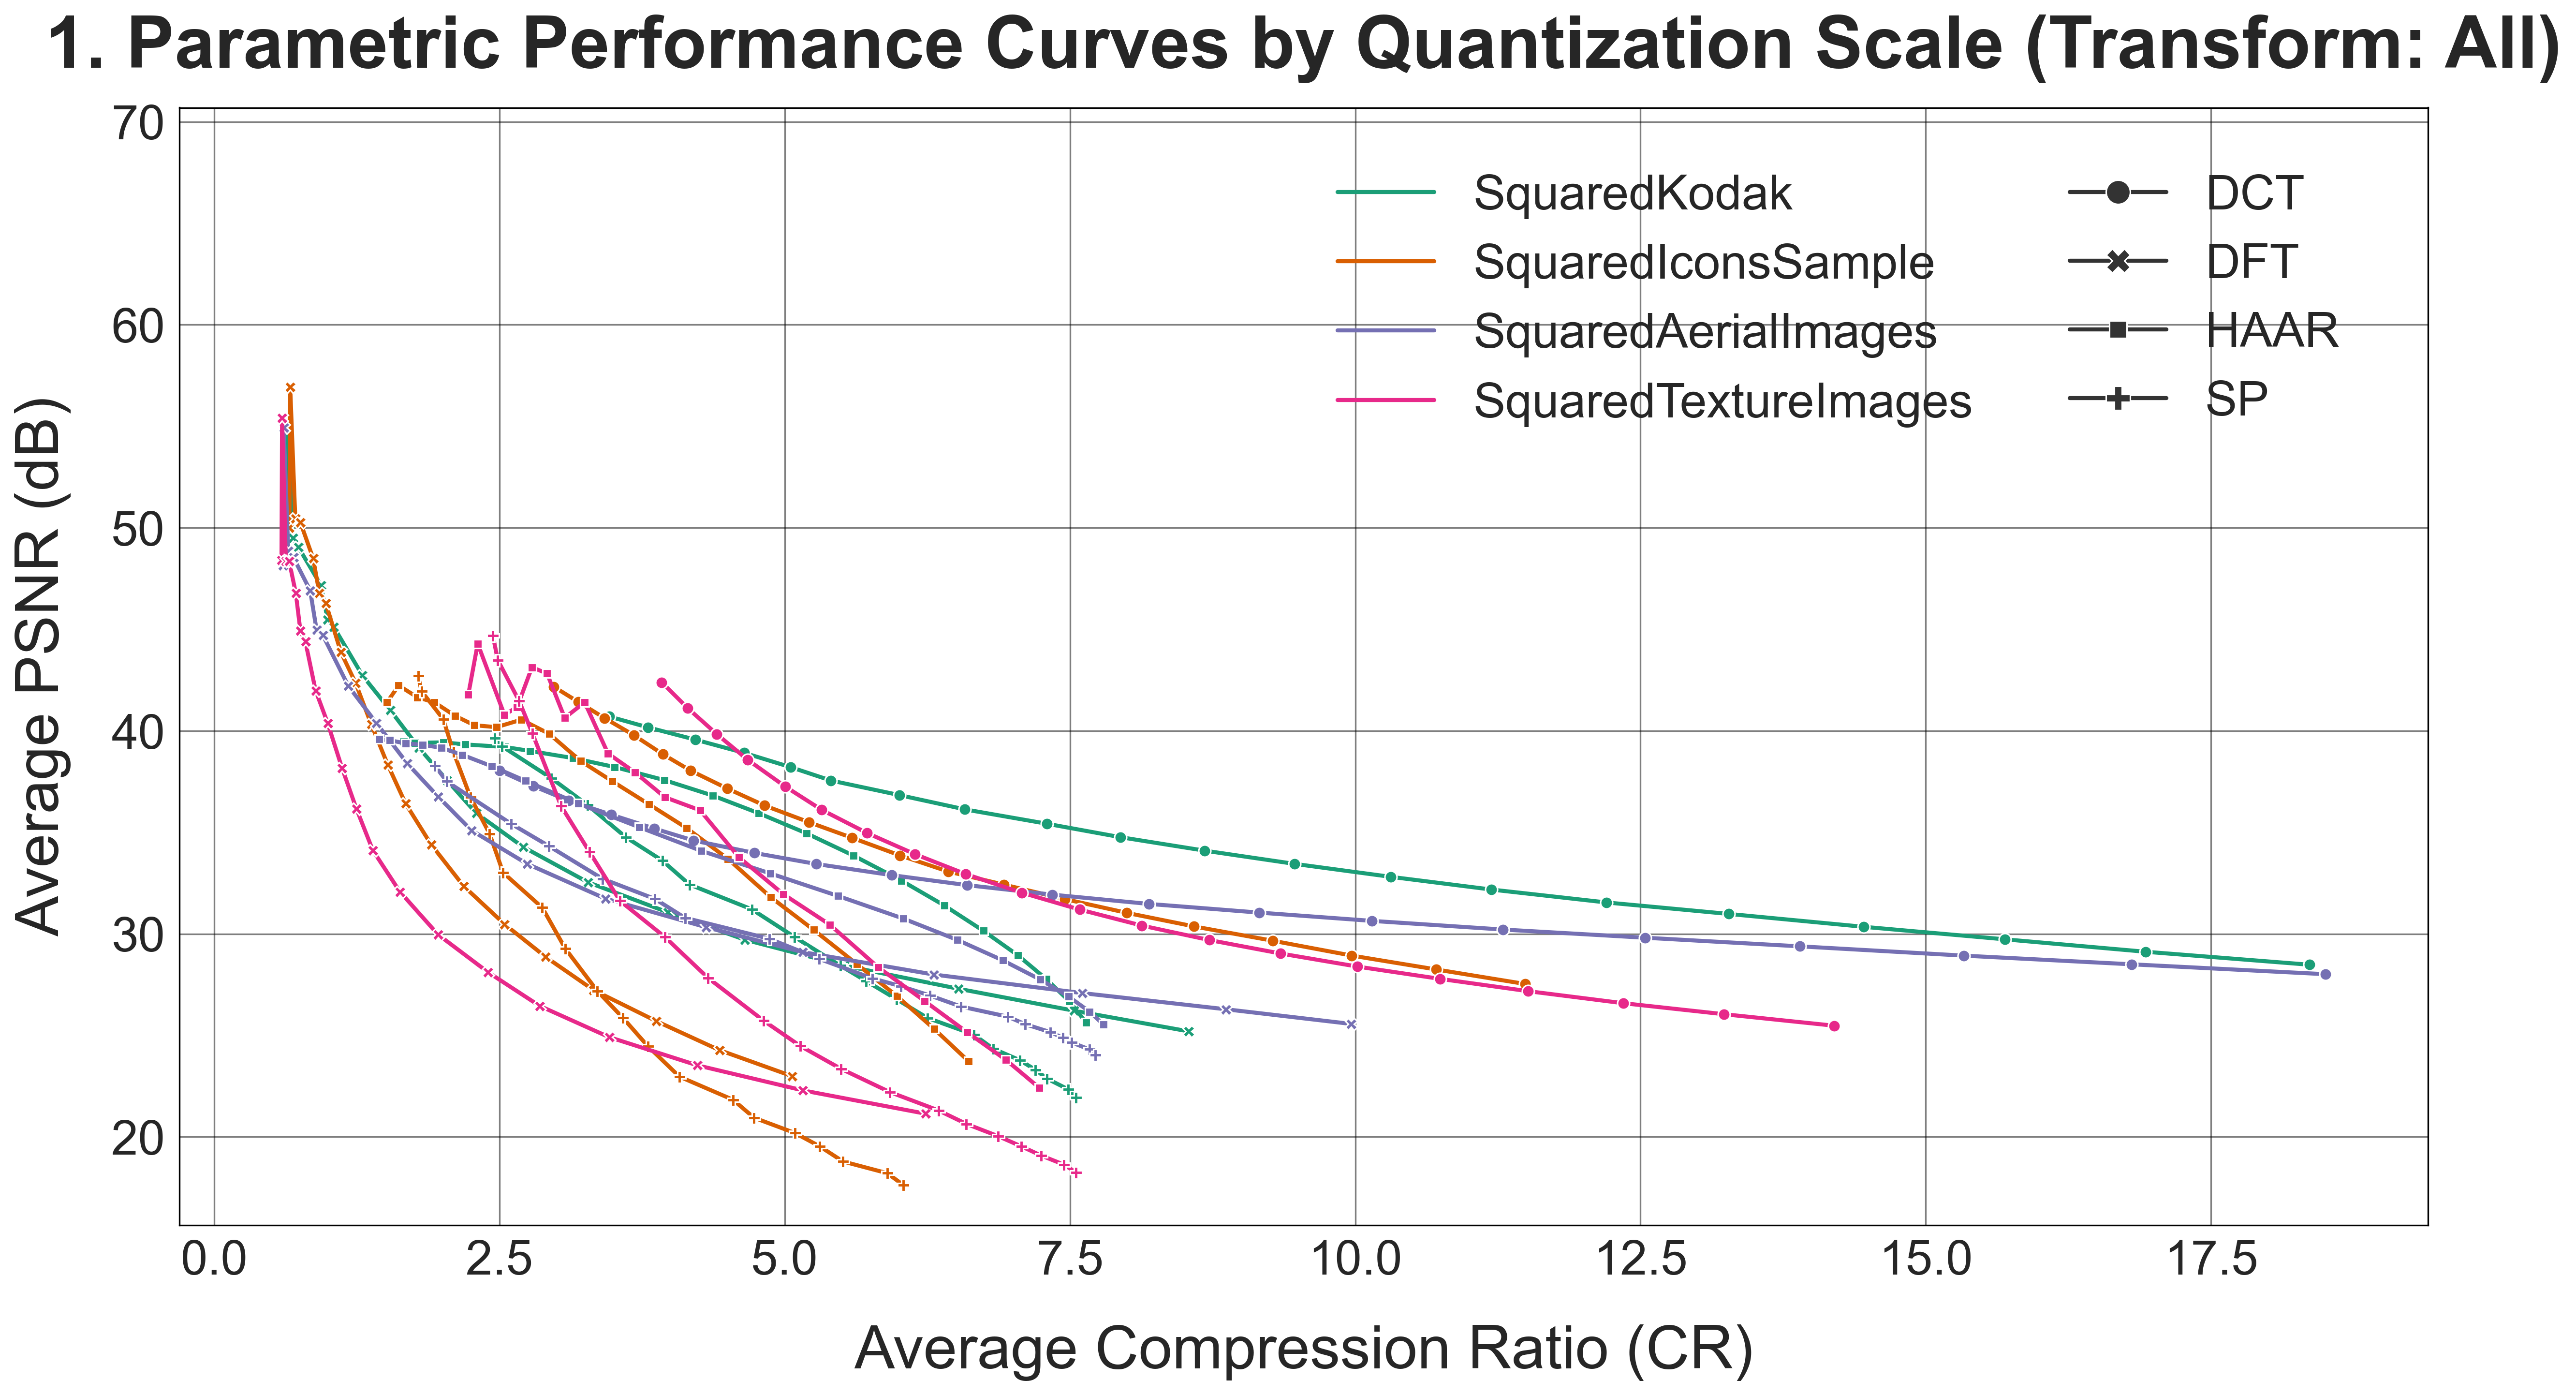
\includegraphics[width=1\linewidth]{results/plots/plot_1_parametric_curve_All.png}
    \caption{Compressed image similarity based on compression ratio by transform and dataset.}
    \label{fig:parametricAll}
\end{figure}

Firstly, as shown in fig. \ref{fig:parametricAll}, all transforms' had their quality of compressed images compared against compression ratio. Quality of compressed images, measured by the similarity between compressed and original image, or PSNR (db), is much higher for DCT, colored in blue, than all other transforms at all compression levels, with DCT additionally reaching higher compression levels than any other transform. Fig. \ref{fig:effectEntropyCoding} explores compression ratio by transform, with each box per transform representing compression ratio data with or without entropy coding used. For DCT and DFT, entropy coding generally increases compression ratio, with significant increases to the highest compression ratios achieved. On the other hand, Haar and SP see a flat decrease in compression ratio when entropy coding is used.

\begin{figure}
    \centering
    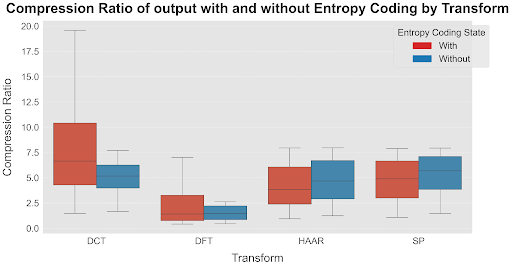
\includegraphics[width=1\linewidth]{results/plots/huffmancomparison.png}
    \caption{Effect of entropy encoding on compression ratio for all transforms}
    \label{fig:effectEntropyCoding}
\end{figure}



\subsection{DWT Results}
\label{resultssec:DWT}
% Content for DWT Results subsection
% This file is included in the main conference paper via % Content for DWT Results subsection
% This file is included in the main conference paper via % Content for DWT Results subsection
% This file is included in the main conference paper via \input{DWTResults}

\begin{figure}[ht]
  \centering
  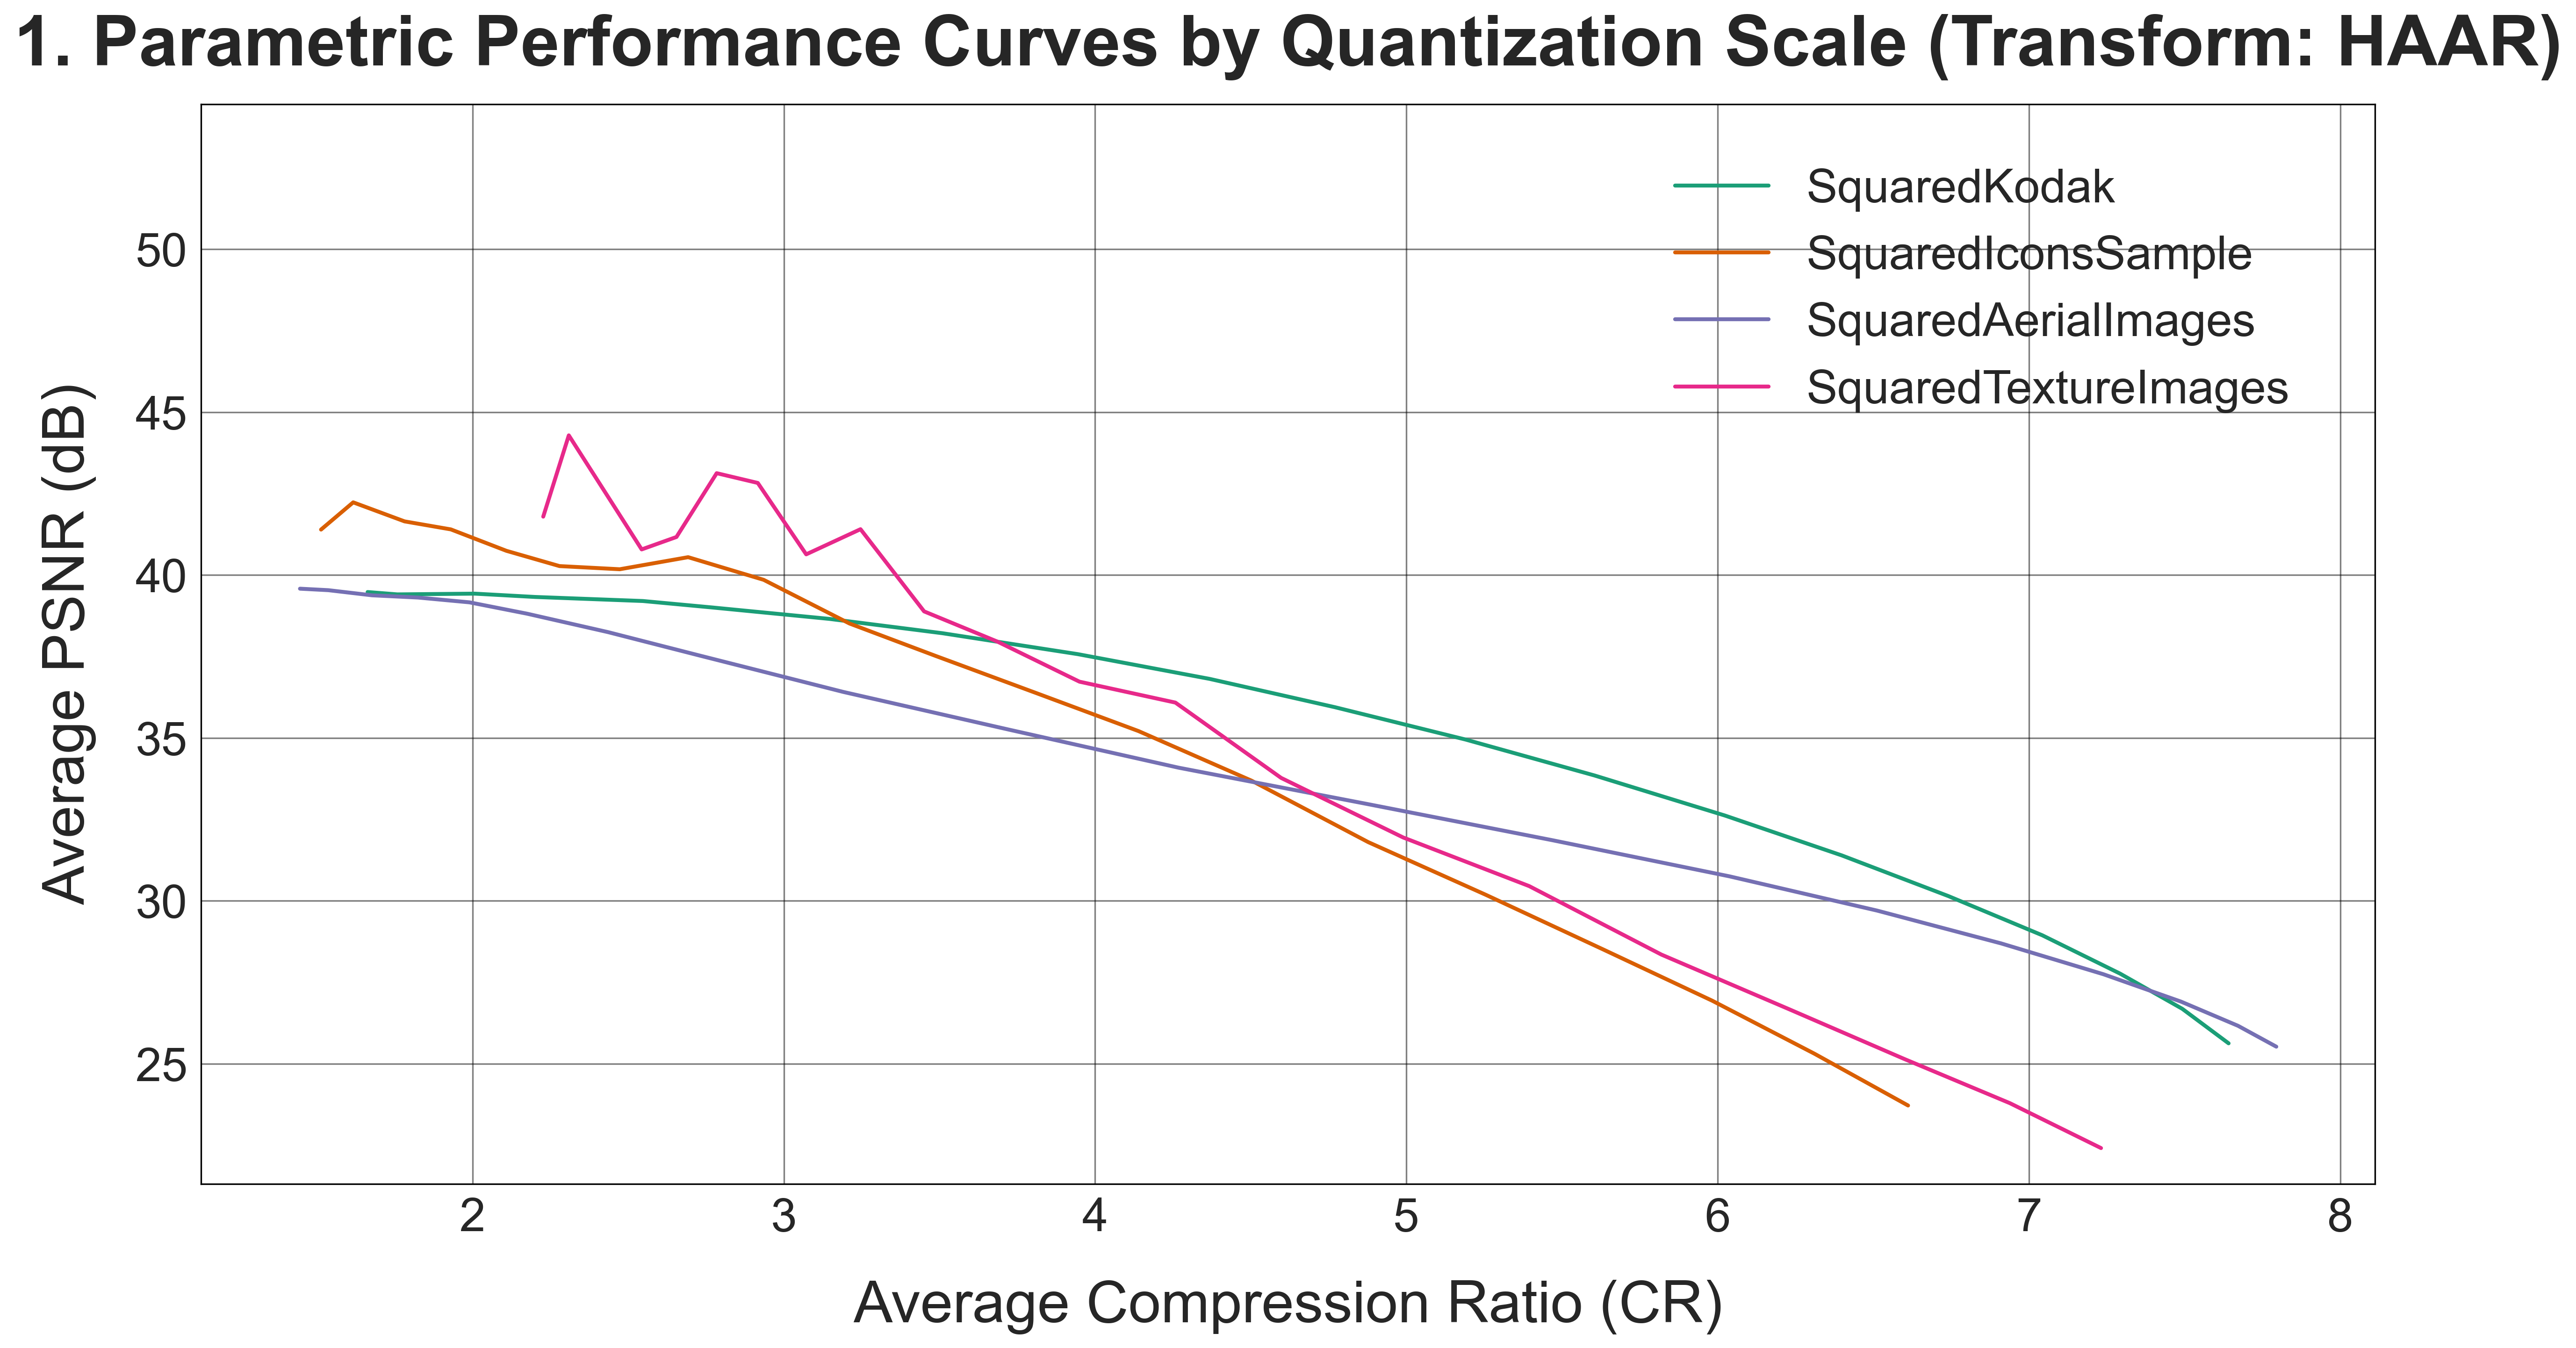
\includegraphics[width=0.48\textwidth]{results/plots/plot_1_parametric_curve_HAAR.png}
  \caption{Performance of the Haar wavelet transform across different datasets}
  \label{fig:dwt_results}
\end{figure}

The results demonstrate that the Discrete Wavelet Transform (DWT) using the Haar wavelet basis exhibits varying performance across different image datasets. Notably, the method performed worse on the Texture Images and Icons Images datasets as quantization became more aggressive compared to other image types as can be see in Figure~\ref{fig:dwt_results}.

\begin{figure}[ht]
  \centering
  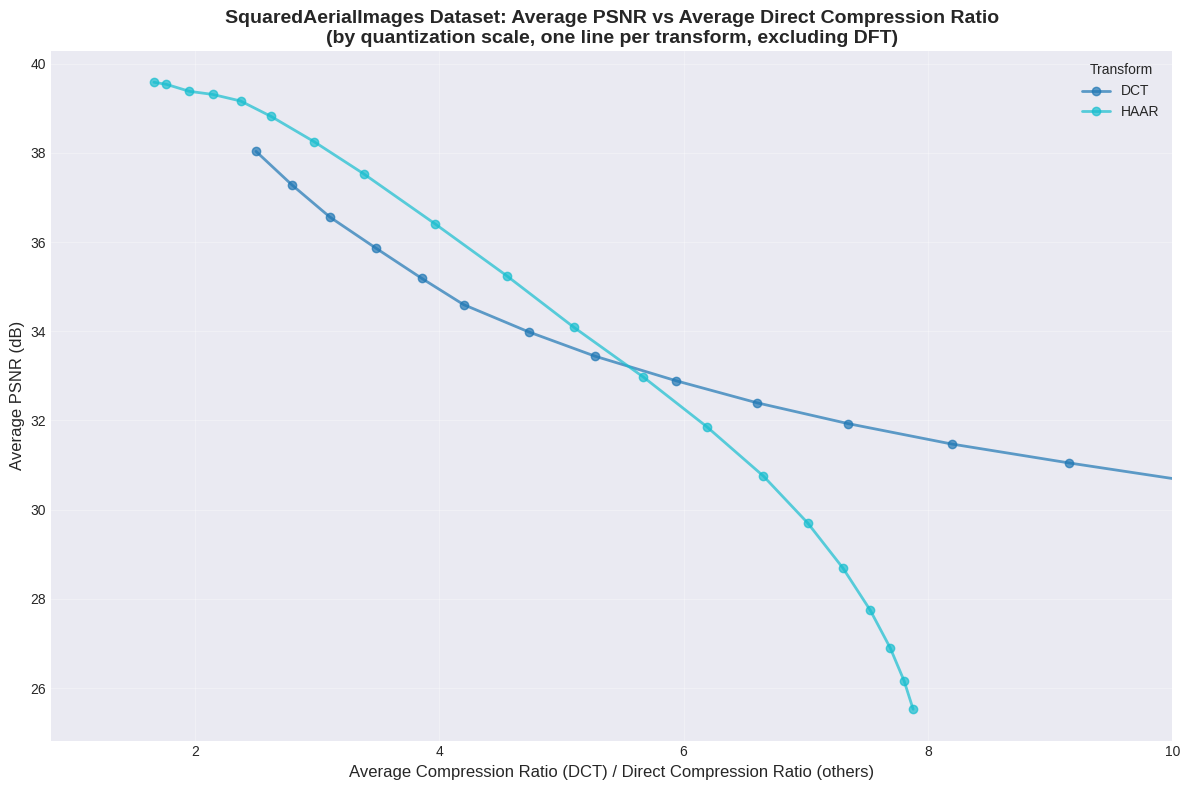
\includegraphics[width=0.48\textwidth]{results/plots/parametric_aerial.png}
  \caption{Performance comparison of Haar and DCT on aerial images.}
  \label{fig:dwt_aerial}
\end{figure}

Figure~\ref{fig:dwt_aerial} shows that the Haar wavelet transform performs slightly better than DCT on aerial images at smaller compression ratios.

\begin{figure}[ht]
  \centering
  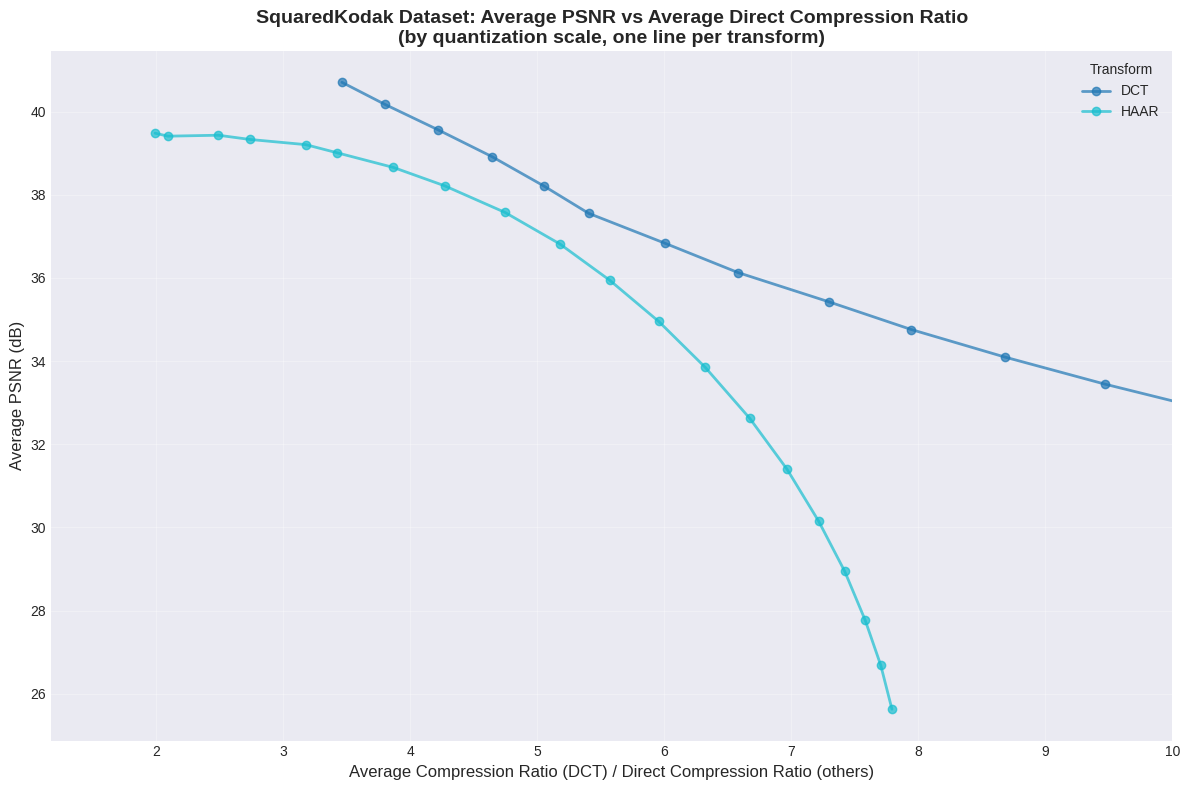
\includegraphics[width=0.48\textwidth]{results/plots/parametric_kodak.png}
  \caption{Performance comparison of Haar and DCT on Kodak images.}
  \label{fig:dwt_kodak}
\end{figure}

In contrast, Figure~\ref{fig:dwt_kodak} demonstrates that Haar performs worse than DCT on Kodak images across all compression ratio scenarios.


\begin{figure}[ht]
  \centering
  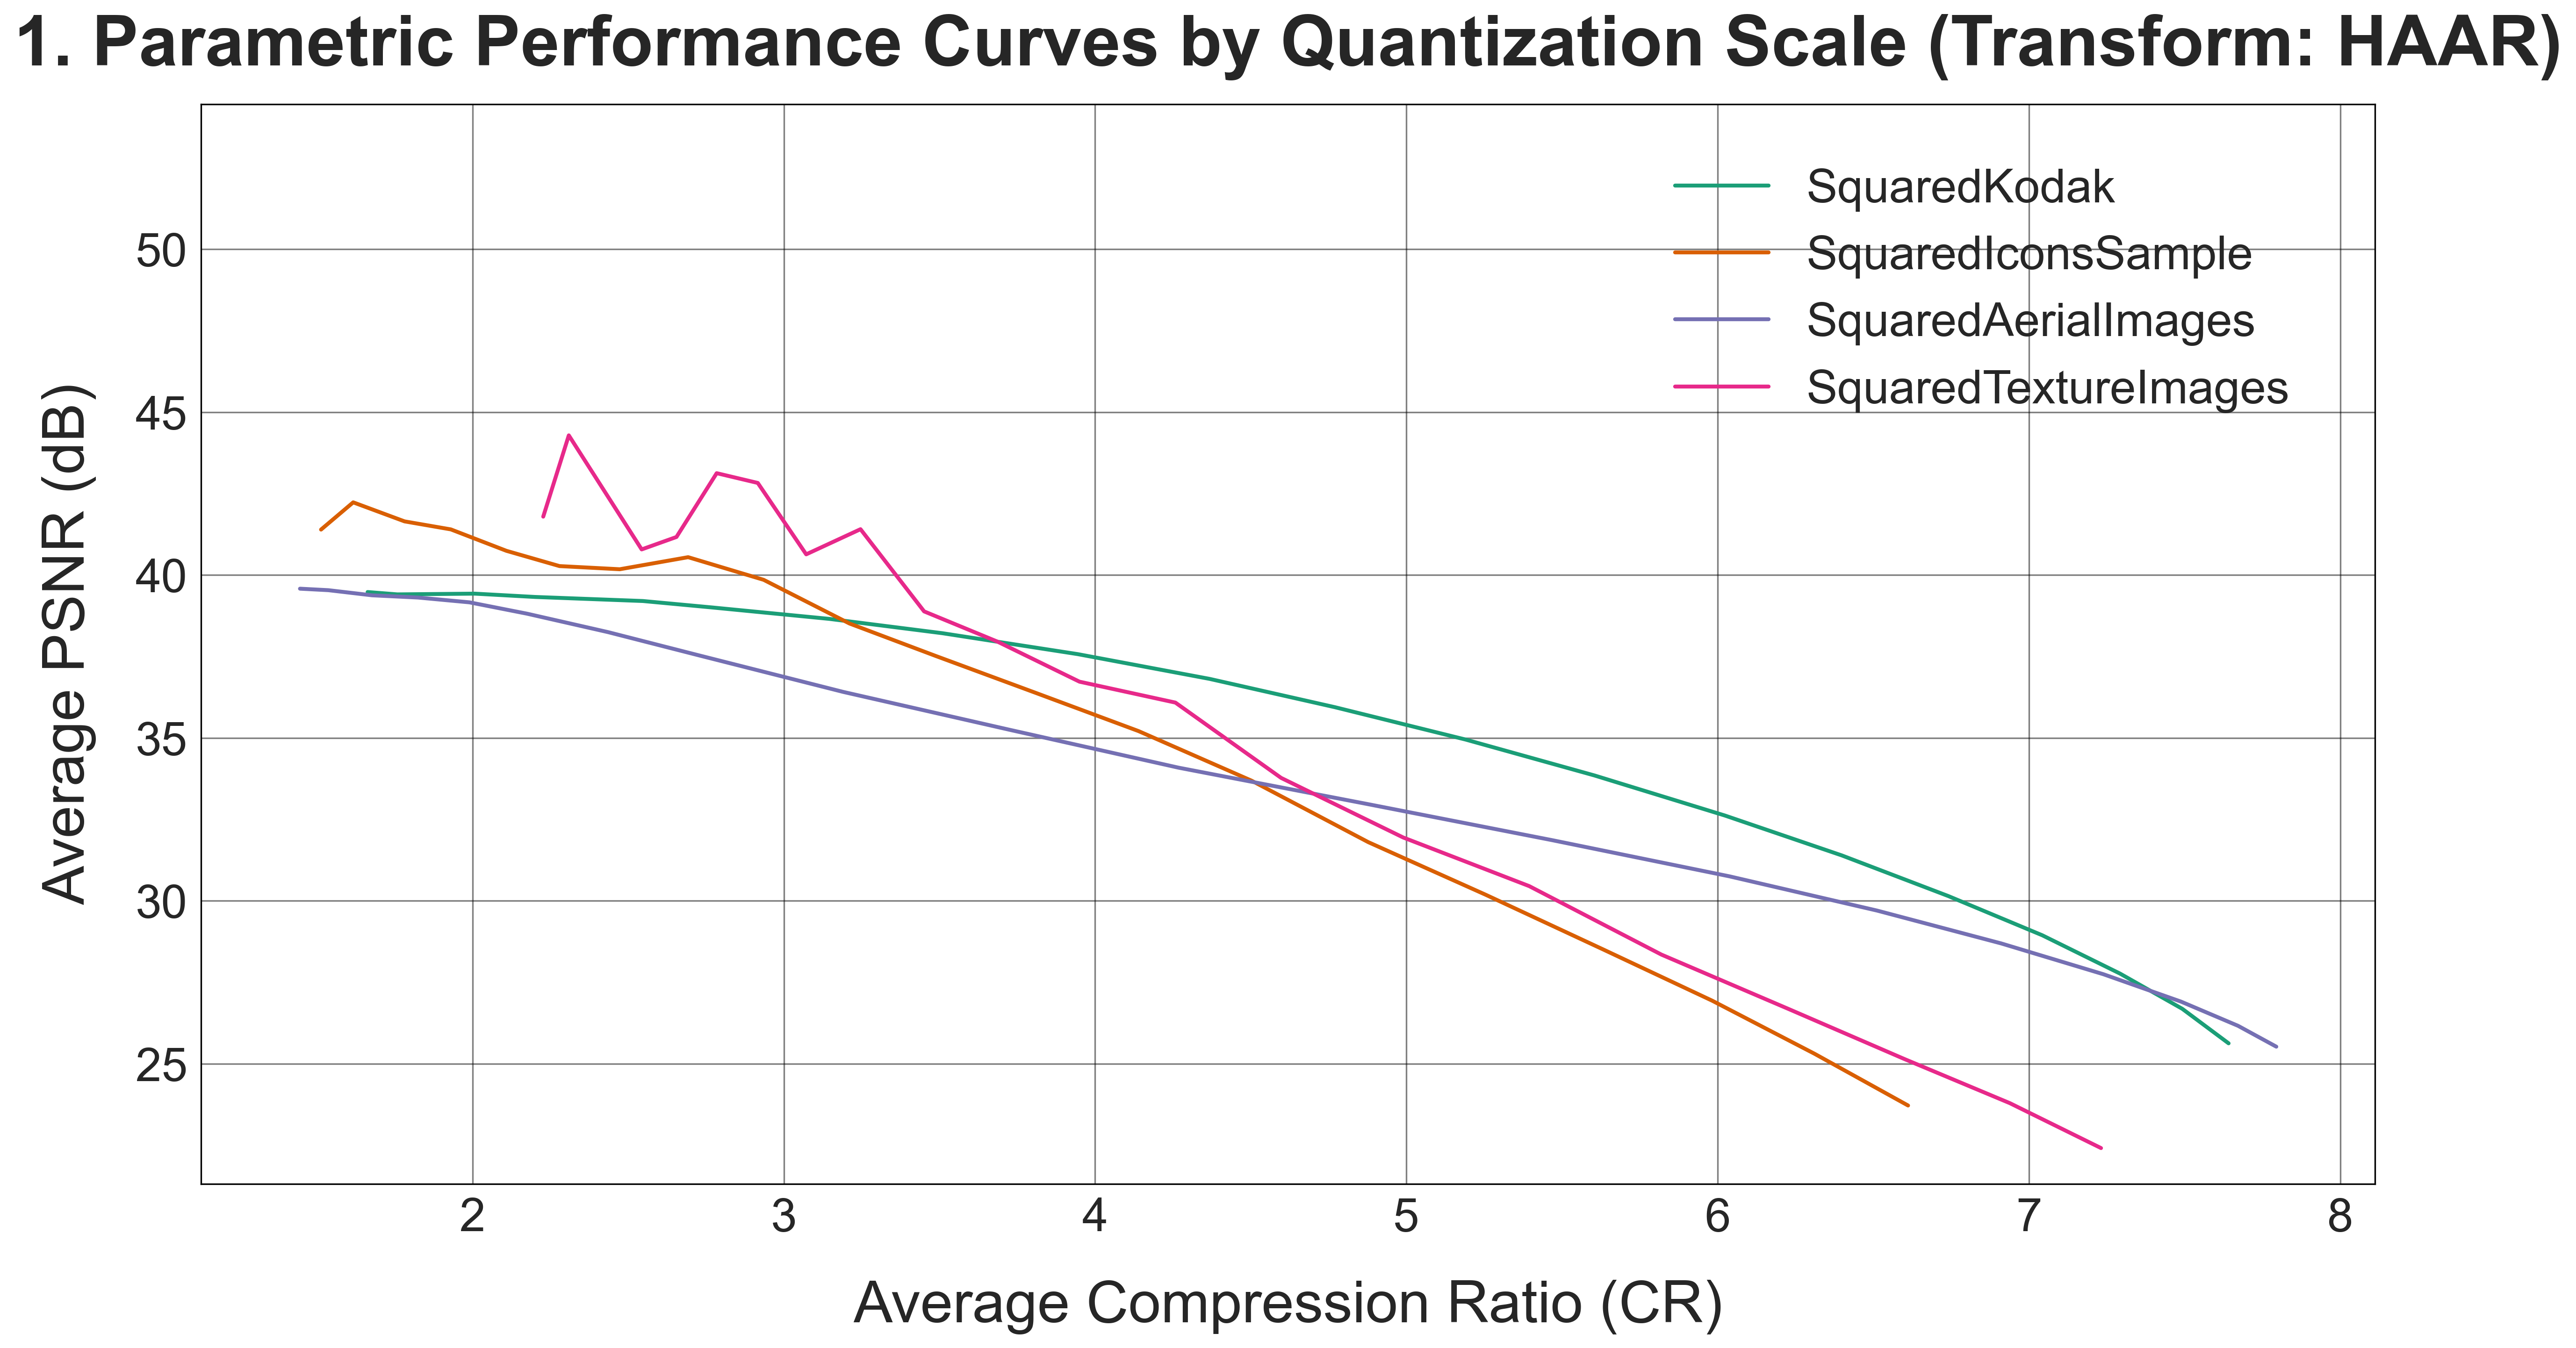
\includegraphics[width=0.48\textwidth]{results/plots/plot_1_parametric_curve_HAAR.png}
  \caption{Performance of the Haar wavelet transform across different datasets}
  \label{fig:dwt_results}
\end{figure}

The results demonstrate that the Discrete Wavelet Transform (DWT) using the Haar wavelet basis exhibits varying performance across different image datasets. Notably, the method performed worse on the Texture Images and Icons Images datasets as quantization became more aggressive compared to other image types as can be see in Figure~\ref{fig:dwt_results}.

\begin{figure}[ht]
  \centering
  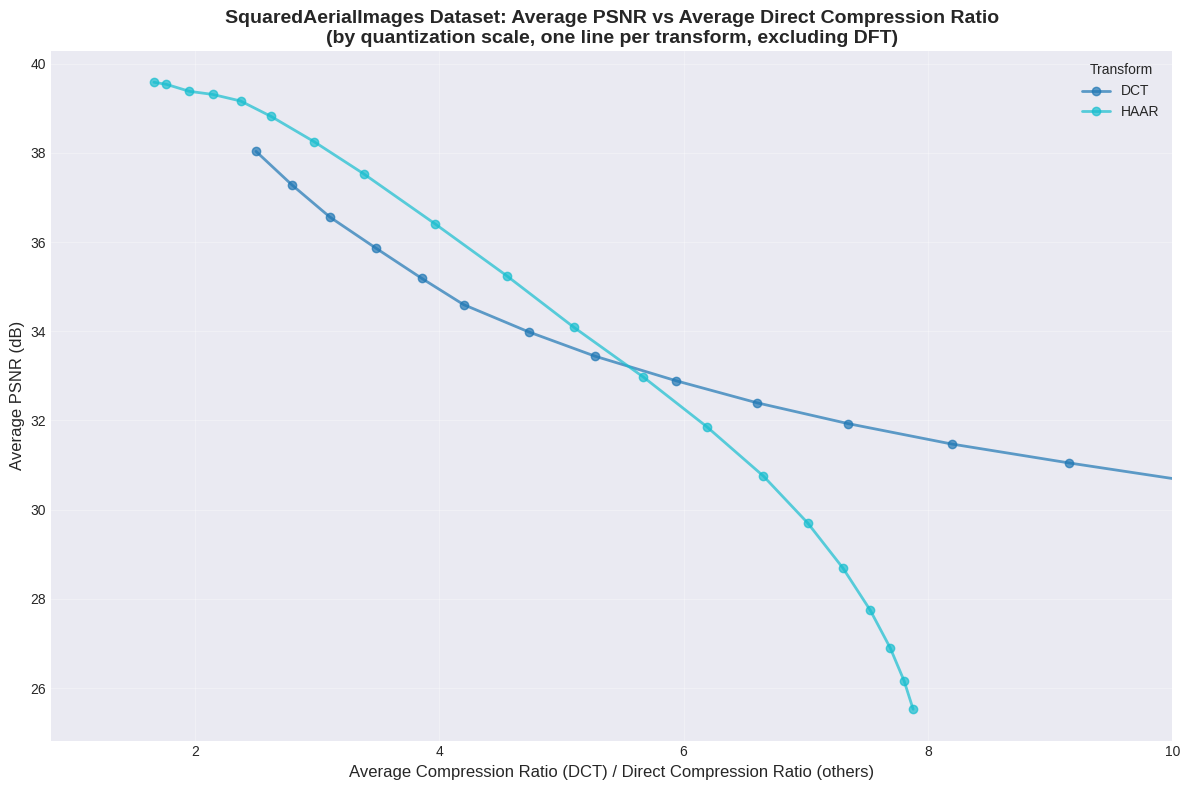
\includegraphics[width=0.48\textwidth]{results/plots/parametric_aerial.png}
  \caption{Performance comparison of Haar and DCT on aerial images.}
  \label{fig:dwt_aerial}
\end{figure}

Figure~\ref{fig:dwt_aerial} shows that the Haar wavelet transform performs slightly better than DCT on aerial images at smaller compression ratios.

\begin{figure}[ht]
  \centering
  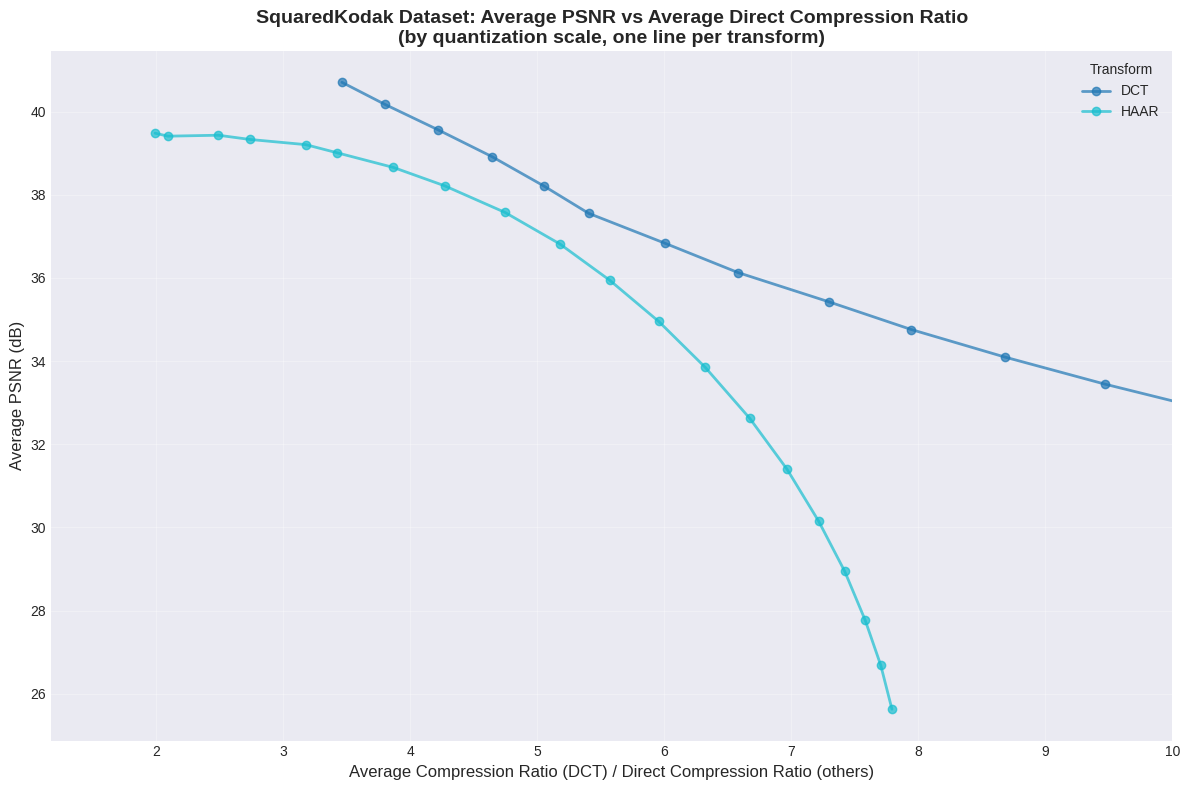
\includegraphics[width=0.48\textwidth]{results/plots/parametric_kodak.png}
  \caption{Performance comparison of Haar and DCT on Kodak images.}
  \label{fig:dwt_kodak}
\end{figure}

In contrast, Figure~\ref{fig:dwt_kodak} demonstrates that Haar performs worse than DCT on Kodak images across all compression ratio scenarios.


\begin{figure}[ht]
  \centering
  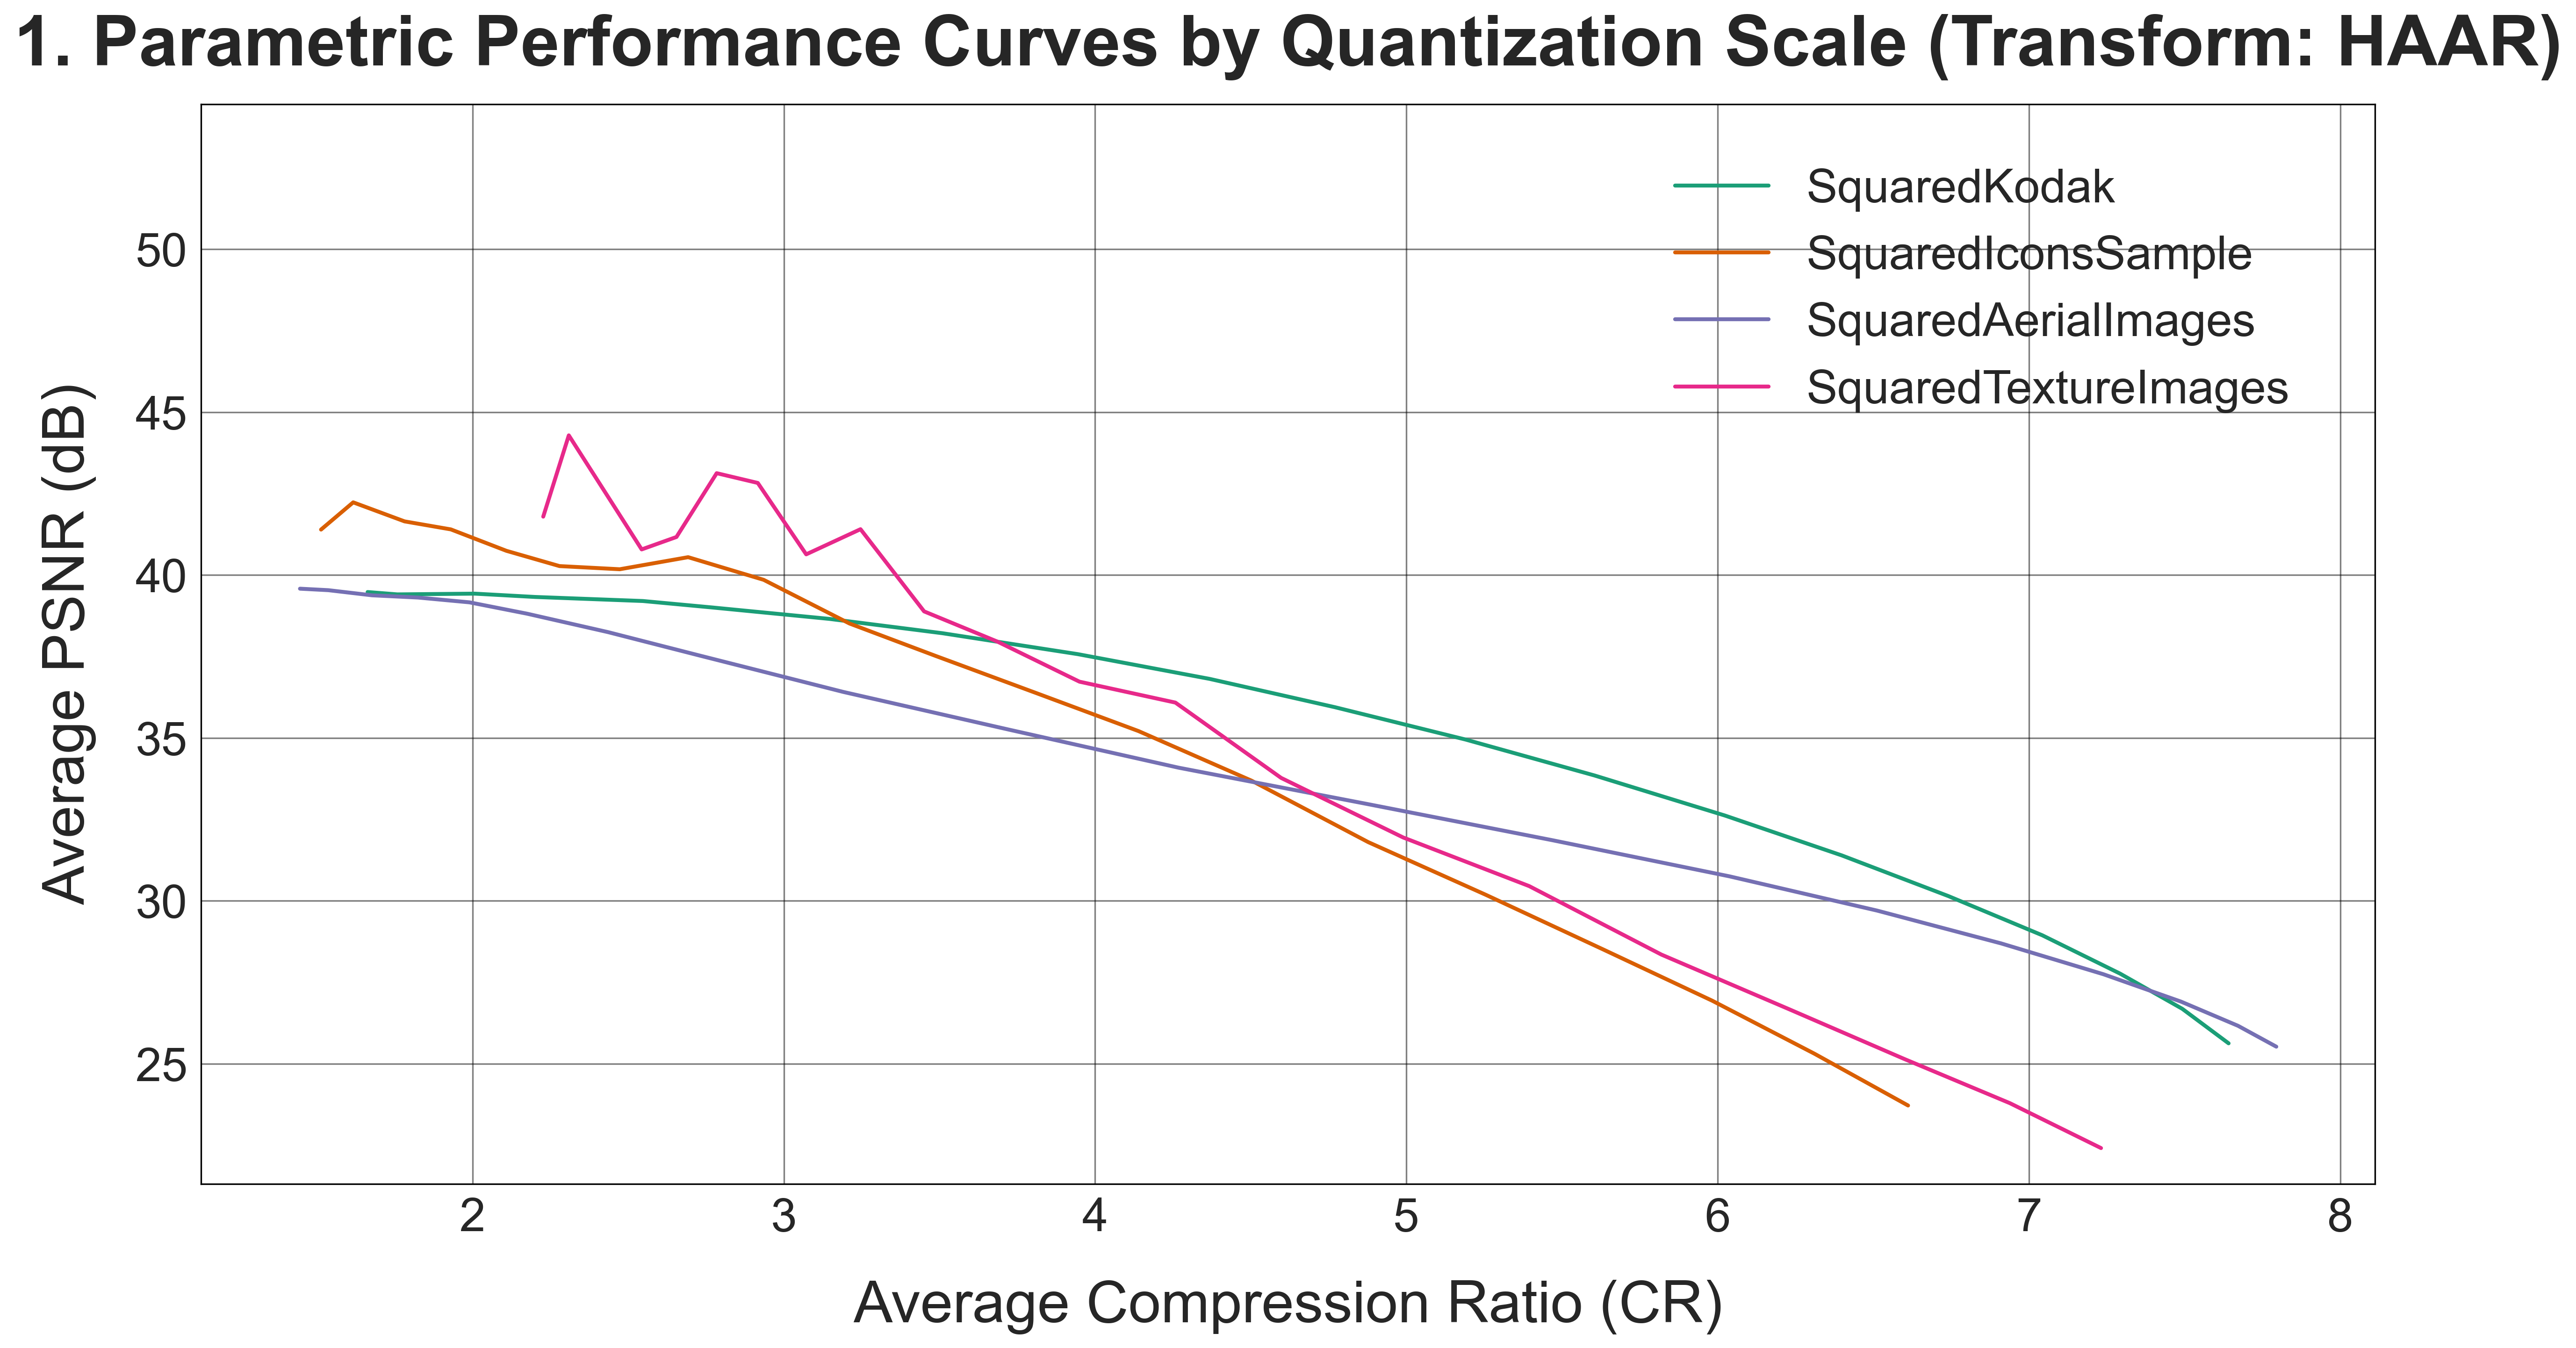
\includegraphics[width=0.48\textwidth]{results/plots/plot_1_parametric_curve_HAAR.png}
  \caption{Performance of the Haar wavelet transform across different datasets}
  \label{fig:dwt_results}
\end{figure}

The results demonstrate that the Discrete Wavelet Transform (DWT) using the Haar wavelet basis exhibits varying performance across different image datasets. Notably, the method performed worse on the Texture Images and Icons Images datasets as quantization became more aggressive compared to other image types as can be see in Figure~\ref{fig:dwt_results}.

\begin{figure}[ht]
  \centering
  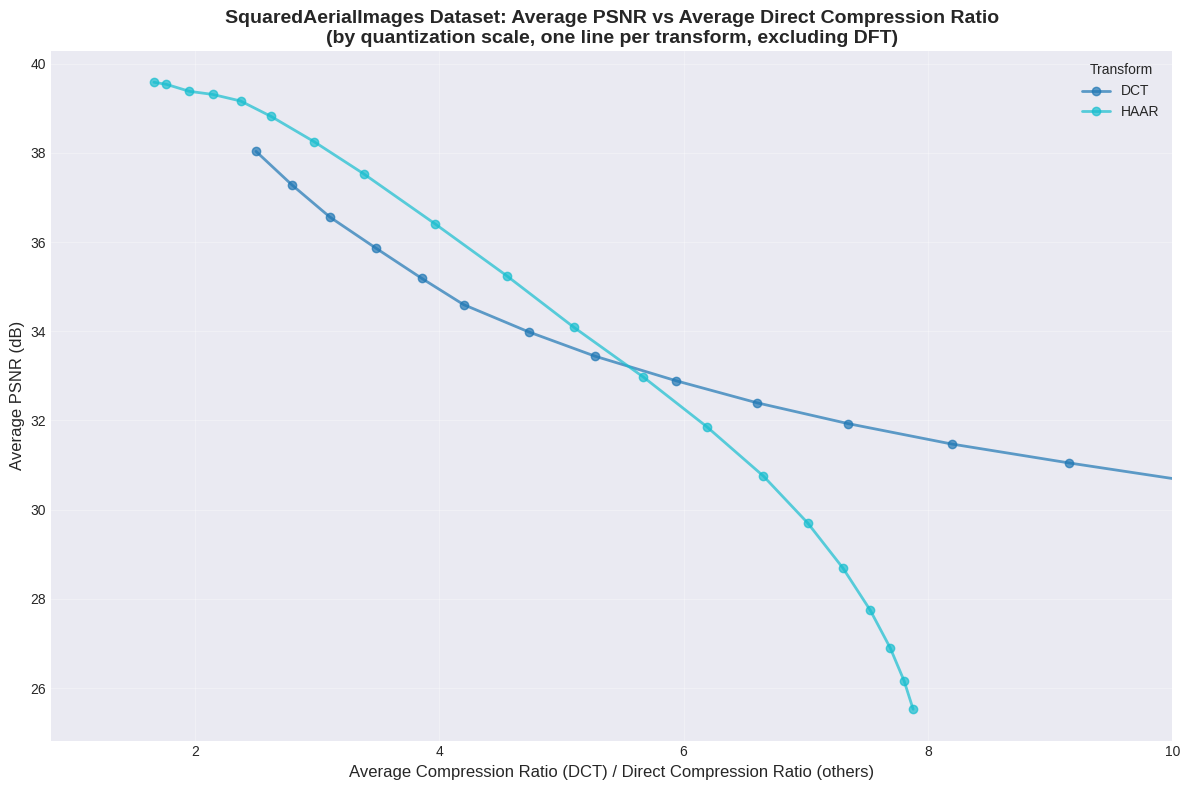
\includegraphics[width=0.48\textwidth]{results/plots/parametric_aerial.png}
  \caption{Performance comparison of Haar and DCT on aerial images.}
  \label{fig:dwt_aerial}
\end{figure}

Figure~\ref{fig:dwt_aerial} shows that the Haar wavelet transform performs slightly better than DCT on aerial images at smaller compression ratios.

\begin{figure}[ht]
  \centering
  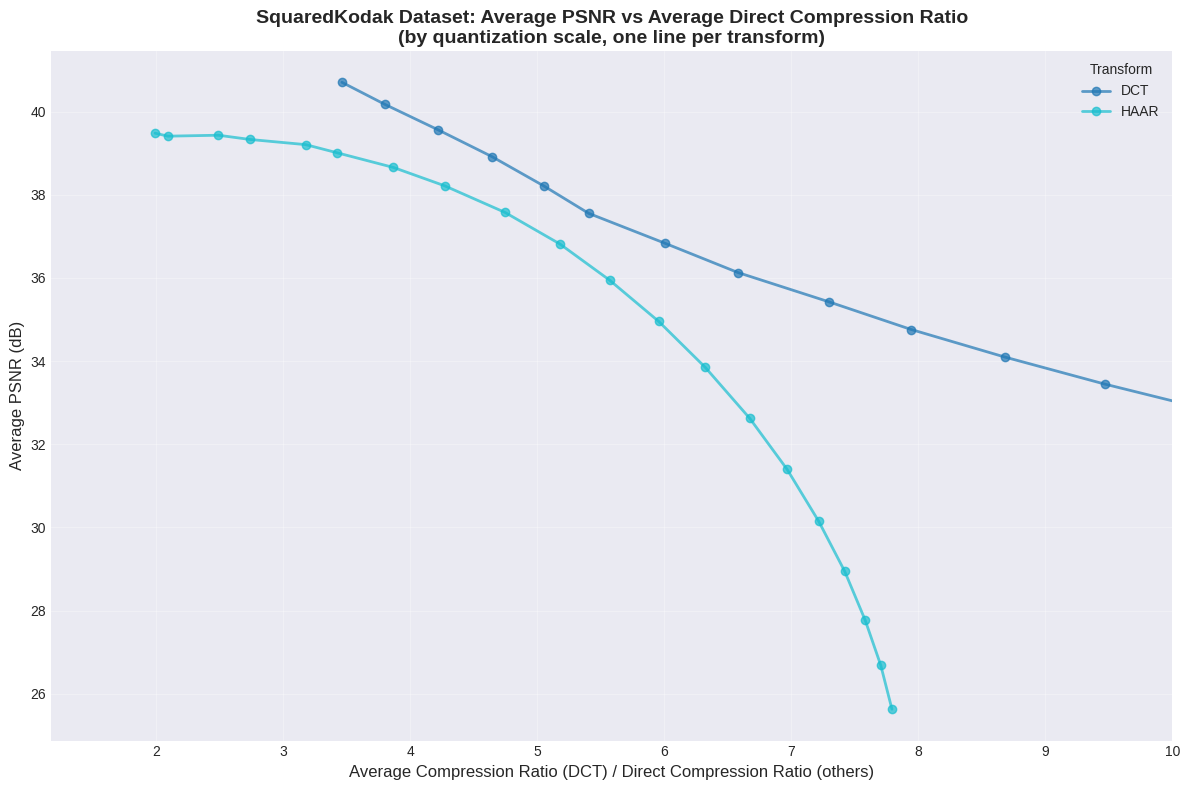
\includegraphics[width=0.48\textwidth]{results/plots/parametric_kodak.png}
  \caption{Performance comparison of Haar and DCT on Kodak images.}
  \label{fig:dwt_kodak}
\end{figure}

In contrast, Figure~\ref{fig:dwt_kodak} demonstrates that Haar performs worse than DCT on Kodak images across all compression ratio scenarios.


\subsection{DCT Results}
\label{resultssec:DCT}
% Content for DCT Results subsection
% This file is included in the main conference paper via % Content for DCT Results subsection
% This file is included in the main conference paper via % Content for DCT Results subsection
% This file is included in the main conference paper via \input{DCTResults}

We claimed in \ref{methodsec:fourier} that DCT is superior to DFT for image compression. To see this clearly, Fig. \ref{fig:dctvsdft} shows how DCT achieves much higher compression ratios at equivalent PSNR values across all datasets. For example, at a PSNR of 30 dB, the DFT achieves CR$\approx5$ across all datasets, while DCT has CR$\approx10$, even closer to 15 for Aerial Images. 

\begin{figure}
    \centering
    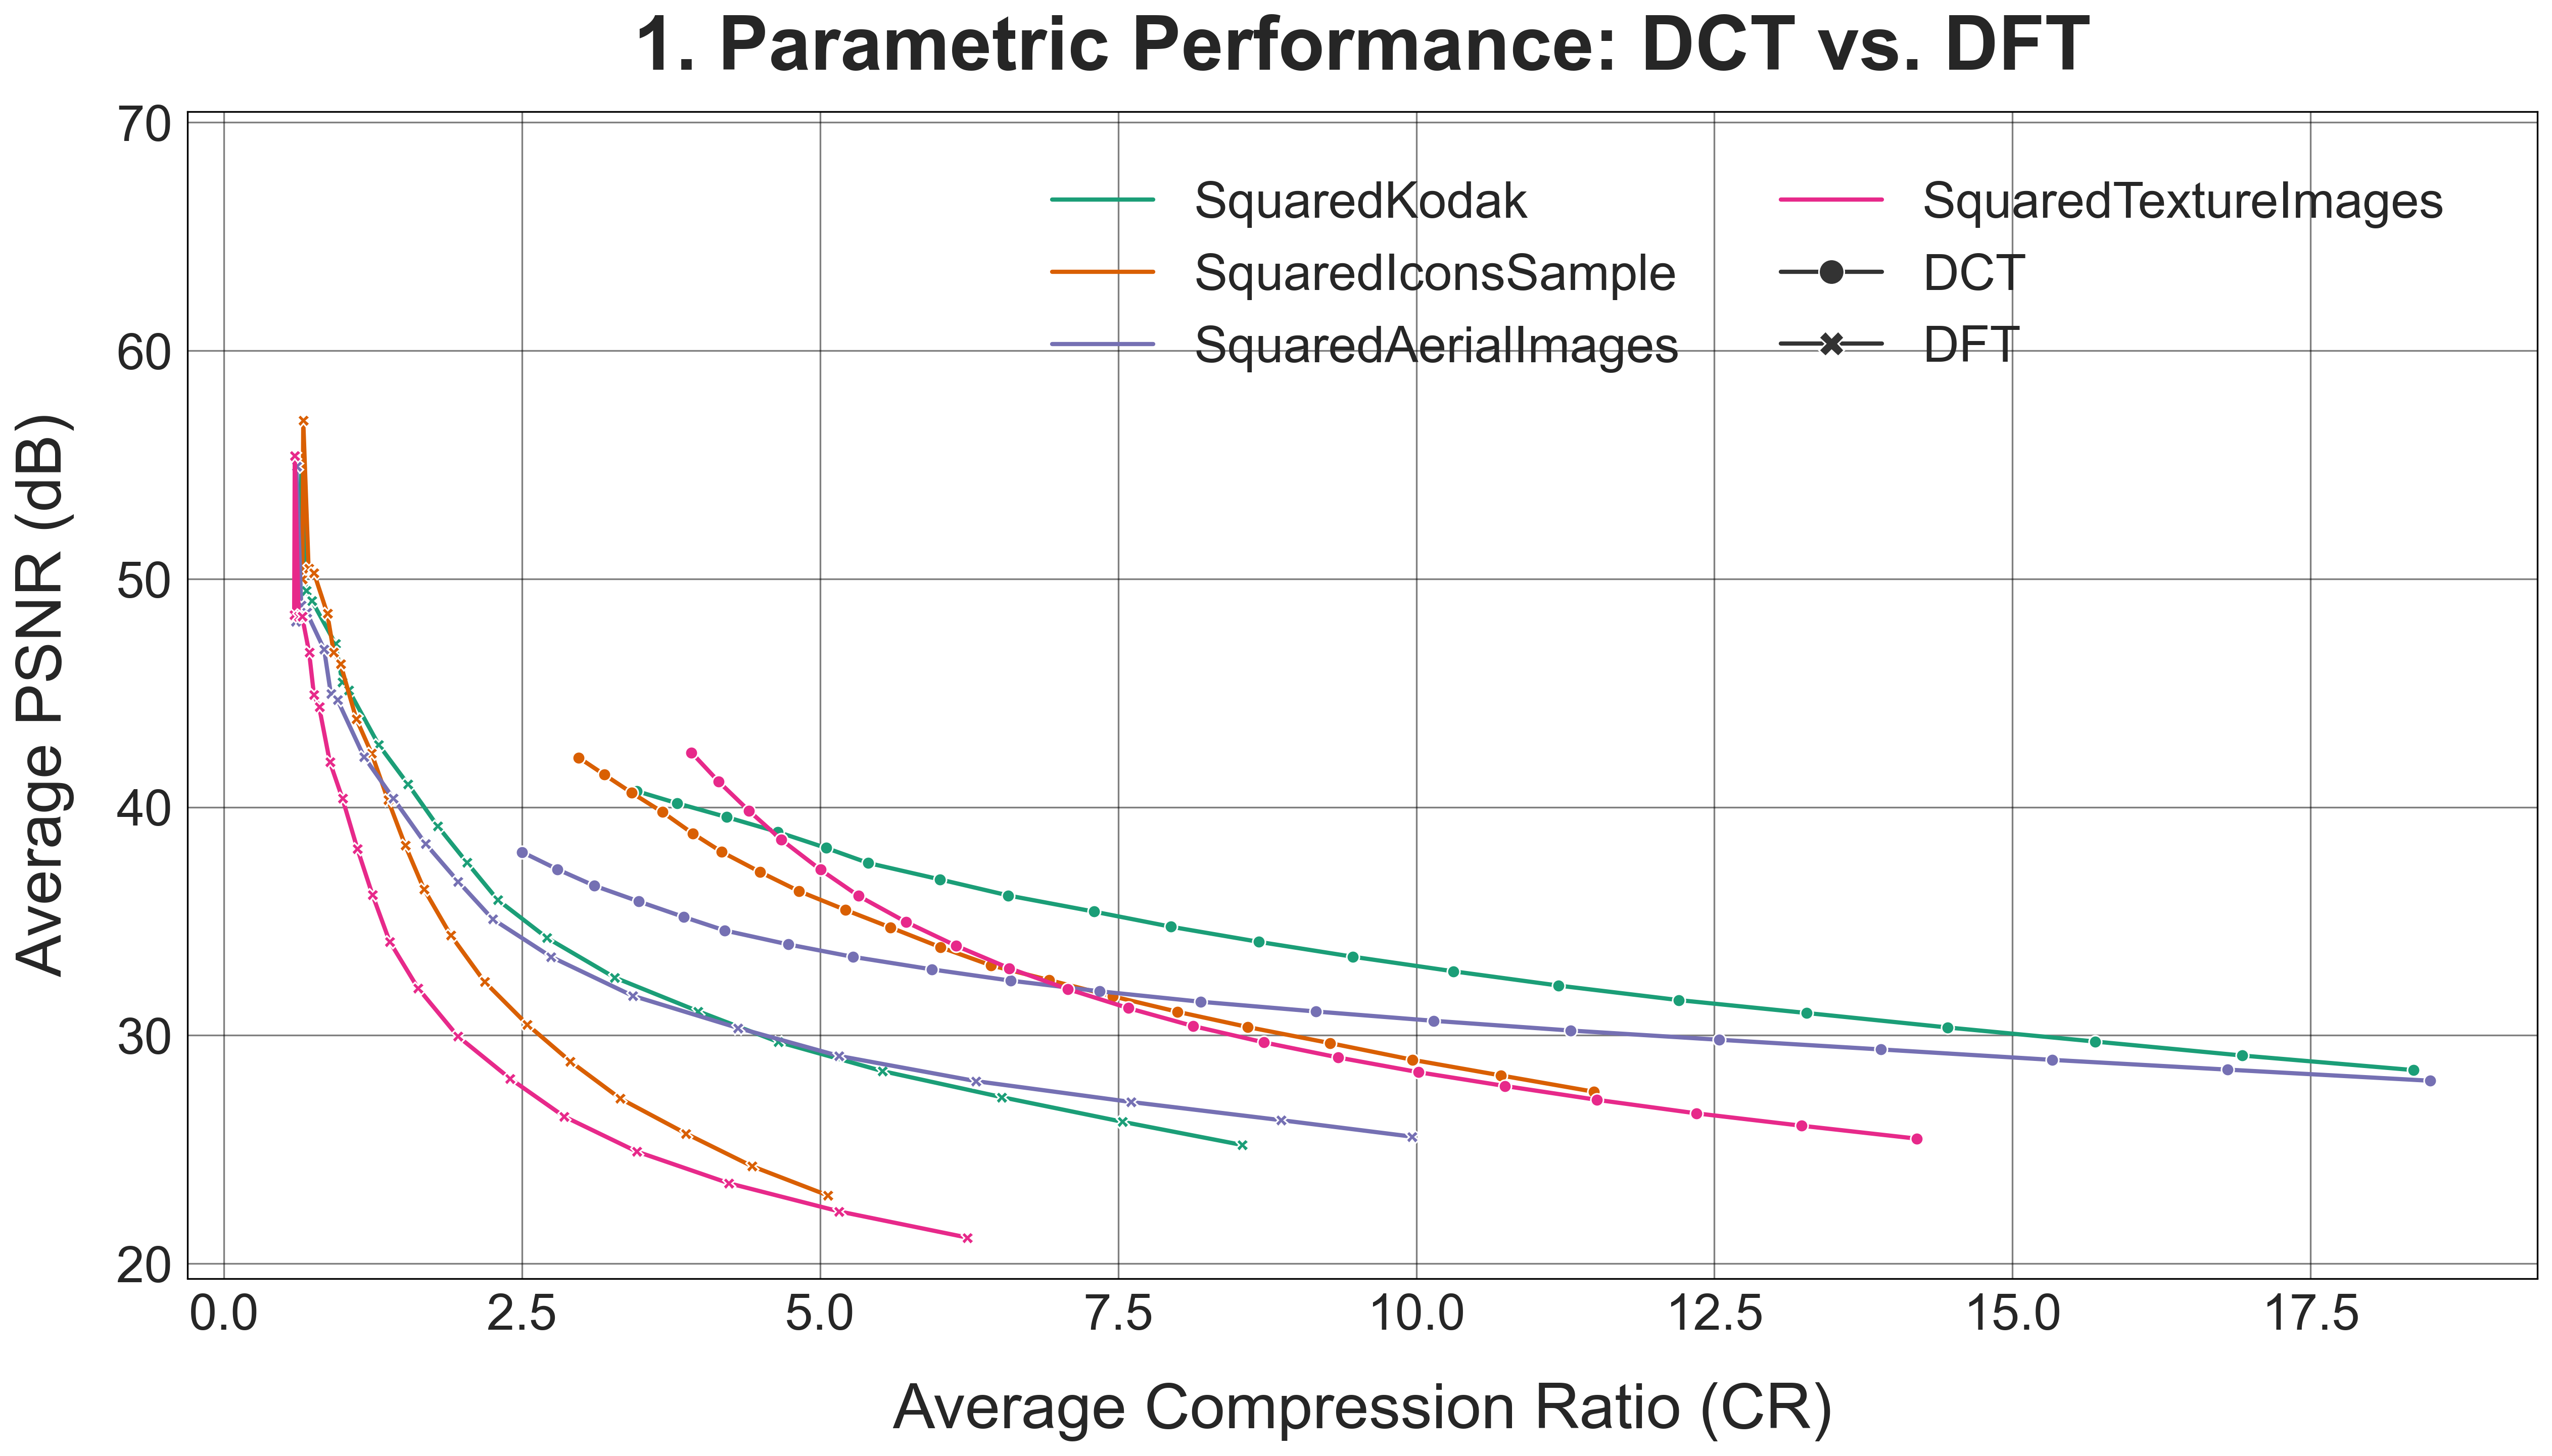
\includegraphics[width=1\linewidth]{results/plots/plot_5_parametric_DCT_vs_DFT.png}
    \caption{Different levels of quantization on sample image with compression ratio.}
    \label{fig:dctvsdft}
\end{figure}

Notably, in \ref{resultssec:col} it appears that the DCT outperforms all transform algorithms, not just the DFT. This comparison is slightly unfair since an additional step RLE was added to the entropy coding for DCT as described in \ref{methodsec:entropy}. Fig. \ref{fig:dctcrvsdcr} shows how the compression ratios change without RLE present for a more fair comparison.

\begin{figure}
    \centering
    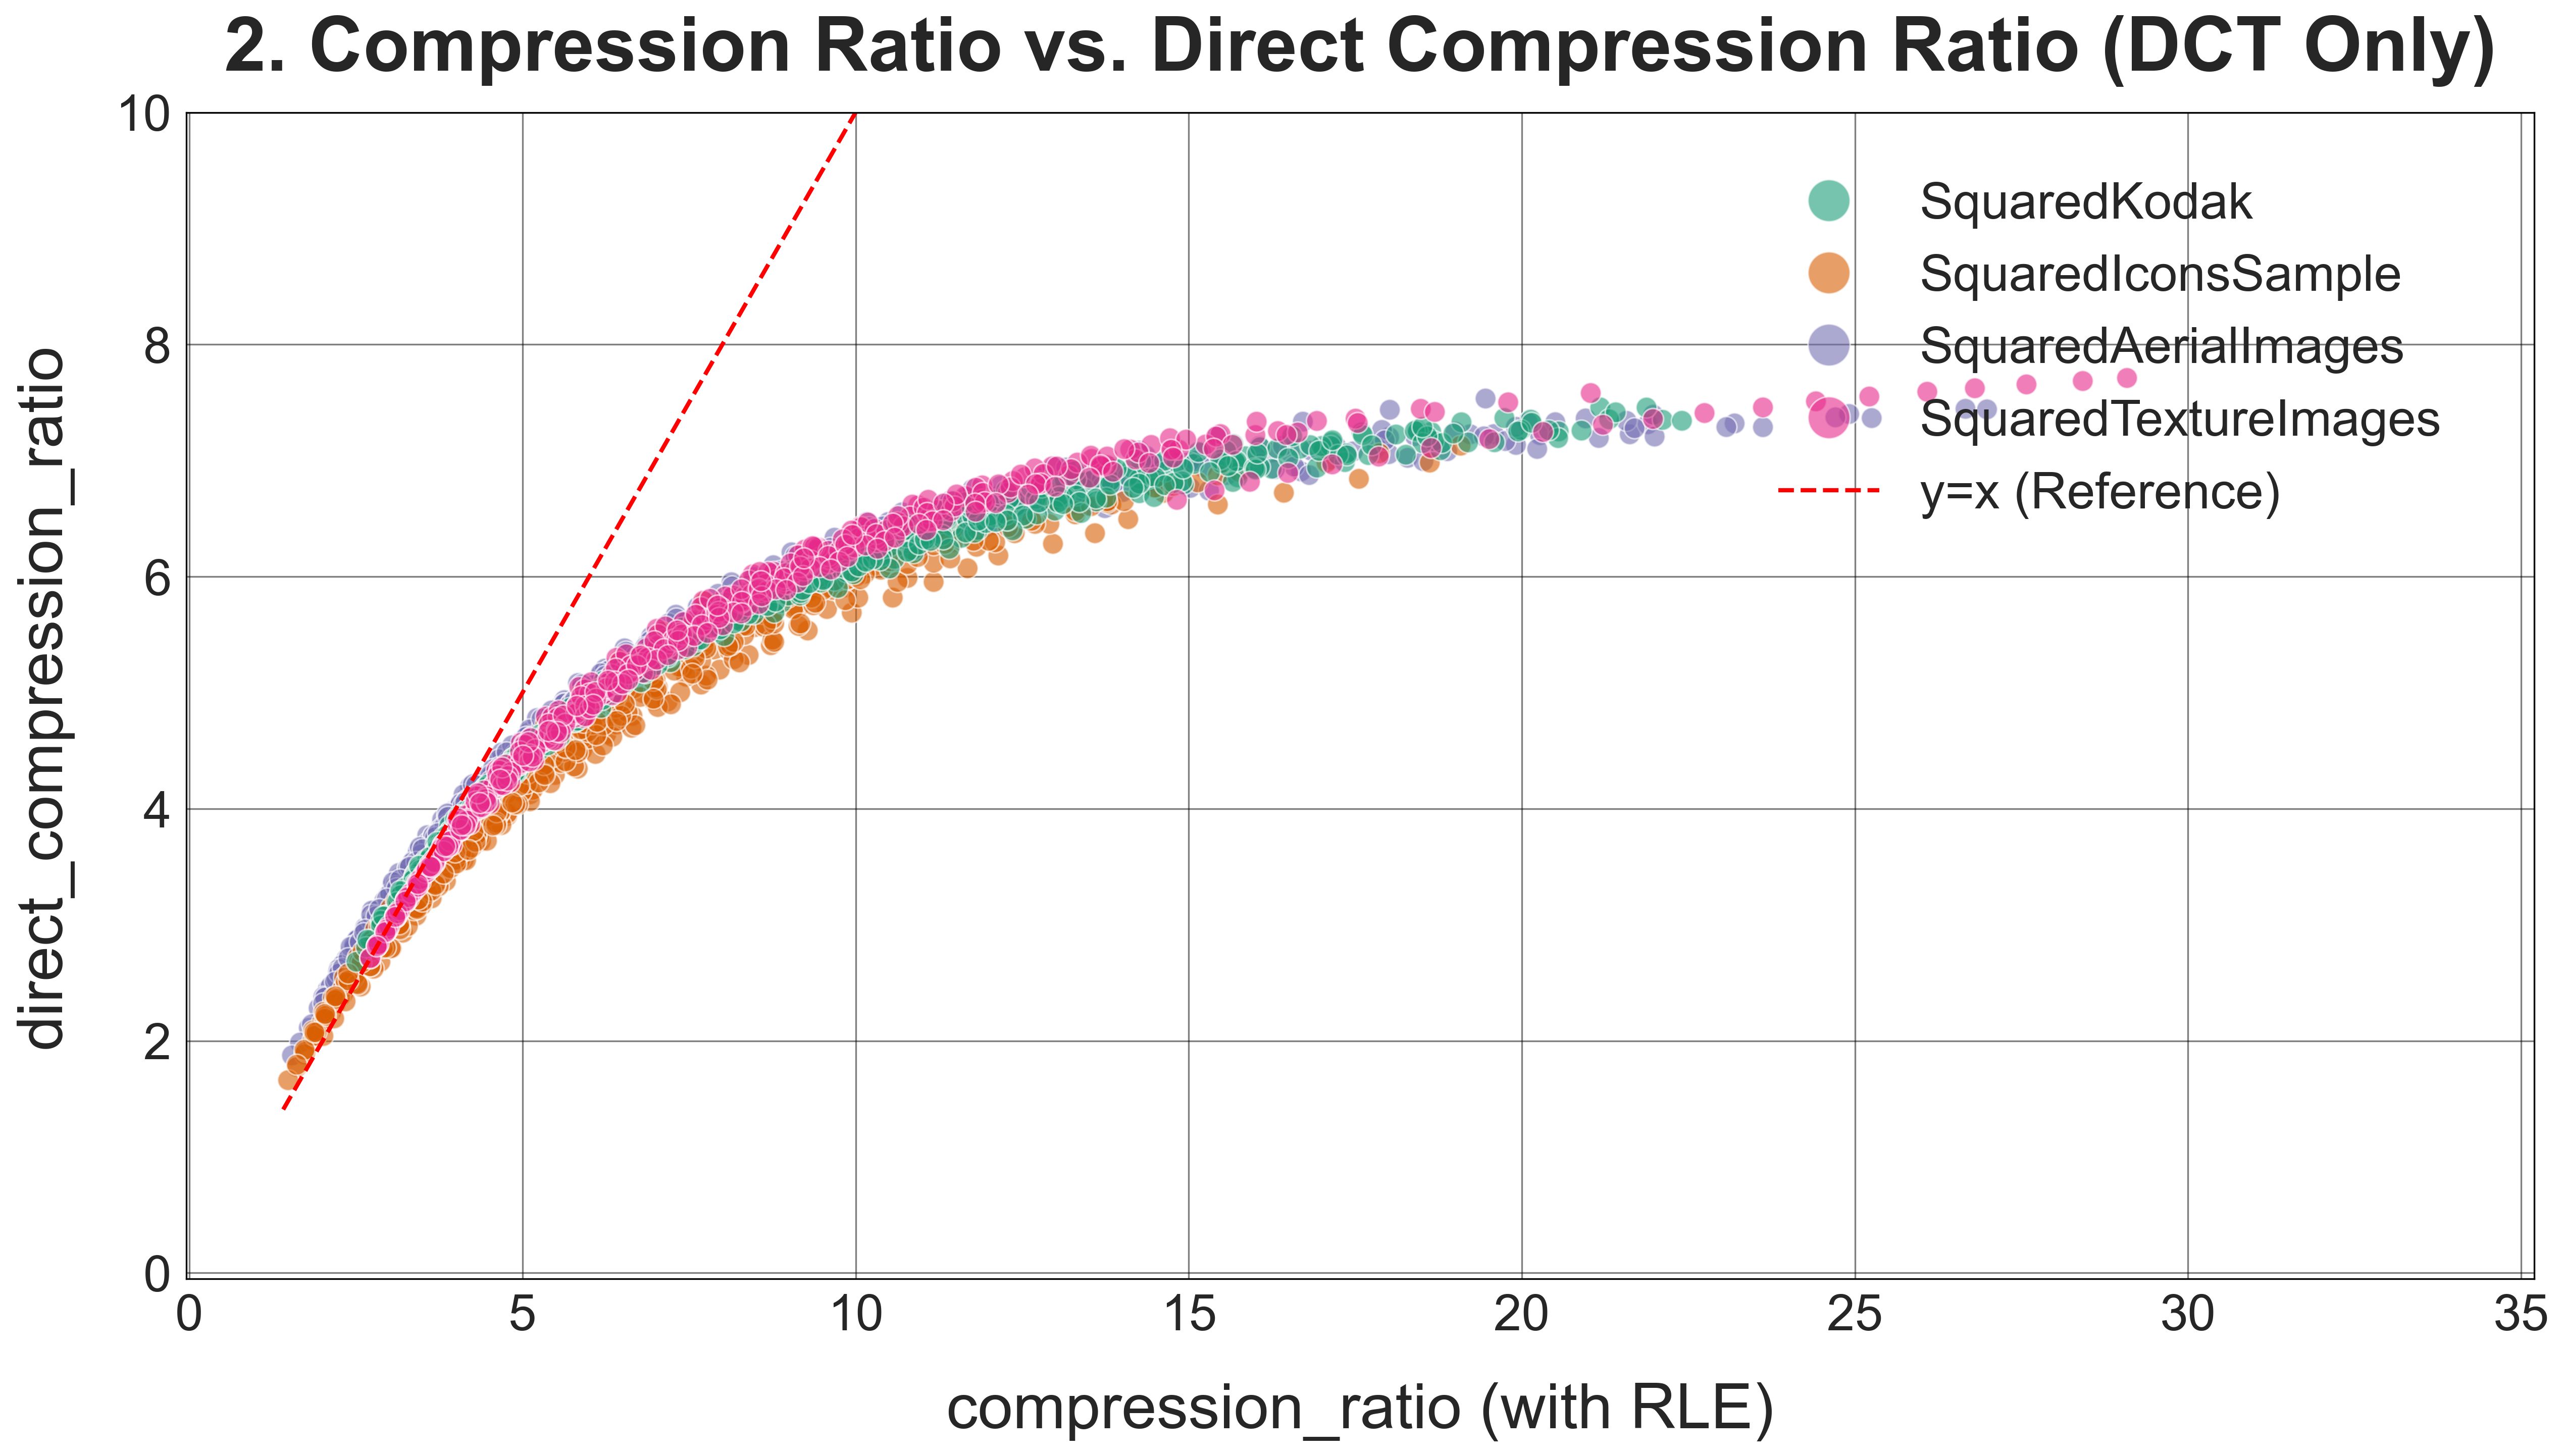
\includegraphics[width=1\linewidth]{results/plots/plot_6_cr_vs_direct_cr_DCT.png}
    \caption{Different levels of quantization on sample image with compression ratio.}
    \label{fig:dctcrvsdcr}
\end{figure}

This provides an excellent example of how compression algorithms can work together to achieve maximum compression for input data. Since the DCT is part of the well established JPEG pipeline, there are lots of extra tools to push the compression to the limit. Likely given more time, other techniques could be implemented to further improve algorithms like DWT and S+P as well.



We claimed in \ref{methodsec:fourier} that DCT is superior to DFT for image compression. To see this clearly, Fig. \ref{fig:dctvsdft} shows how DCT achieves much higher compression ratios at equivalent PSNR values across all datasets. For example, at a PSNR of 30 dB, the DFT achieves CR$\approx5$ across all datasets, while DCT has CR$\approx10$, even closer to 15 for Aerial Images. 

\begin{figure}
    \centering
    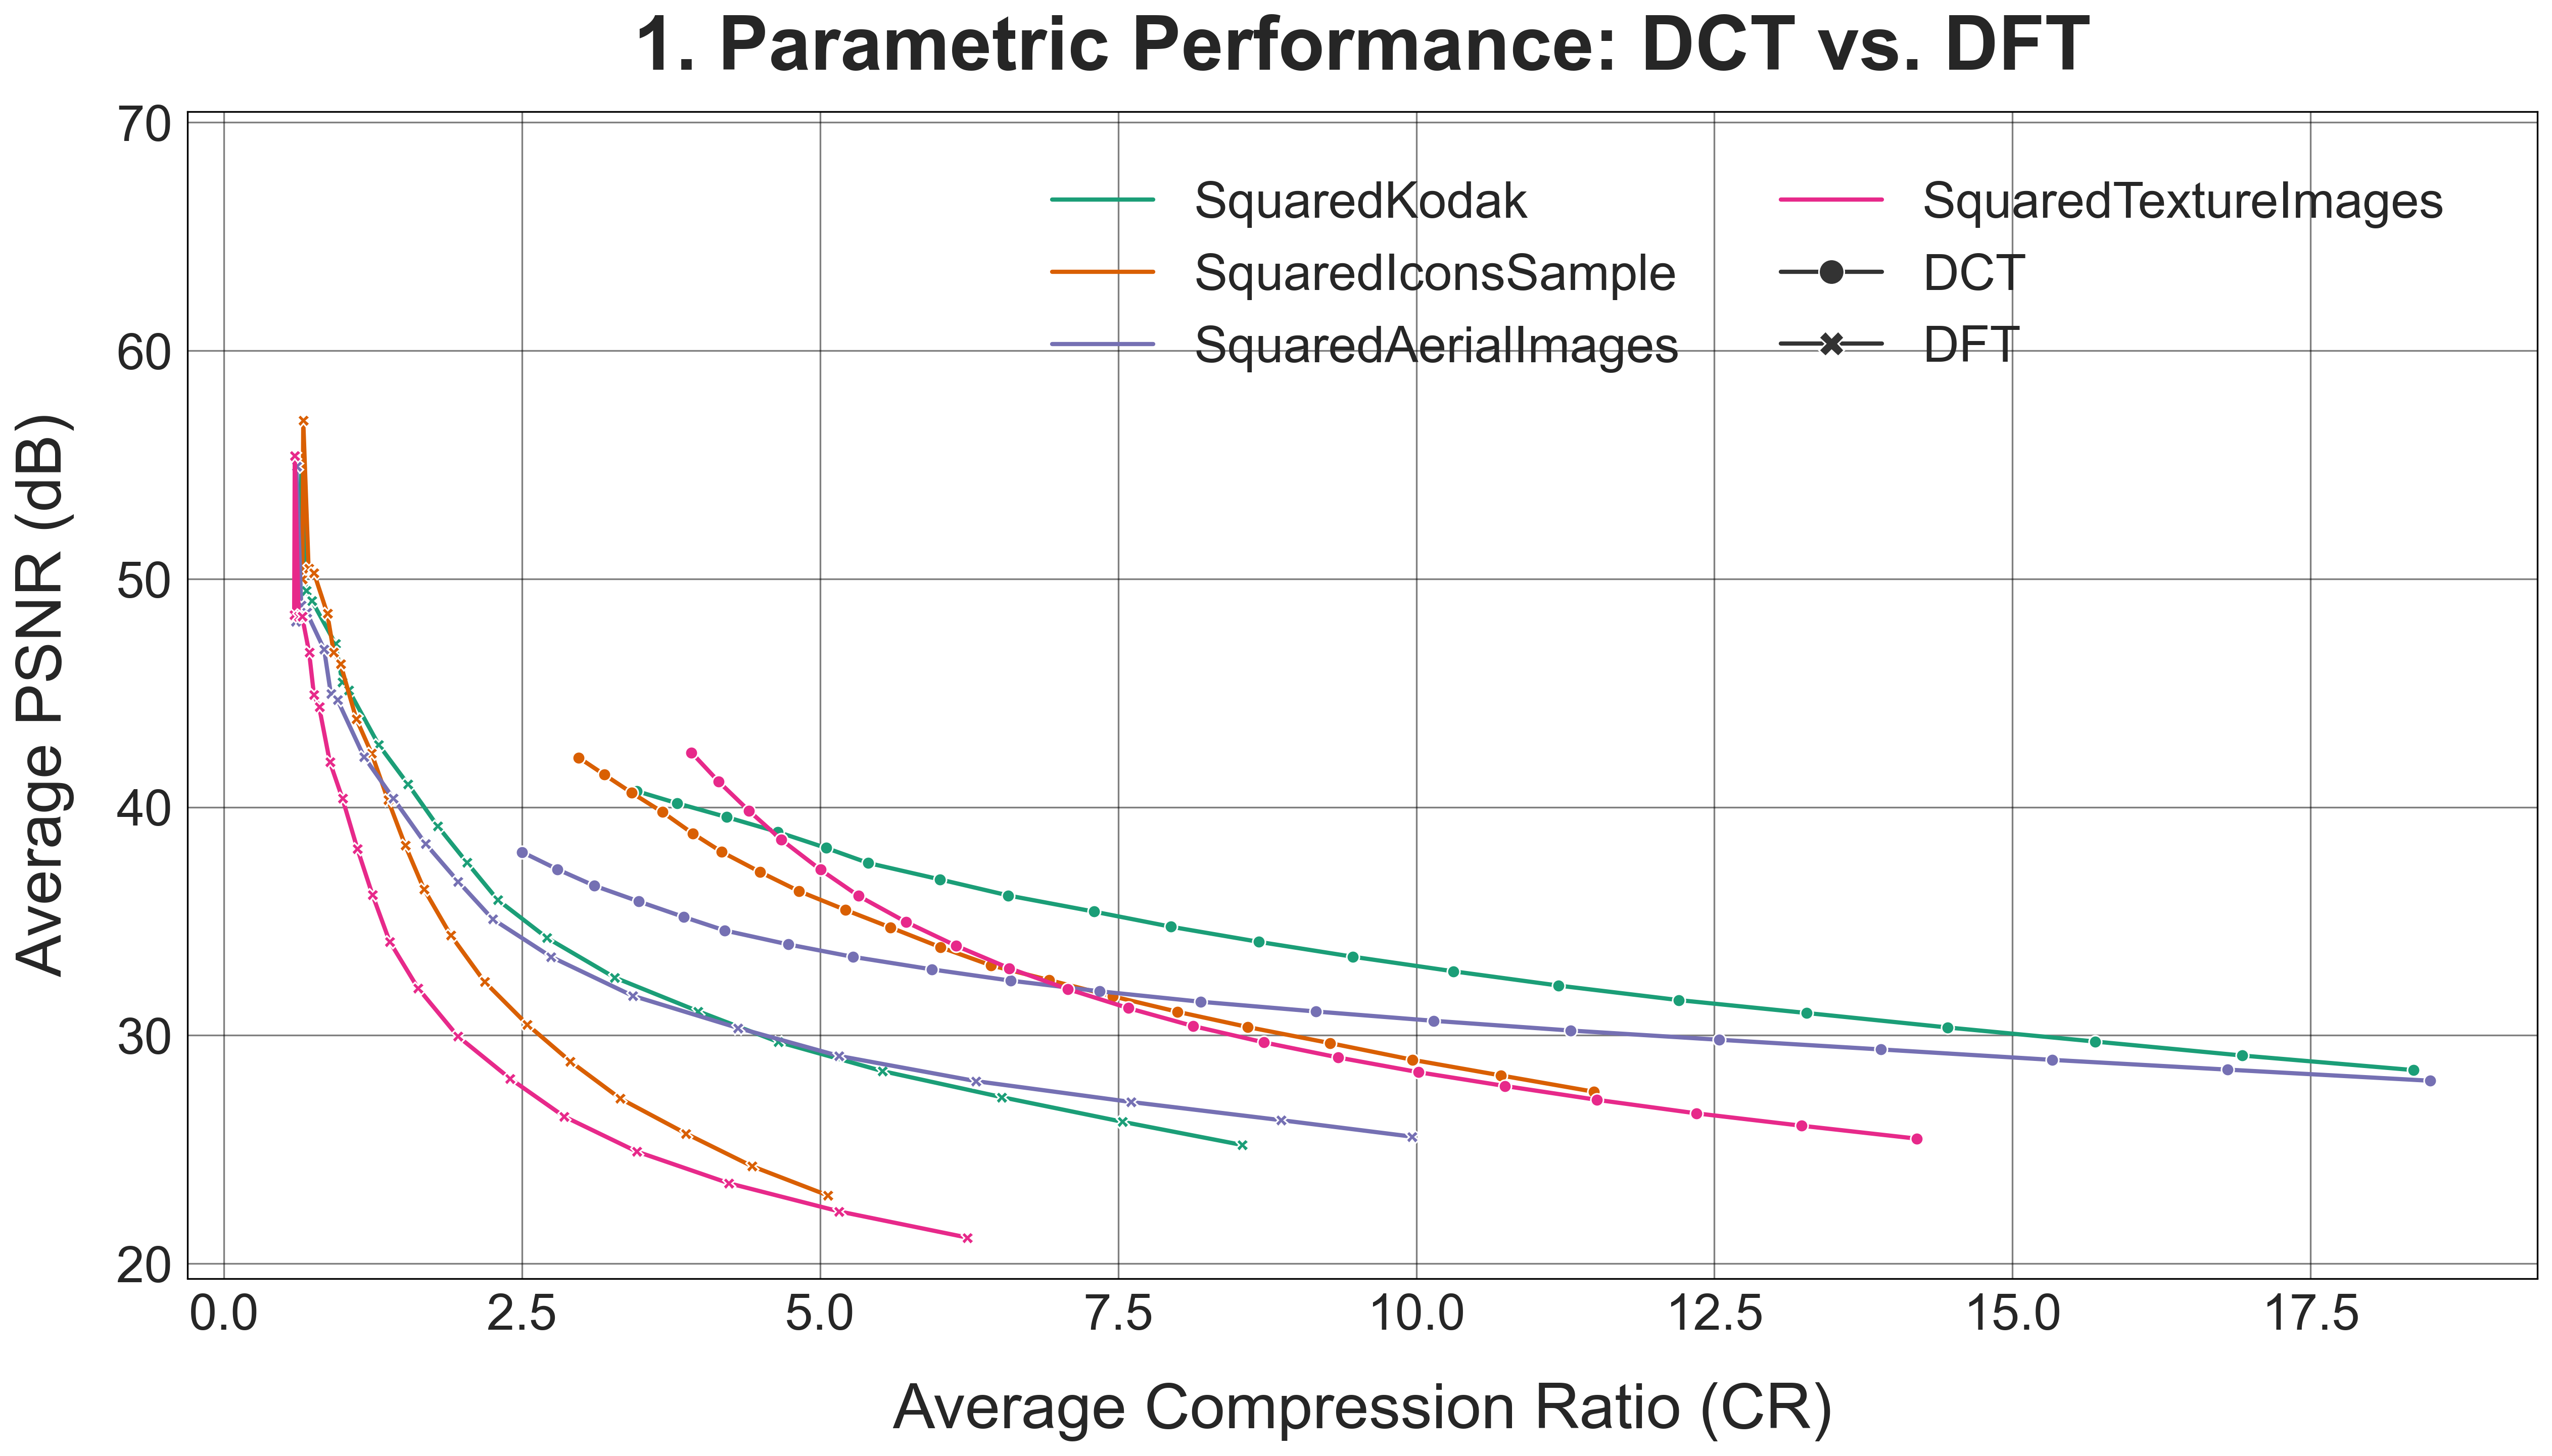
\includegraphics[width=1\linewidth]{results/plots/plot_5_parametric_DCT_vs_DFT.png}
    \caption{Different levels of quantization on sample image with compression ratio.}
    \label{fig:dctvsdft}
\end{figure}

Notably, in \ref{resultssec:col} it appears that the DCT outperforms all transform algorithms, not just the DFT. This comparison is slightly unfair since an additional step RLE was added to the entropy coding for DCT as described in \ref{methodsec:entropy}. Fig. \ref{fig:dctcrvsdcr} shows how the compression ratios change without RLE present for a more fair comparison.

\begin{figure}
    \centering
    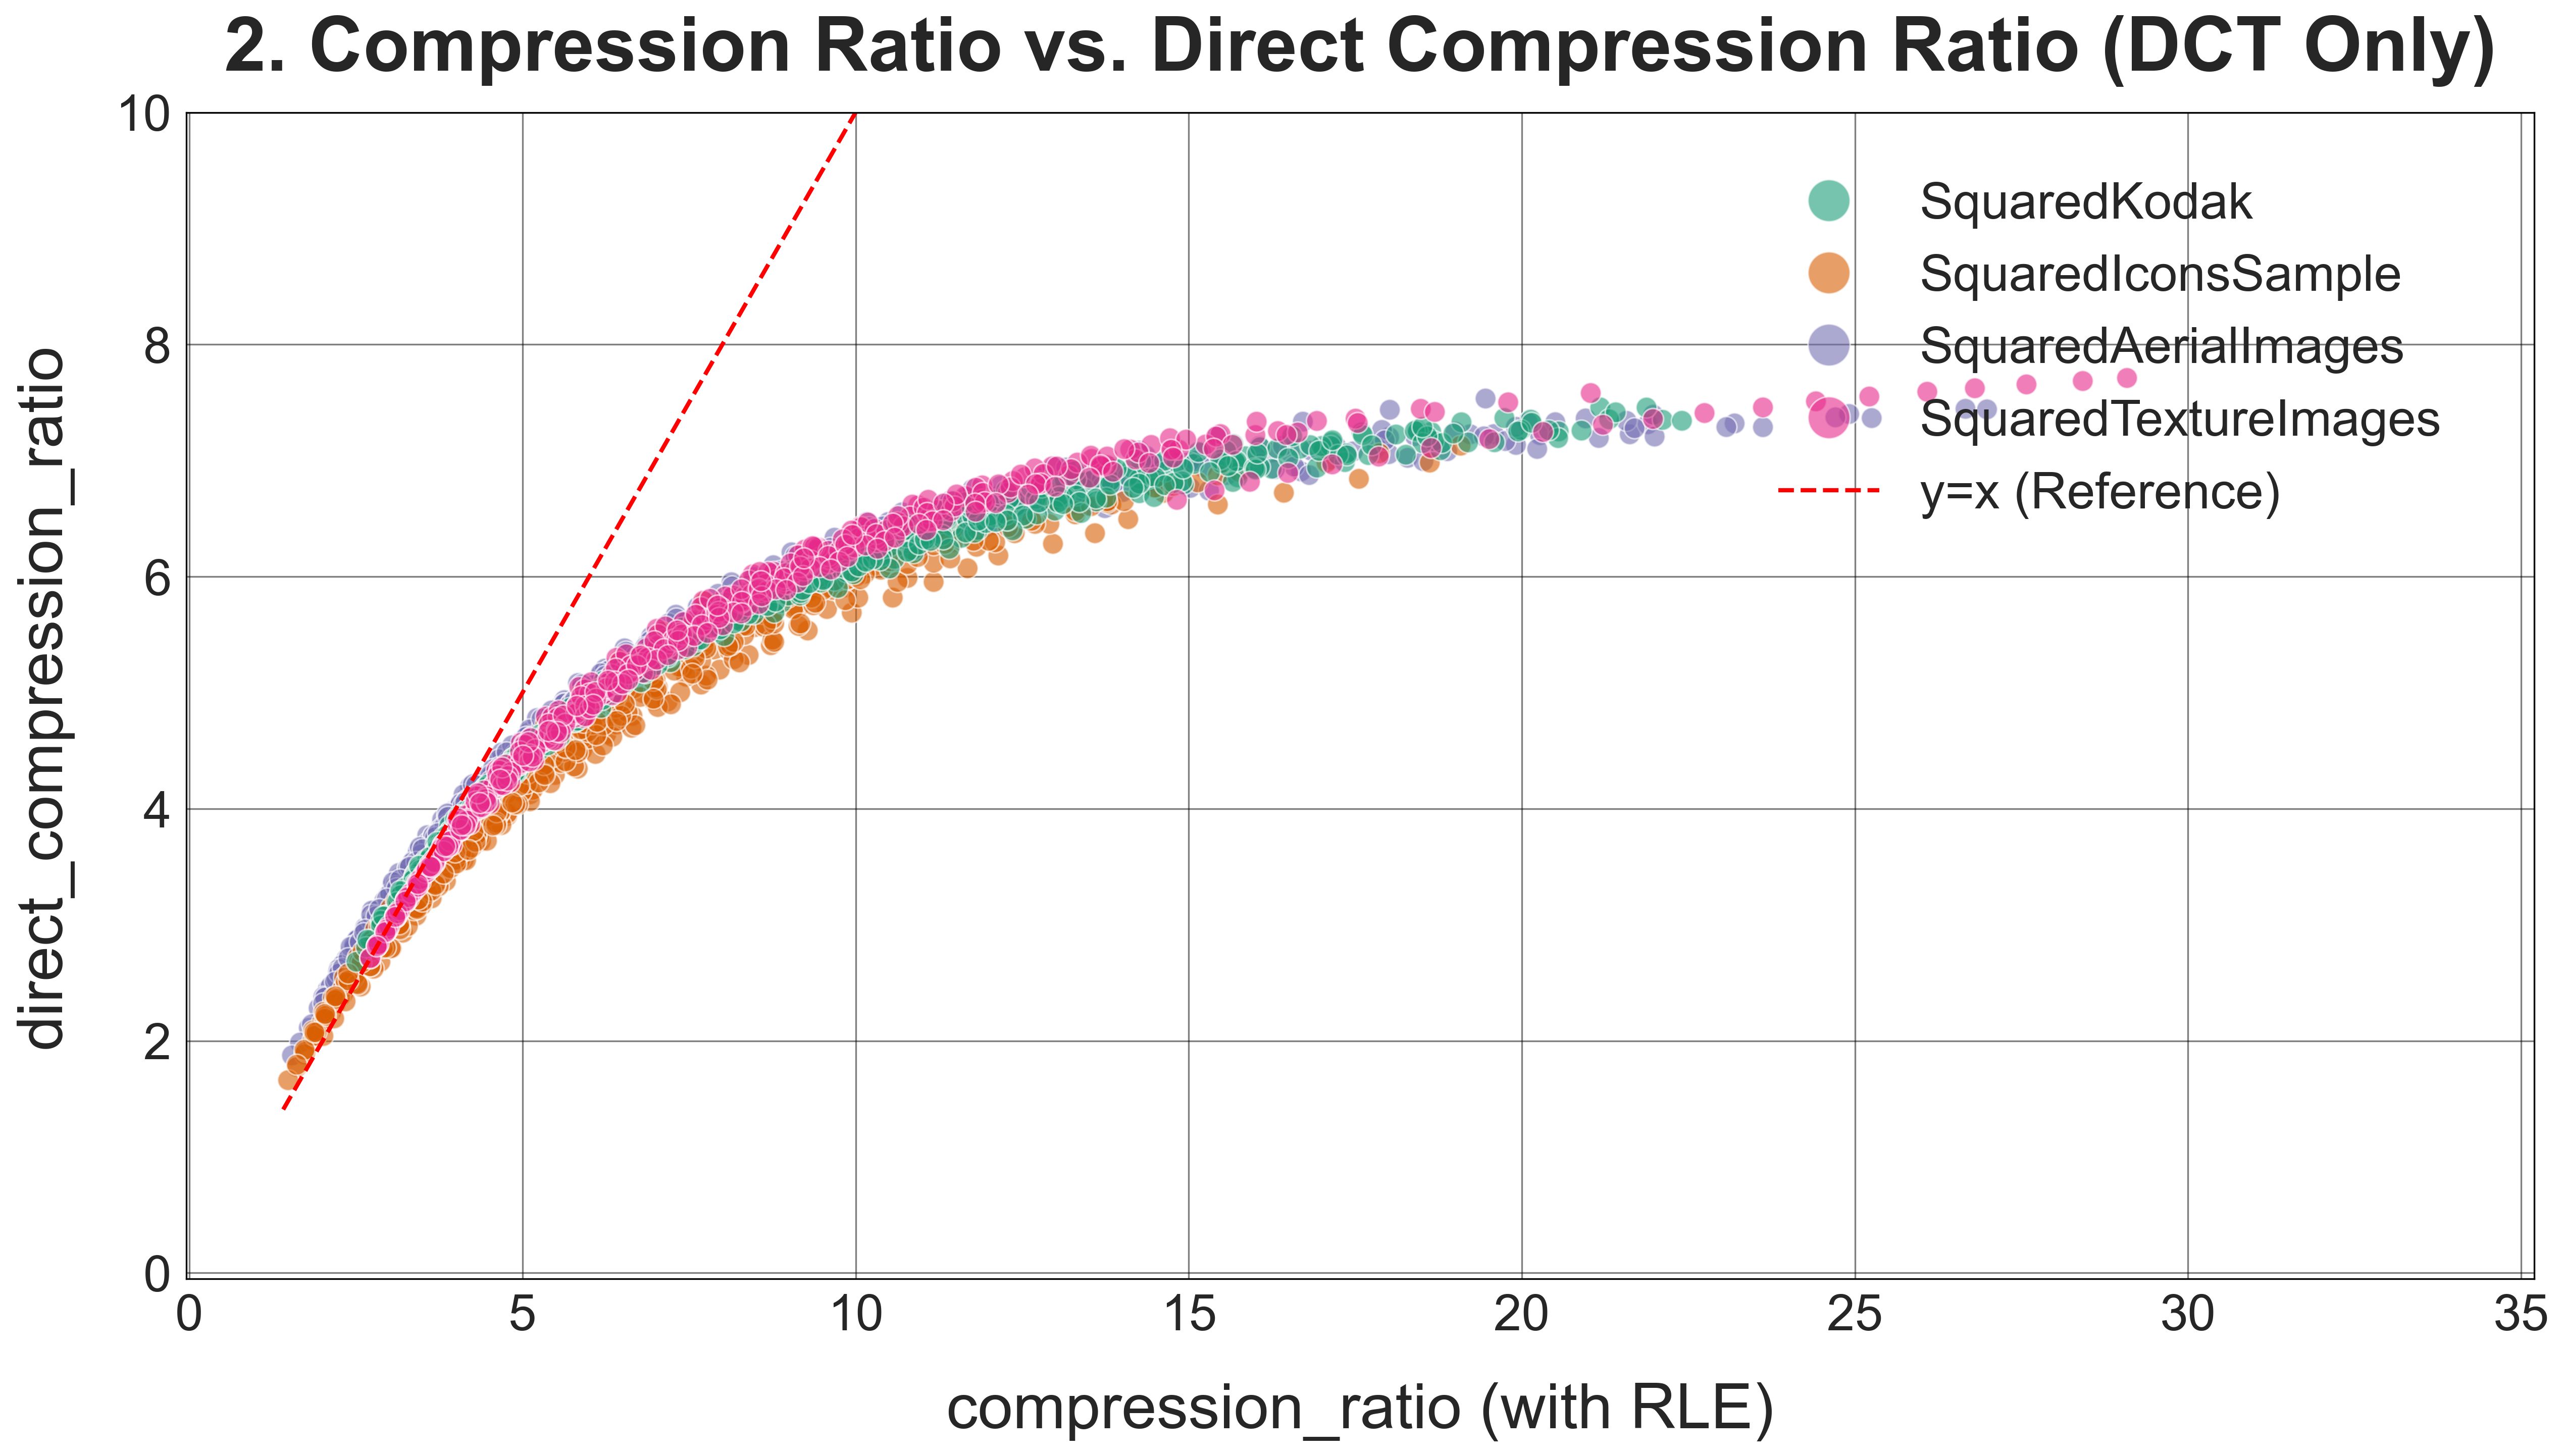
\includegraphics[width=1\linewidth]{results/plots/plot_6_cr_vs_direct_cr_DCT.png}
    \caption{Different levels of quantization on sample image with compression ratio.}
    \label{fig:dctcrvsdcr}
\end{figure}

This provides an excellent example of how compression algorithms can work together to achieve maximum compression for input data. Since the DCT is part of the well established JPEG pipeline, there are lots of extra tools to push the compression to the limit. Likely given more time, other techniques could be implemented to further improve algorithms like DWT and S+P as well.



We claimed in \ref{methodsec:fourier} that DCT is superior to DFT for image compression. To see this clearly, Fig. \ref{fig:dctvsdft} shows how DCT achieves much higher compression ratios at equivalent PSNR values across all datasets. For example, at a PSNR of 30 dB, the DFT achieves CR$\approx5$ across all datasets, while DCT has CR$\approx10$, even closer to 15 for Aerial Images. 

\begin{figure}
    \centering
    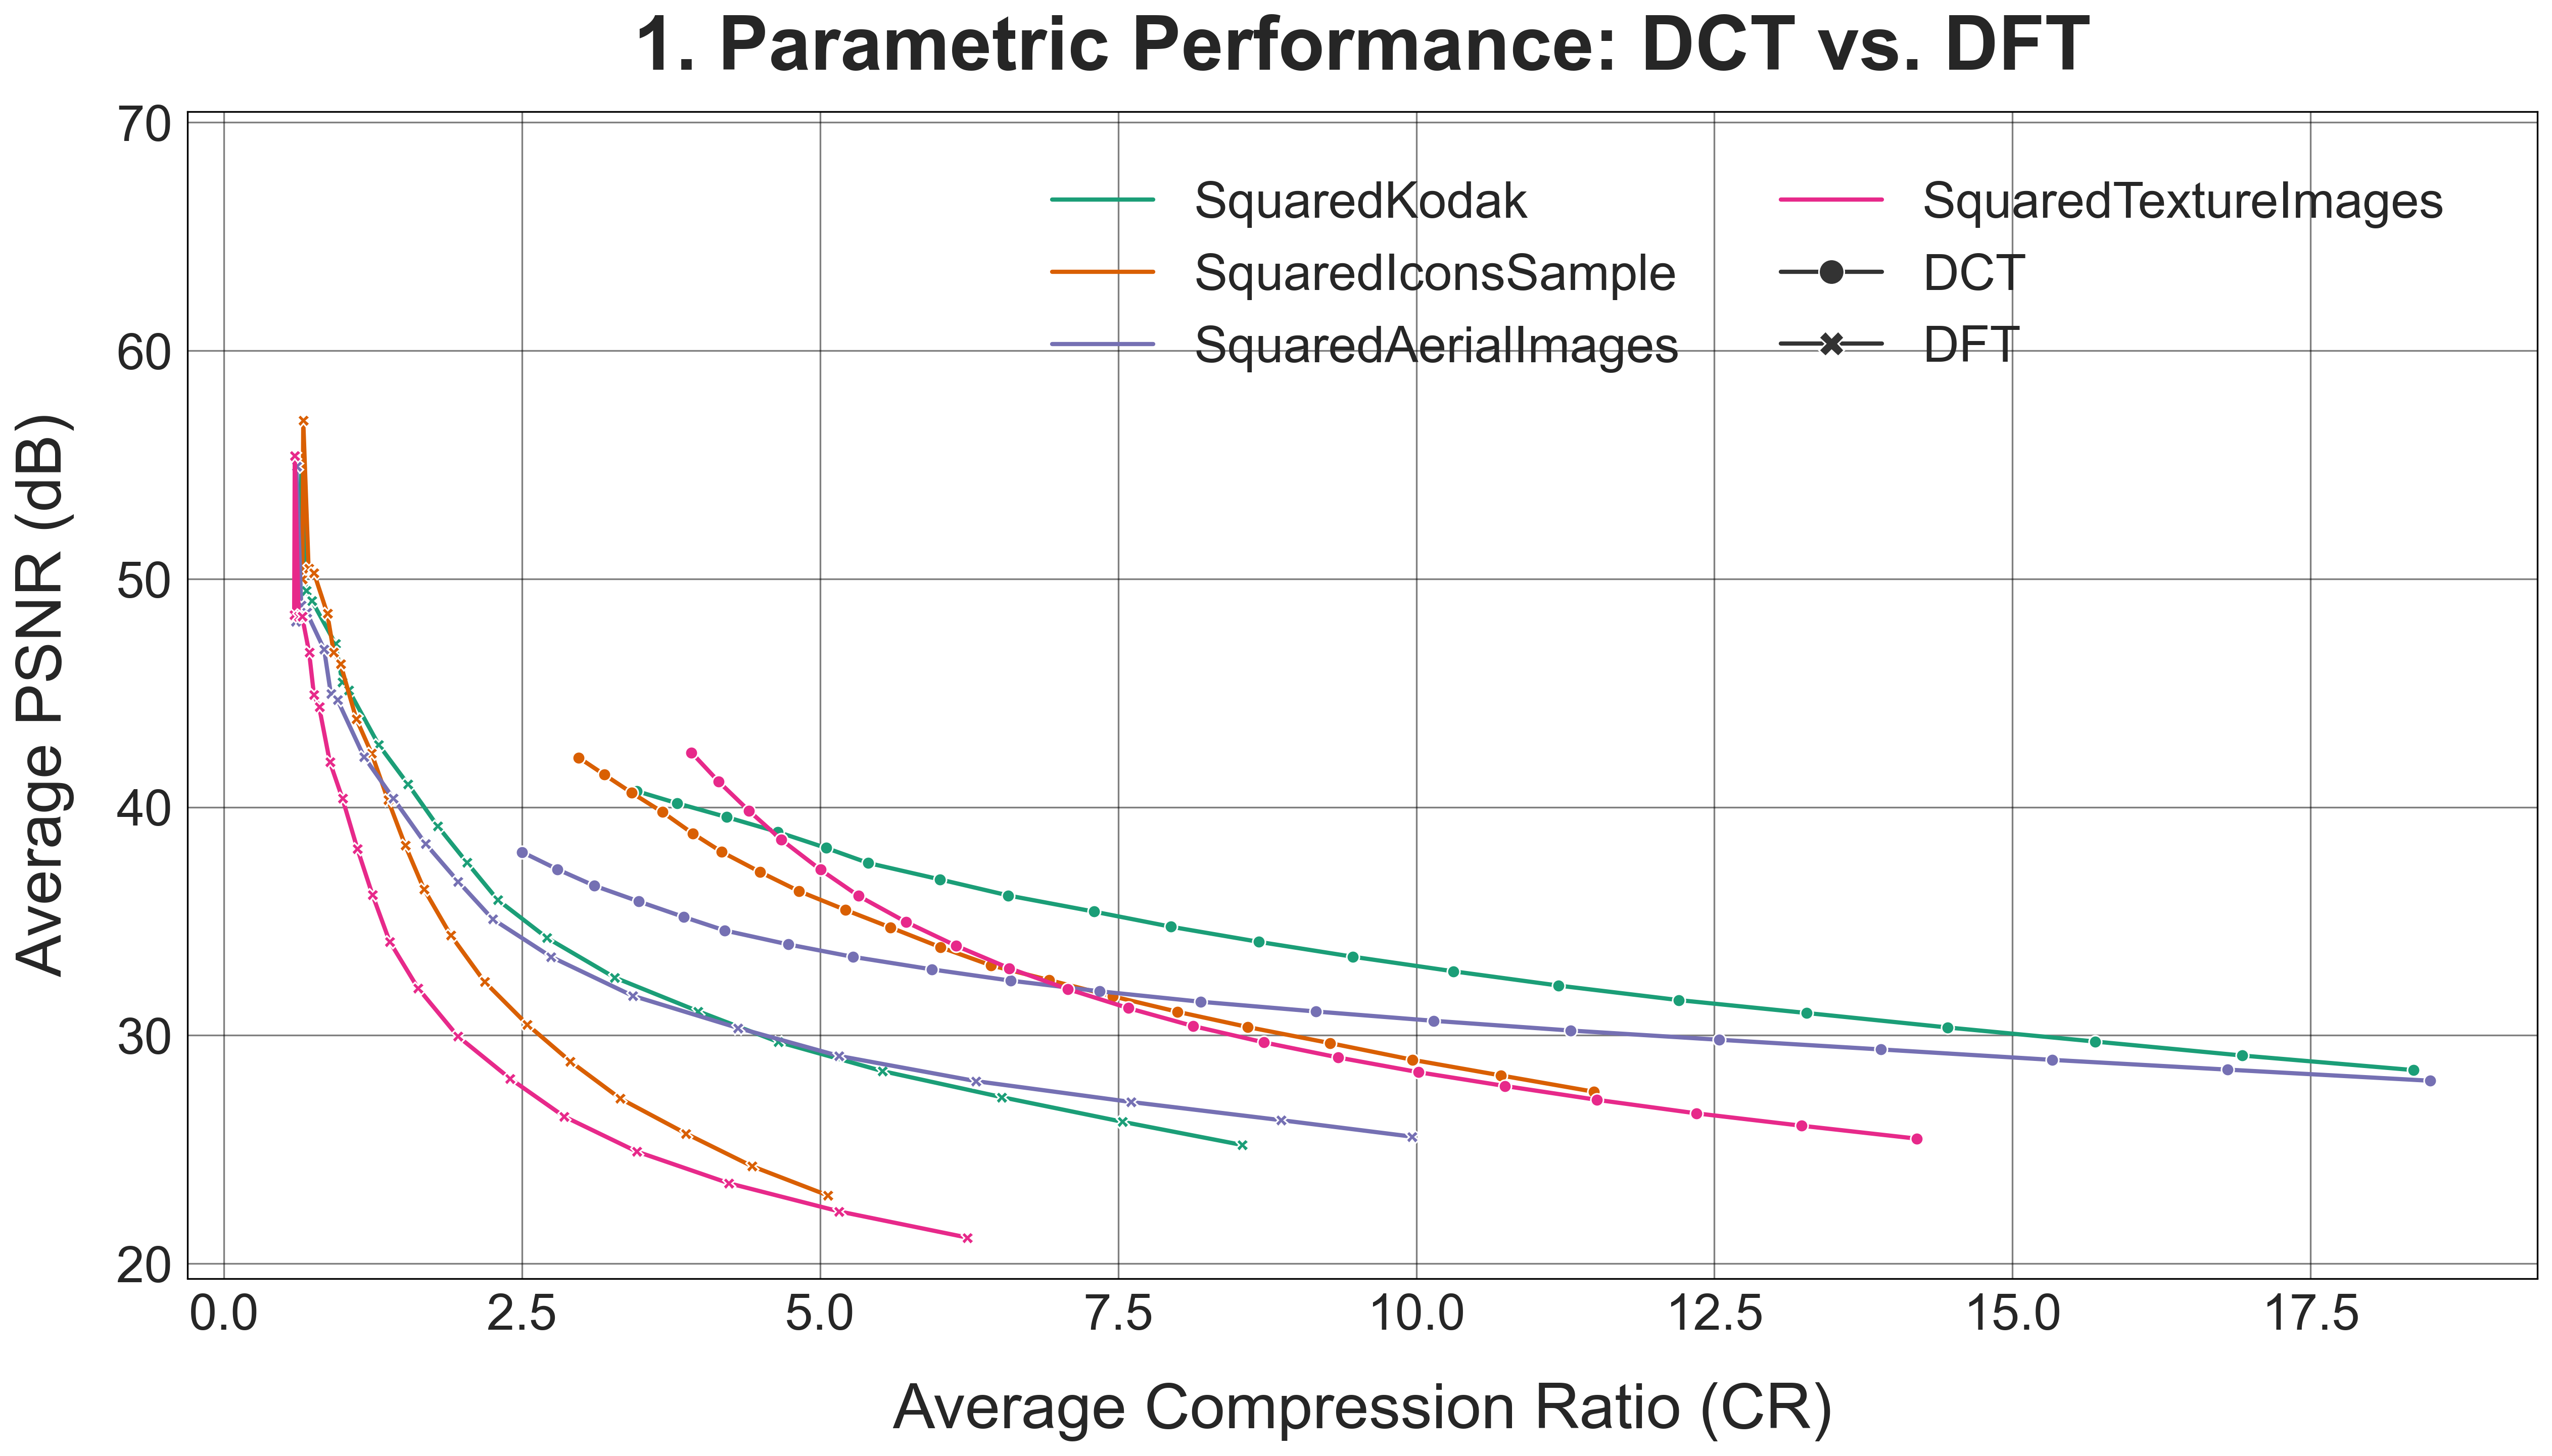
\includegraphics[width=1\linewidth]{results/plots/plot_5_parametric_DCT_vs_DFT.png}
    \caption{Different levels of quantization on sample image with compression ratio.}
    \label{fig:dctvsdft}
\end{figure}

Notably, in \ref{resultssec:col} it appears that the DCT outperforms all transform algorithms, not just the DFT. This comparison is slightly unfair since an additional step RLE was added to the entropy coding for DCT as described in \ref{methodsec:entropy}. Fig. \ref{fig:dctcrvsdcr} shows how the compression ratios change without RLE present for a more fair comparison.

\begin{figure}
    \centering
    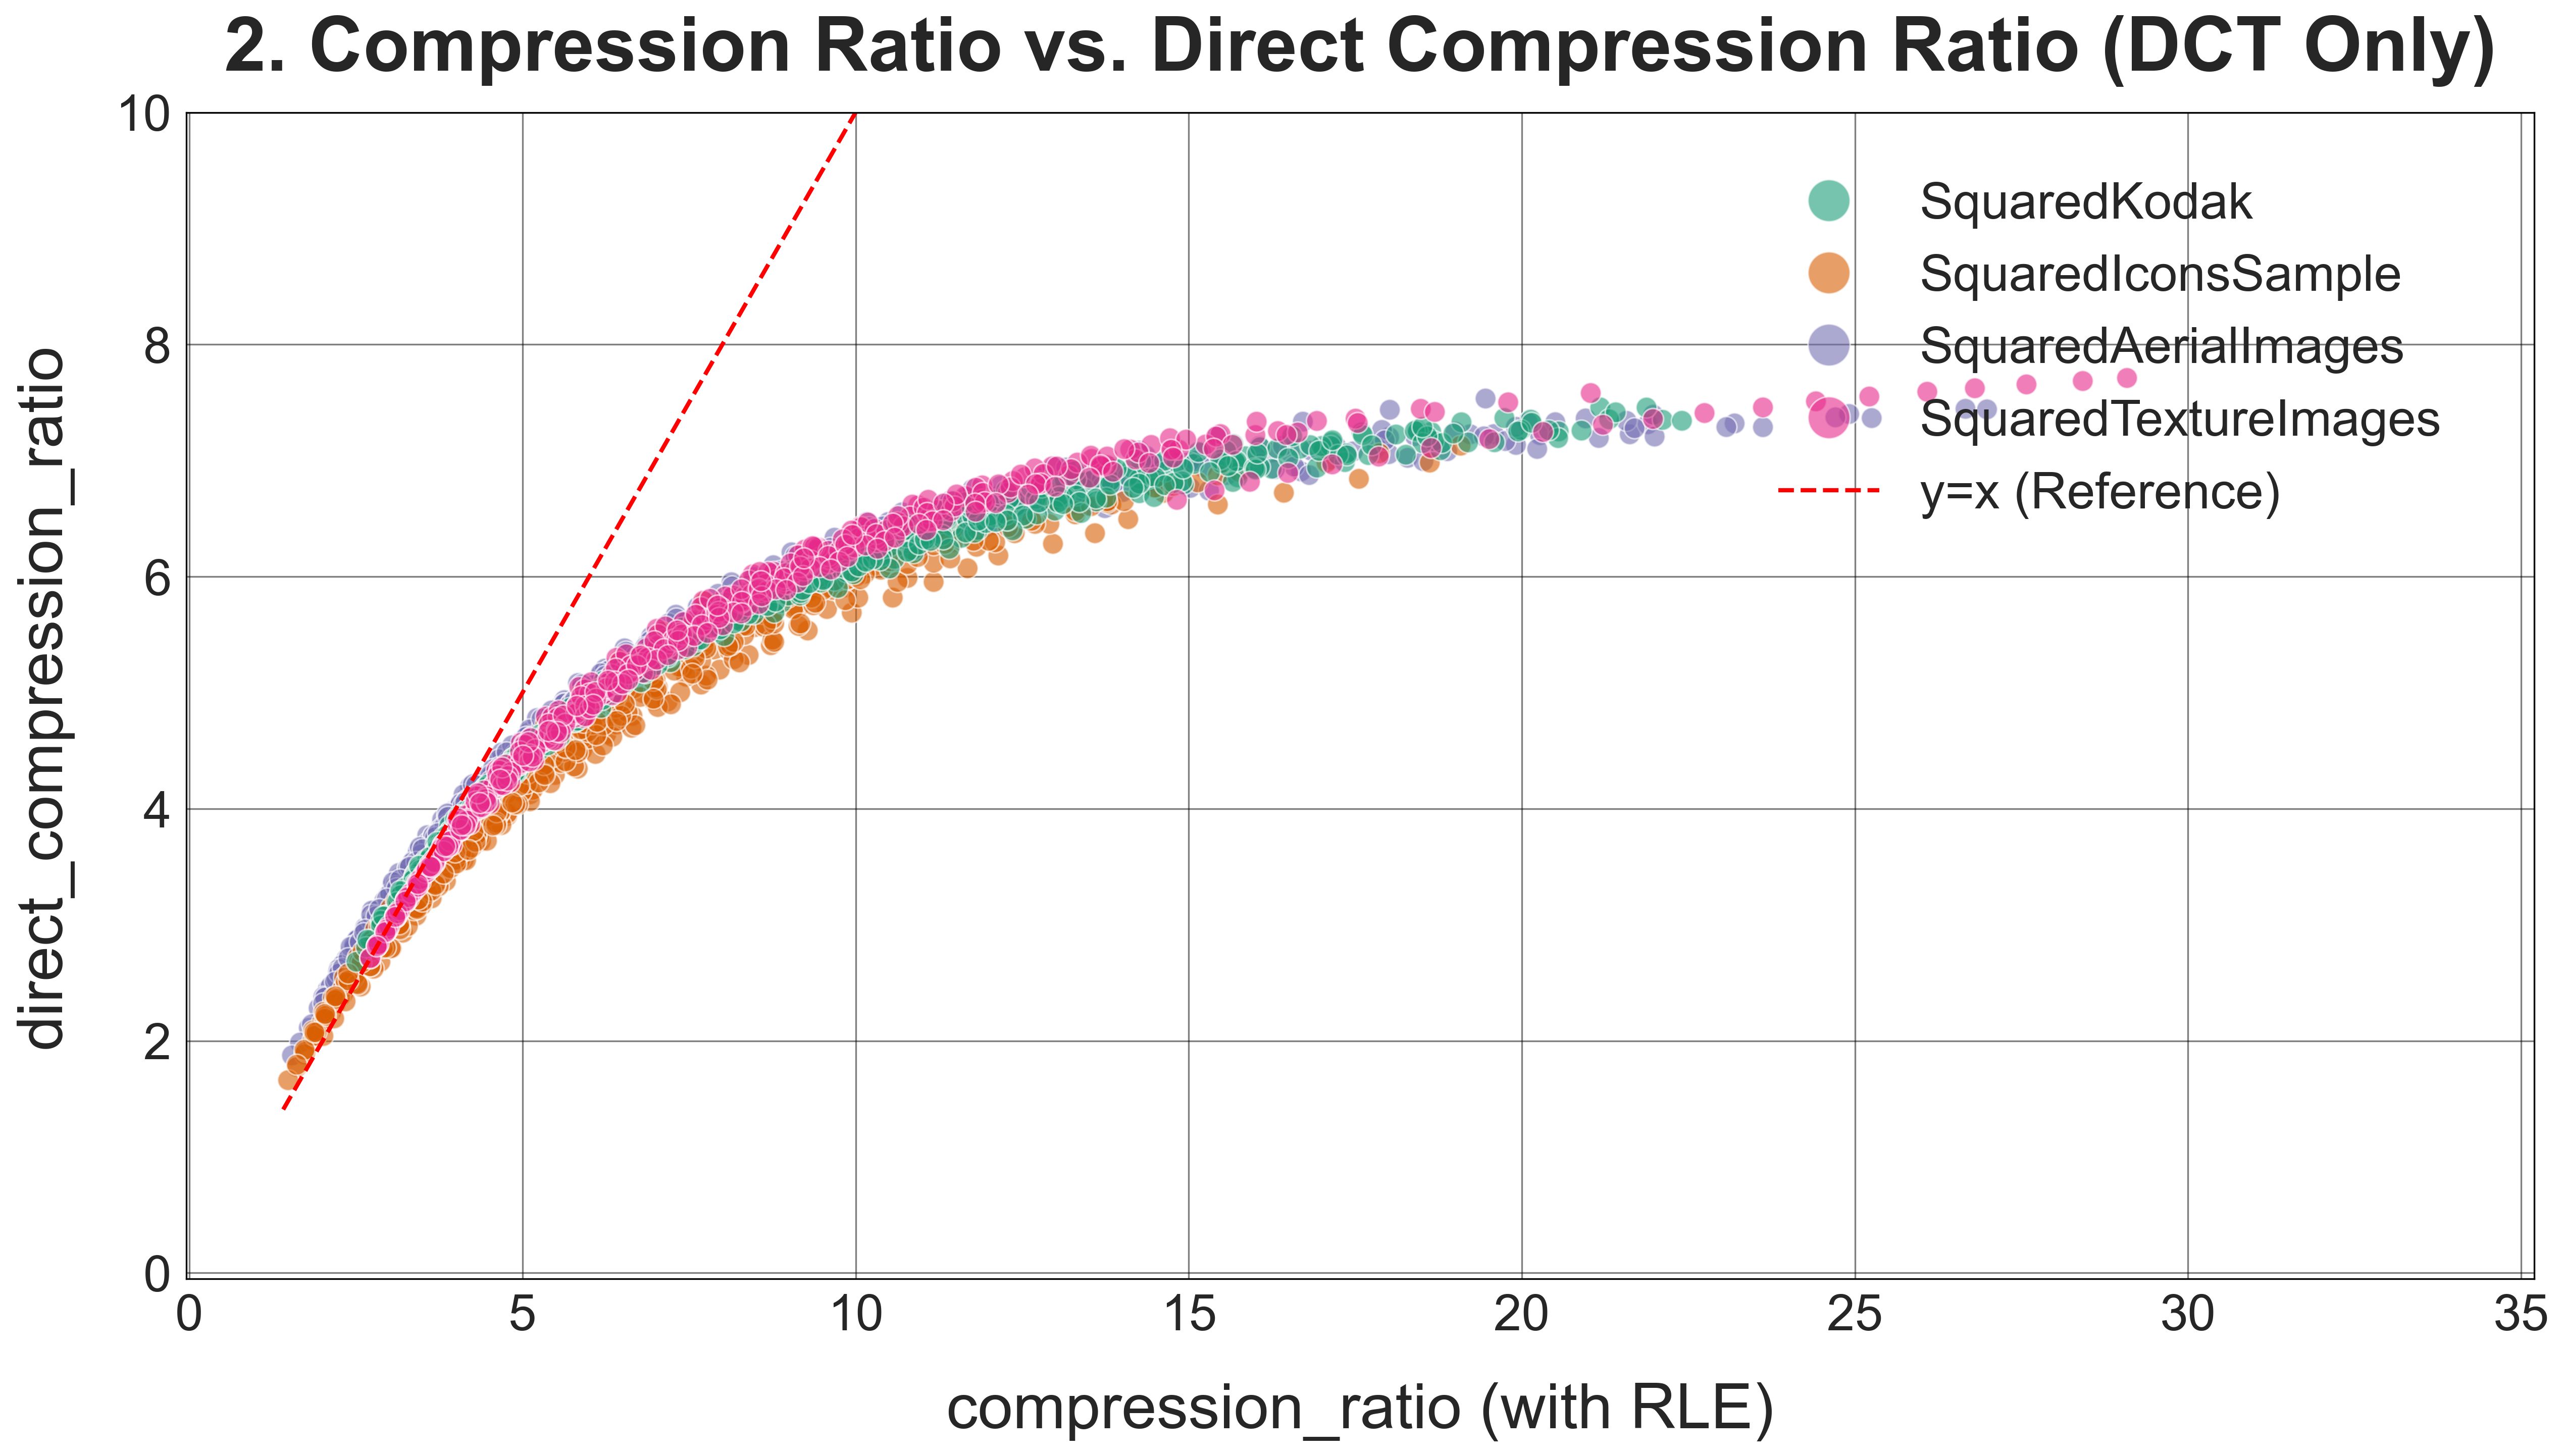
\includegraphics[width=1\linewidth]{results/plots/plot_6_cr_vs_direct_cr_DCT.png}
    \caption{Different levels of quantization on sample image with compression ratio.}
    \label{fig:dctcrvsdcr}
\end{figure}

This provides an excellent example of how compression algorithms can work together to achieve maximum compression for input data. Since the DCT is part of the well established JPEG pipeline, there are lots of extra tools to push the compression to the limit. Likely given more time, other techniques could be implemented to further improve algorithms like DWT and S+P as well.




\subsection{S+P Results}
\label{resultssec:sp}

Fig.~\ref{fig:sp_parametric} shows, for each squared dataset, the average PSNR
(in dB) as a function of the average compression ratio (CR) obtained by sweeping
the S+P quantization scale. As expected, all four curves exhibit a monotone
tradeoff: increasing CR is accompanied by decreasing PSNR. The datasets,
however, occupy different regions of the CR axis. Kodak, AerialImages, and
TextureImages all span roughly CR~$\approx 2$--$8$, whereas IconsSample is
confined to about CR~$\approx 1.7$--$6$, reflecting that these very small,
simple images cannot be pushed to the same nominal compression ratios.
\begin{figure}
    \centering
    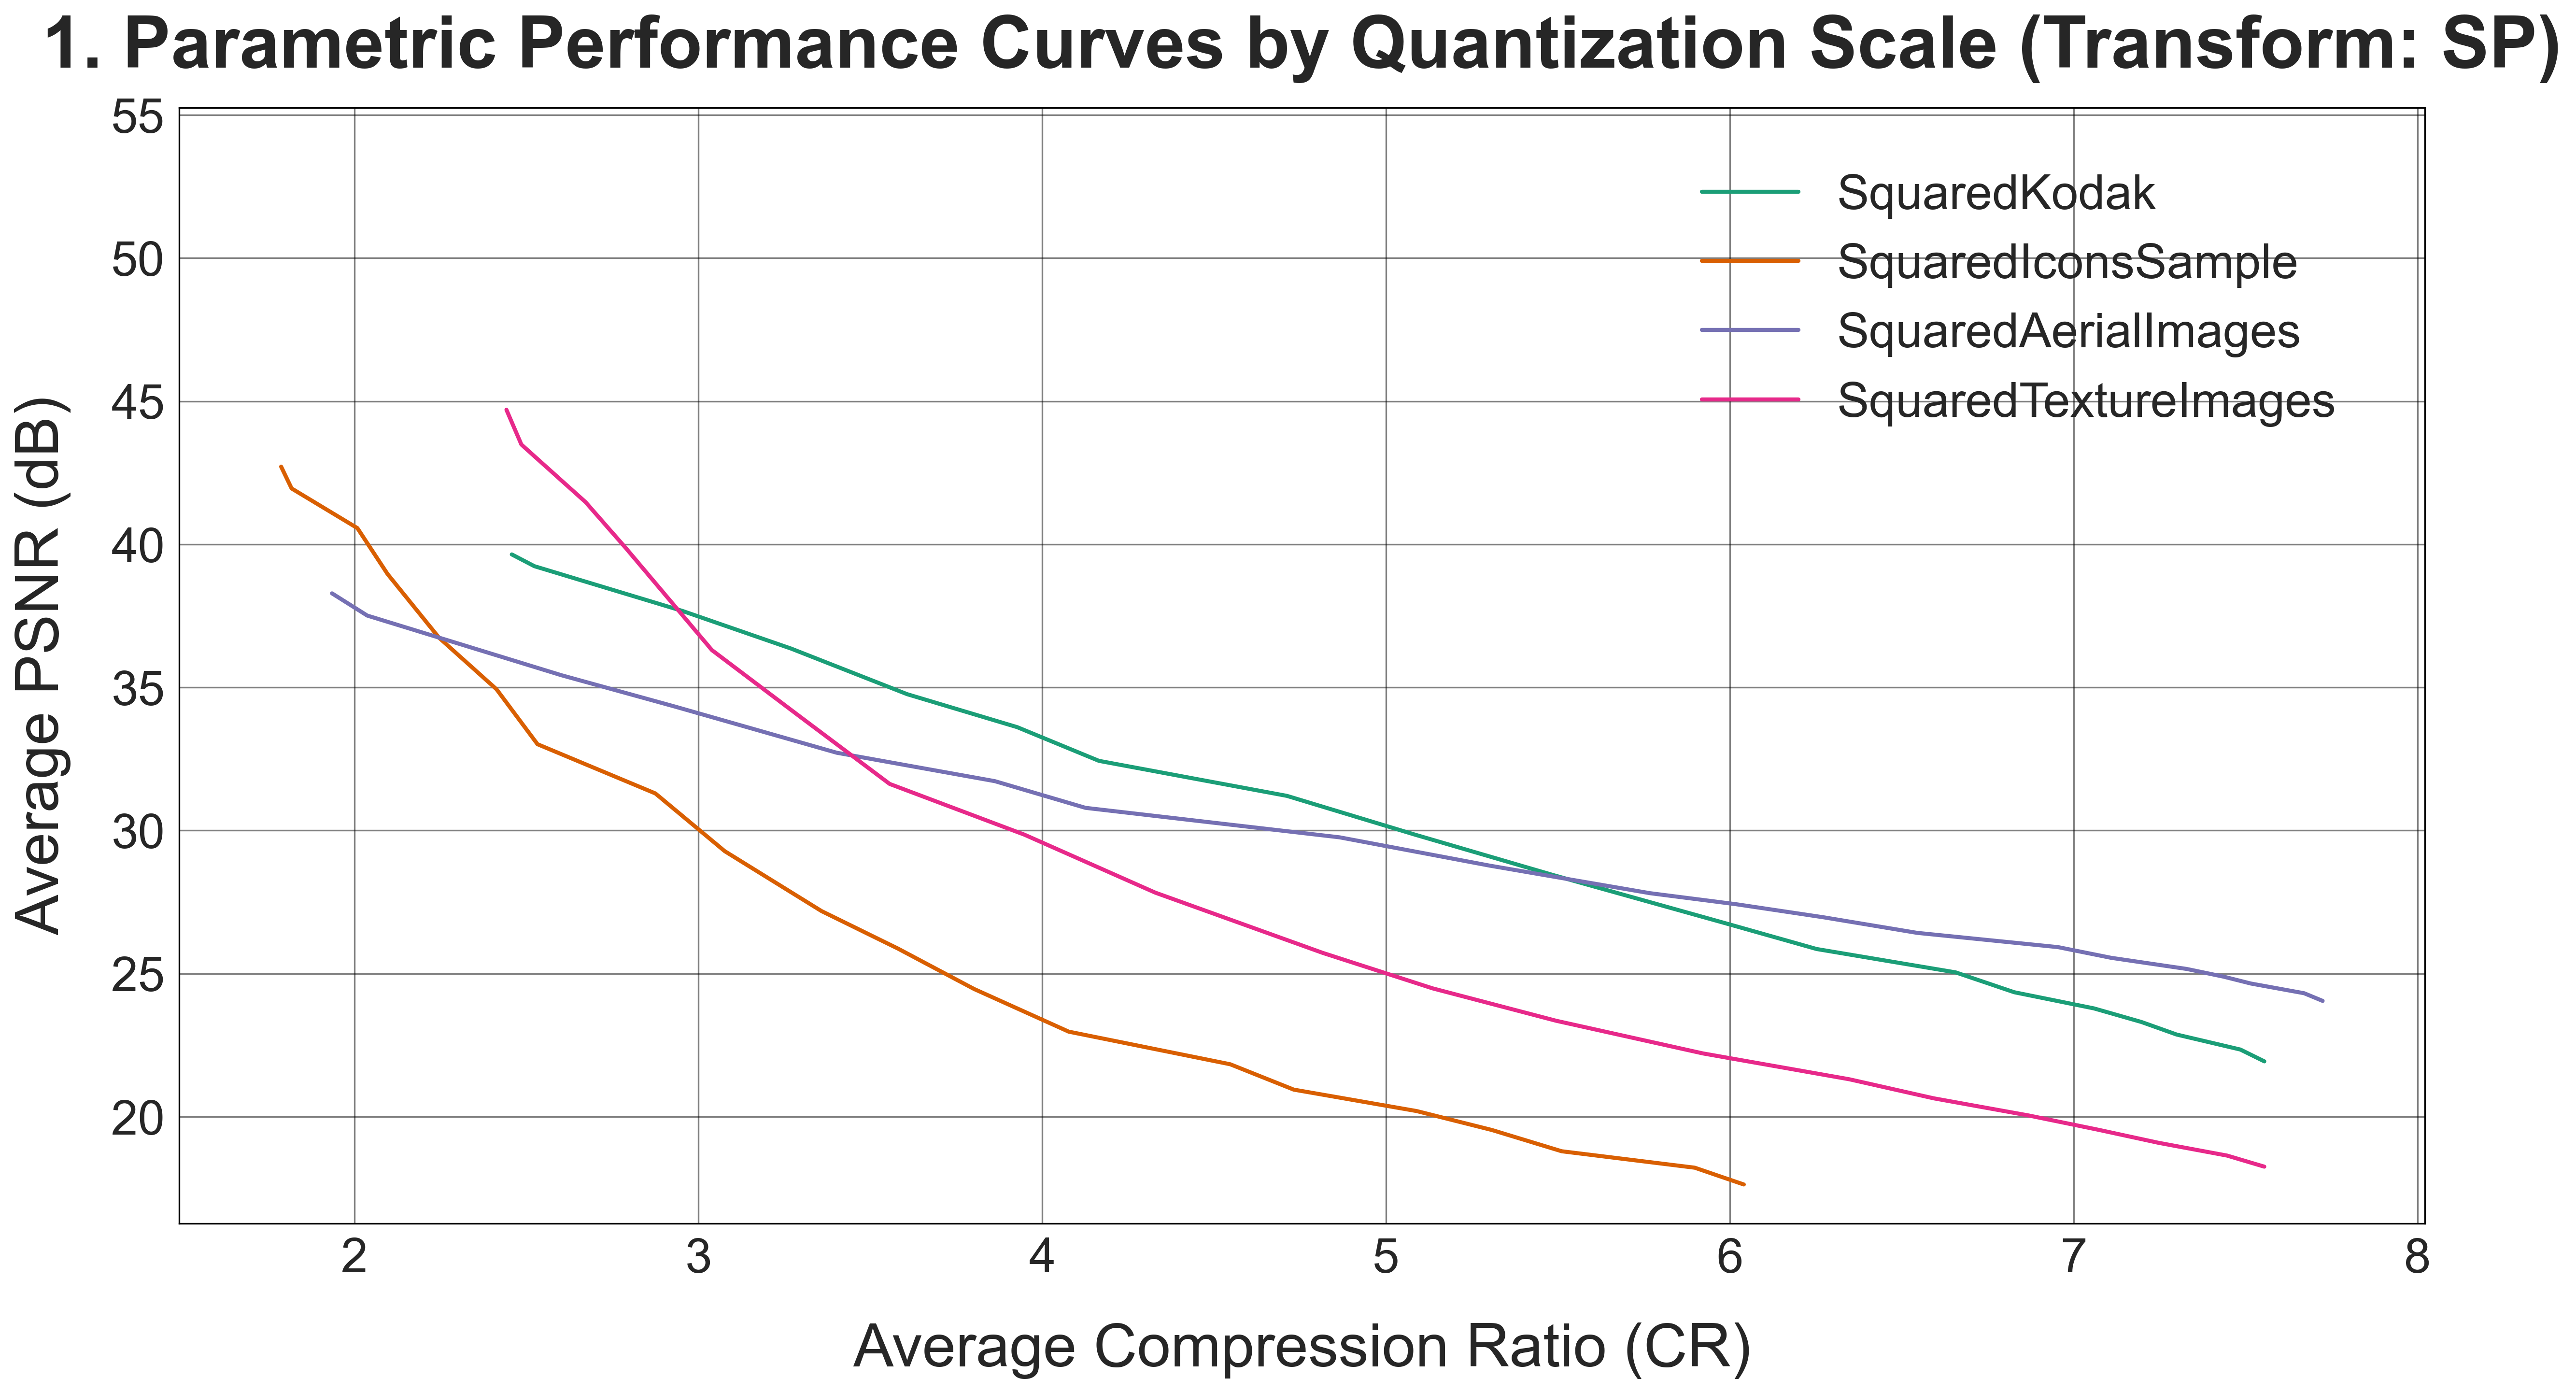
\includegraphics[width=1\linewidth]{results/plots/plot_1_parametric_curve_SP.png}
    \caption{S+P parametric performance: average PSNR vs.\ average compression ratio.}
    \label{fig:sp_parametric}
\end{figure}
At the low-CR end (around CR~$\approx 2$), TextureImages achieves the highest
average PSNR (around 45\,dB), with IconsSample close behind, and Kodak and
AerialImages clustered around 38--39\,dB. As CR increases, all curves slope
downward, but with noticeably different steepness. The Kodak and AerialImages
curves remain relatively close together, maintaining PSNR in the low
30\,dB range at CR~$\approx 4$ and still above 25\,dB at CR~$\approx 7$.
TextureImages falls somewhat faster but stays competitive through most of the
range. IconsSample begins near the top-left of the plot with high PSNR at
low CR, but its curve is the steepest: by CR~$\approx 5$ it has dropped to
around 20\,dB, and it does not extend into the very high-CR regime where the
other datasets continue.

Overall, these curves show that S+P exhibits the same dataset ordering
we observed in the Collective Results, with natural-image datasets clustering
together and IconsSample behaving as a low-CR, high-PSNR regime.
% providing a
% clear baseline for our direct comparison between S+P and Haar in the next
% section.

\begin{figure}
    \centering
    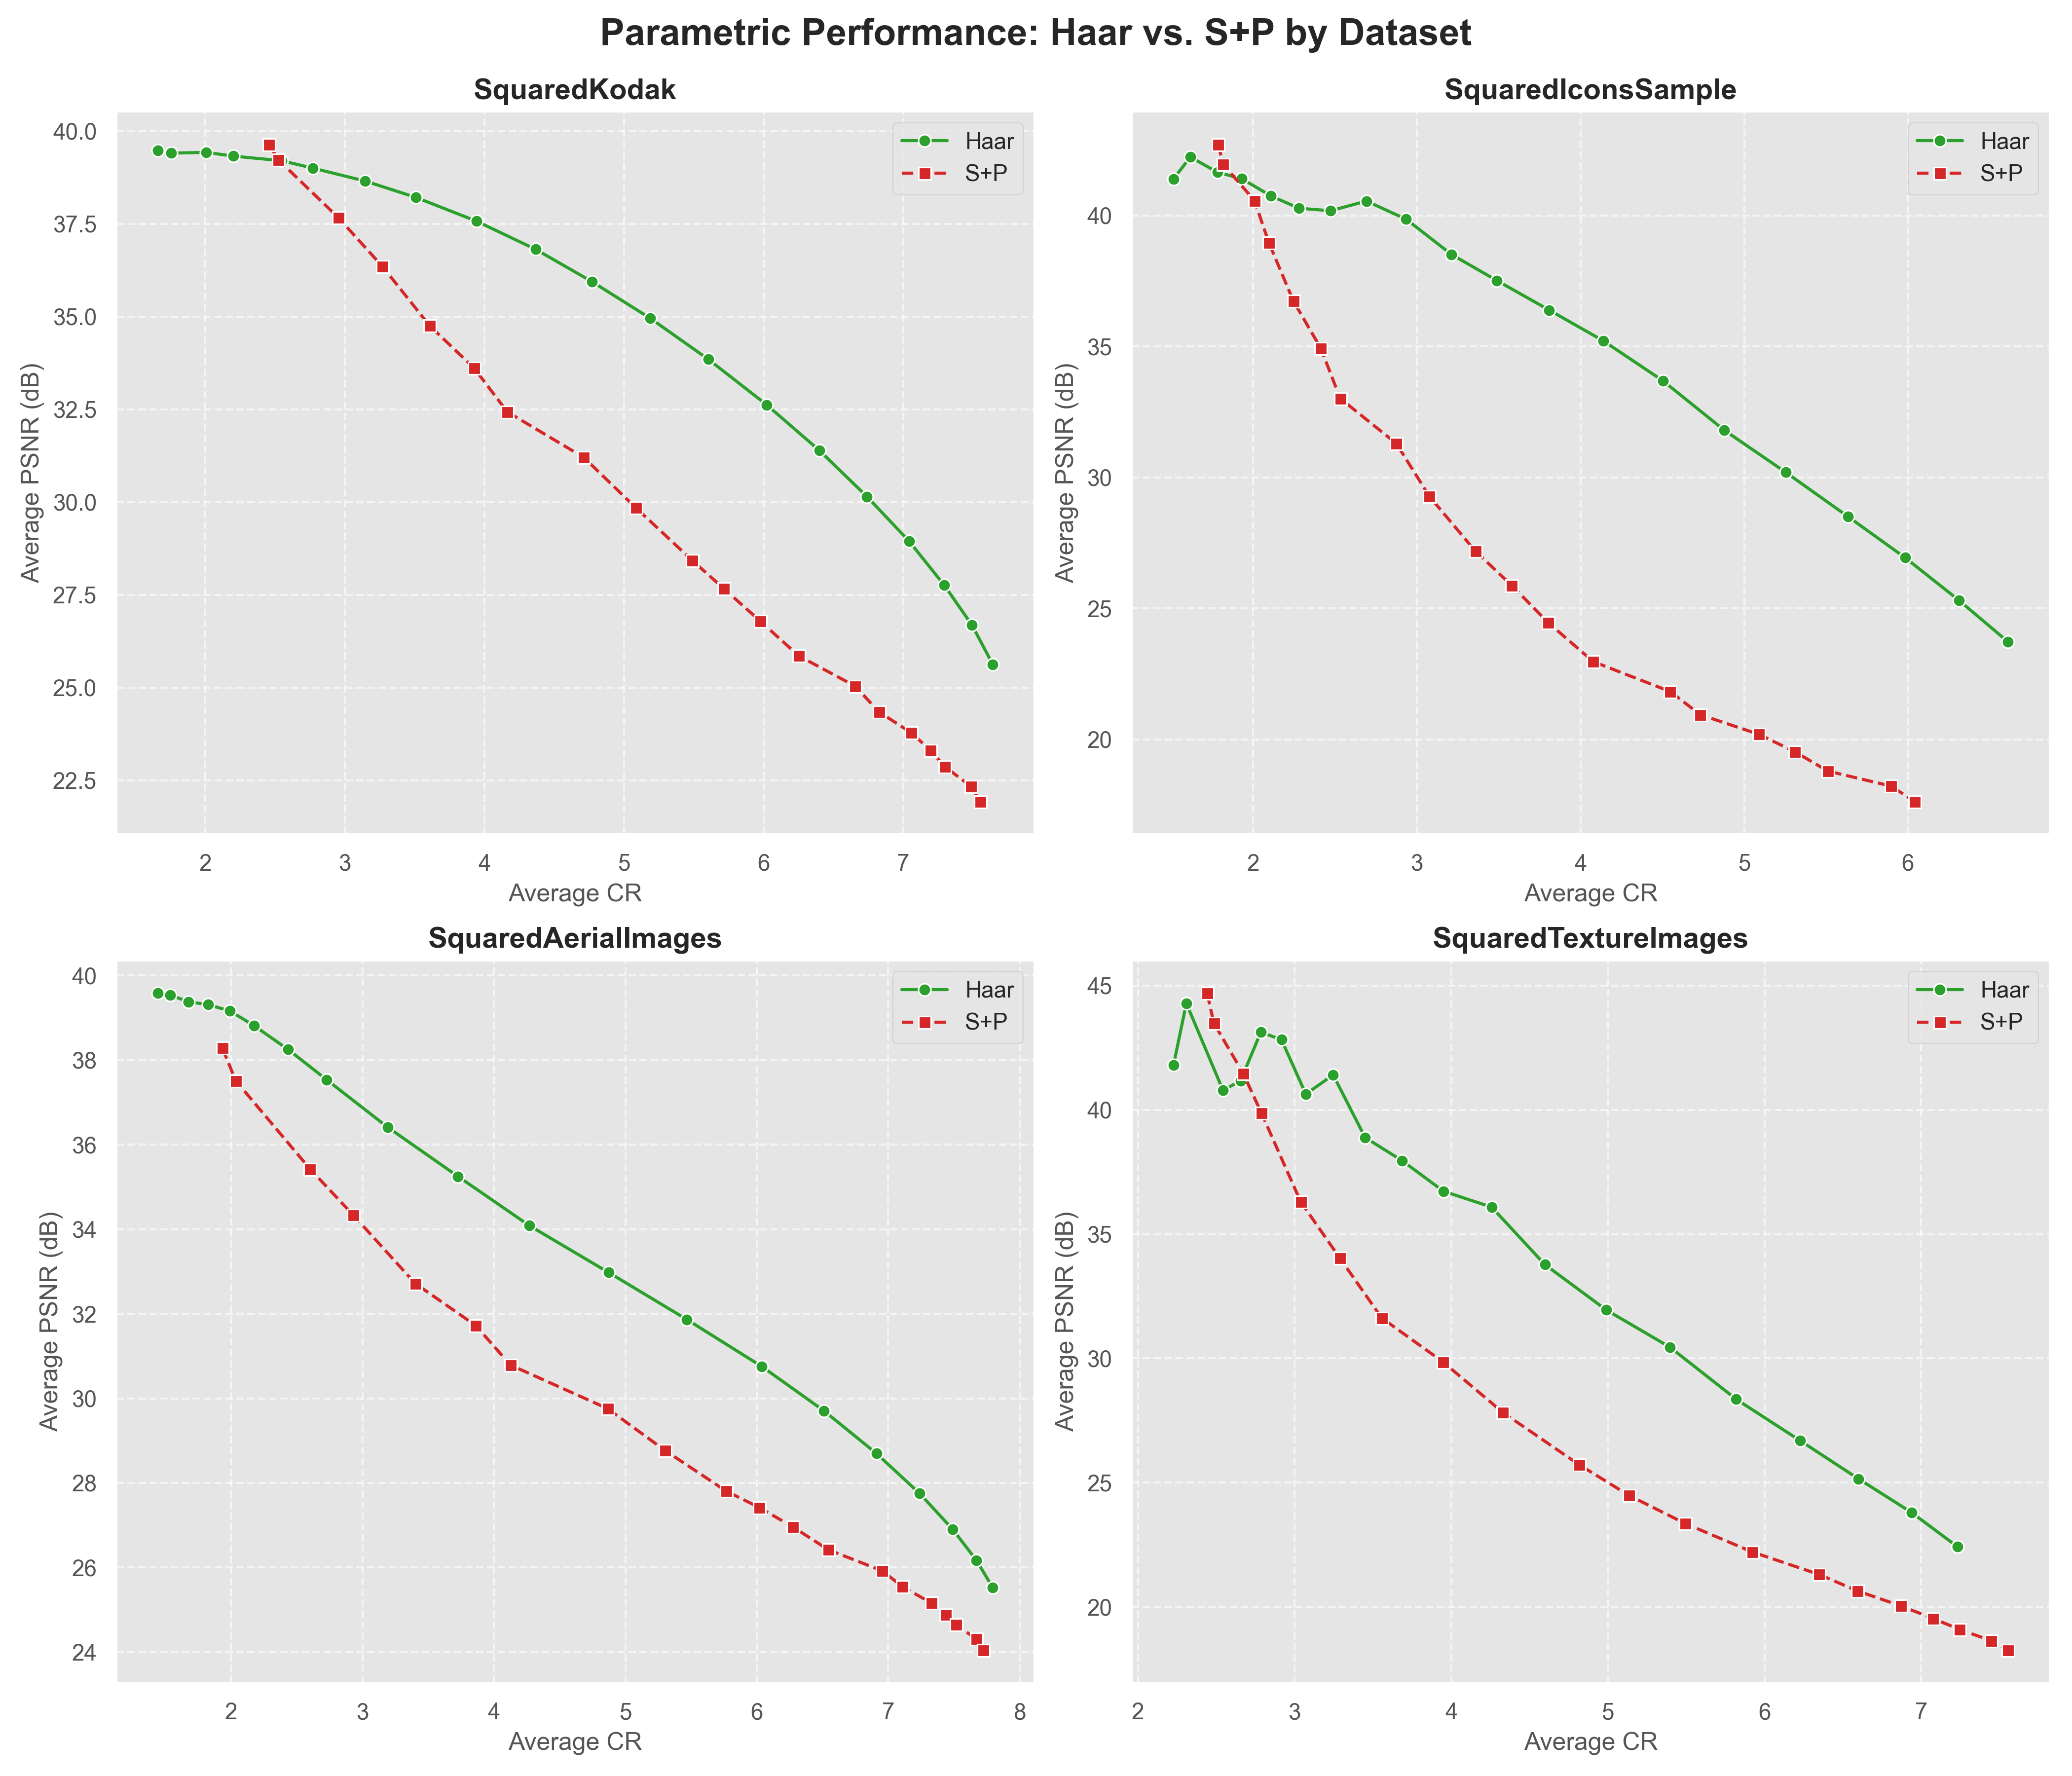
\includegraphics[width=1\linewidth]{results/plots/plot_comparison_Haar_vs_SP_2x2.png}
    \caption{S+P parametric performance: average PSNR vs.\ average compression ratio.}
    \label{fig:haar_vs_sp}
\end{figure}


Fig.~\ref{fig:haar_vs_sp} directly compares Haar and S+P on the same CR--PSNR
axes for each squared dataset. In all four panels, both transforms exhibit the
expected monotone tradeoff between compression ratio and average PSNR, but the
two curves separate as CR increases. For Kodak and AerialImages, the Haar and
S+P curves start close together at low compression ratios (around CR
$\approx 2$ with PSNR near 39–40\,dB), after which the S+P PSNR decreases more
rapidly, yielding several dB lower PSNR than Haar at medium and high CR. A
similar pattern appears for IconsSample and TextureImages: at the lowest CR
values S+P is comparable to Haar (and slightly higher at one operating point
for textures), but beyond roughly CR $\approx 2$ the S+P curve bends downward
more steeply, while the Haar curve remains higher and extends further into the
high-CR regime.


\label{resultssec:SP}

\section{Discussion}
\label{sec:discussion}

\label{discussionsec:Collective}
DCT's superior performance in overall compression is due to the fact that the JPEG Compression Standard has entropy coding algorithms tailor-made to
be effective for quantized DCT. Because of the combination of RLE and heavy quantization of high-frequency components, which results in an abundance of zeroes,
DCT was able to reach much higher compression ratios than other transforms. Of course, without the clever quantization of components less perceptible to humans,
the use of RLE would not be able to reach its full potential. The frequent long runs of zeroes allow many values to be represented by just two. With the Haar and S+P
transforms, a flat predictive encoder was used, which does not decrease the amount of values needed to be represented. Thus, there is a minimum of one bit per value,
whereas in DCT, RLE is able to theoretically break past this minimum because a long run of zeroes is represented with just one value.

DFT, although not as space-efficient when measured against preserving image quality, saw an increase in compression ratio similar
to that of DCT when using JPEG-specified entropy coding techniques, which speaks to its structural similarity to DCT.
The decrease in compression ratio when using a flat linear predictive coder for the Haar and S+P transforms further shows the importance of the structure of
the transform. DPCM and predictive coders heavily rely on correlation between values, which points to the fact that the order in which the values were encoded
with predictive coding after the Haar and S+P transforms were not correlated, causing the two transforms to perform worse in compression ratio when entropy
coding was used.
So, without taking into account the order in which values may be correlated, which is heavily dependent on transform structure, algorithms such as DPCM and predictive
coding may actually decrease compression performance.

By taking advantage of the structure of DCT in the quantization and entropy coding steps, the JPEG Compression Standard performs much better
than the other transforms explored in this project. In the following subsections, we discuss the implications of results for each individual transform.

\label{discussionsec:DWT}
\subsection{Discussion: DWT}
% Content for DWT Discussion subsection
% This file is included in the main conference paper via % Content for DWT Discussion subsection
% This file is included in the main conference paper via % Content for DWT Discussion subsection
% This file is included in the main conference paper via \input{discussion/DWTDiscussion}

As shown in Figure~\ref{fig:dwt_results} in the Results section, the Discrete Wavelet Transform (DWT) using the Haar wavelet basis exhibits degraded performance on the Texture Images and Icons Images datasets as quantization becomes more aggressive. This degradation in performance can be attributed to the finer details present in these datasets, which are more susceptible to being quantized away during the compression process. The quantization step in the compression pipeline tends to discard high-frequency components that represent fine textures and intricate icon details, leading to a more significant loss of visual information in these particular datasets compared to other image types.

The comparison between Haar and DCT on different image types, as shown in Figures~\ref{fig:dwt_aerial} and~\ref{fig:dwt_kodak}, reveals important characteristics of the Haar wavelet transform. Haar performs better on aerial images because it operates on a global image scale, which is particularly effective for aerial images that typically contain large patches of very similar color, such as oceans or deserts. On the other hand, Haar performs worse on Kodak images since it is less optimized than DCT in the JPEG pipeline, as discussed previously. Additionally, Kodak images generally do not contain large global features of the same color as found in aerial images, which limits the effectiveness of Haar's global approach.


As shown in Figure~\ref{fig:dwt_results} in the Results section, the Discrete Wavelet Transform (DWT) using the Haar wavelet basis exhibits degraded performance on the Texture Images and Icons Images datasets as quantization becomes more aggressive. This degradation in performance can be attributed to the finer details present in these datasets, which are more susceptible to being quantized away during the compression process. The quantization step in the compression pipeline tends to discard high-frequency components that represent fine textures and intricate icon details, leading to a more significant loss of visual information in these particular datasets compared to other image types.

The comparison between Haar and DCT on different image types, as shown in Figures~\ref{fig:dwt_aerial} and~\ref{fig:dwt_kodak}, reveals important characteristics of the Haar wavelet transform. Haar performs better on aerial images because it operates on a global image scale, which is particularly effective for aerial images that typically contain large patches of very similar color, such as oceans or deserts. On the other hand, Haar performs worse on Kodak images since it is less optimized than DCT in the JPEG pipeline, as discussed previously. Additionally, Kodak images generally do not contain large global features of the same color as found in aerial images, which limits the effectiveness of Haar's global approach.


As shown in Figure~\ref{fig:dwt_results} in the Results section, the Discrete Wavelet Transform (DWT) using the Haar wavelet basis exhibits degraded performance on the Texture Images and Icons Images datasets as quantization becomes more aggressive. This degradation in performance can be attributed to the finer details present in these datasets, which are more susceptible to being quantized away during the compression process. The quantization step in the compression pipeline tends to discard high-frequency components that represent fine textures and intricate icon details, leading to a more significant loss of visual information in these particular datasets compared to other image types.

The comparison between Haar and DCT on different image types, as shown in Figures~\ref{fig:dwt_aerial} and~\ref{fig:dwt_kodak}, reveals important characteristics of the Haar wavelet transform. Haar performs better on aerial images because it operates on a global image scale, which is particularly effective for aerial images that typically contain large patches of very similar color, such as oceans or deserts. On the other hand, Haar performs worse on Kodak images since it is less optimized than DCT in the JPEG pipeline, as discussed previously. Additionally, Kodak images generally do not contain large global features of the same color as found in aerial images, which limits the effectiveness of Haar's global approach.


\label{discussionsec:sp}
\subsection{Discussion: S+P}
Figs.~\ref{fig:haar_vs_sp} show that, in our current pipeline, the S+P transform does not surpass the Haar wavelet in rate--distortion performance. S+P remains competitive with Haar at very low bit-rates, but its PSNR degrades more quickly as quantization becomes coarser across all datasets. This behavior aligns with several structural differences between the two transforms and with the way our quantizer interacts with their coefficient statistics.

First, S+P modifies the basic Haar lifting step by introducing an in-loop prediction on the highpass branch. After computing the integer lowpass and preliminary detail coefficients $(s, d_1)$, S+P replaces $d_1[l]$ with a residual
\[
d[l] = d_1[l] - 
\left\lfloor 
    \frac{\mathrm{pred}(s, d_1[l+1])}{2^{\text{shift}}}
\right\rfloor,
\]
where $\mathrm{pred}$ is a fixed linear combination of neighboring lowpass differences and the next detail value. This predictor effectively acts as an additional highpass filter: it substantially reduces low-frequency leakage in the detail band whenever the correlation condition $\rho > 1/3$ holds, thereby lowering the variance and first-order entropy of $d[n]$. While this whitening is advantageous at the transform stage, it also concentrates more energy into the highest spatial frequencies, which are precisely the coefficients most heavily attenuated by our coarse scalar quantizer. Moderate step sizes that Haar tolerates well therefore produce noticeably larger PSNR losses under S+P.

Second, unlike Haar, which produces subbands with simple and predictable variance structure, the S+P transform applies additional prediction on the highpass branch. This prediction further suppresses low-frequency leakage in the detail bands, effectively shifting more residual energy toward the highest frequencies. Although this reduces the first-order entropy of the detail coefficients—an advantage for lossless or near-lossless coding—it also increases the sensitivity of these coefficients to coarse scalar quantization, which disproportionately attenuates high-frequency components. Because our quantization parameters were tuned heuristically and not optimized for S+P’s predictor-adjusted subbands, the resulting step sizes do not match the actual coefficient distributions well, contributing to the larger loss in PSNR at matched bit-rates.

Finally, Fig.~\ref{fig:effectEntropyCoding} shows that although S+P achieves some of the highest direct compression ratios before entropy coding, the additional gain from our backend is smaller for S+P than for Haar. Our entropy coder consists of a simple JPEG-style differential predictor followed by symbolwise Huffman coding; it does not perform run-length coding or adaptive context modeling. Because S+P already removes much of the spatial correlation and flattens the coefficient structure, it leaves less residual redundancy for this backend to exploit. Haar, by comparison, retains more correlation patterns that Huffman coding can capitalize on, leading to larger post–entropy-coding improvements.

Taken together, these factors explain why S+P appears promising at the transform stage, with lower entropy and strong direct compression, yet yields a weaker end-to-end CR--PSNR tradeoff than Haar under our current JPEG-style pipeline. With predictor-aware quantization and a more sophisticated entropy model, S+P’s relative position could plausibly change.


\label{discussionsec:fourier}
\subsection{Discussion: DCT + DFT}
We have already established that the DCT outperforms the DFT across all datasets. However, it is worth noting that due to the similar nature of the transforms, their performance is relatively consistent across datasets. In Fig. \ref{fig:dctvsdft}, we can see that they both perform better on the Kodak and Aerial Images datasets, and worse on Textures and Icons. This is consistent with their theory since the images in Textures and Icons are both more likely to have more rapid changes in pixel values corresponding to higher frequency waveforms.

We briefly mentioned in results how some parts of entropy coding like RLE were specifically designed for the DCT. Fig. \ref{fig:dctcrvsdcr} shows the gap between the expected compression ratio based purely on the entropy of the transformed image versus the actual compression ratio achieved. At lower quantization scales, the RLE makes little difference as there are still many nonzero values. However, as quantization is made more aggresive the returns from RLE increase massively as there are longer and longer runs of 0s.



\appendices
\section{Theoretical Foundation for Haar Wavelet Transform}
\label{apx:haartheory}
% Appendix: Detailed Theoretical Foundation for Haar Wavelet Transform
% This file contains the detailed mathematical exposition moved from the main methods section

\paragraph{Vector Spaces and Nested Approximations}

The foundation of wavelet transform can be understood through the definition of a set of nested vector spaces. We can represent any signal as piecewise-constant functions defined on the half-open interval $[0, 1)$. We utilize vector spaces, denoted as $V^j$, to represent these functions at different resolutions.

The space $V^0$ contains functions that are constant over the entire interval $[0, 1)$. A one-pixel image is an element of this space. The space $V^1$ contains functions with two constant pieces over the intervals $[0, 1/2)$ and $[1/2, 1)$. The space $V^2$ contains functions with four constant pieces over the intervals $[0, 1/4)$, $[1/4, 1/2)$, $[1/2, 3/4)$, and $[3/4, 1)$. Generalizing this, the space $V^j$ includes all piecewise-constant functions defined on $[0, 1)$ with constant pieces over each of $2^j$ equal subintervals:
$$ \left[0, \frac{1}{2^j}\right), \left[\frac{1}{2^j}, \frac{2}{2^j}\right), \cdots, \left[\frac{2^j-1}{2^j}, 1\right) $$

A crucial property of these spaces is their nested structure. Because a function that is constant over a large interval is inherently constant over any subdivision of that interval, every vector in $V^j$ is also contained in $V^{j+1}$. For example, a function with two intervals can be described as a function with four intervals where pairs of intervals have identical values. This creates a nested set of spaces:
$$V^0 \subset V^1 \subset V^2 \subset \dots$$

This nested structure is essential for the transform and motivates our representation of signals as this family of vector spaces.

\paragraph{Scaling Functions (The Basis for $V^j$)}

The basis functions for the spaces $V^j$ are known as \textbf{scaling functions}, usually denoted by $\phi$. A natural and simple basis for $V^j$ is derived from the scaled and translated "box" function $\phi(x)$, defined as:
$$\phi(x) := \begin{cases} 1 & \text{for } 0 \le x < 1 \\ 0 & \text{otherwise} \end{cases}$$

For a specific resolution level $j$, the basis functions $\phi_i^j$ are defined by scaling and translating $\phi(x)$:
$$\phi_i^j(x) := \phi(2^j x - i), \quad i = 0, \dots, 2^j - 1$$

A visualization for this basis in $V^3$ is shown in Figure~\ref{fig:basis_functions}(a).

\paragraph{Inner Products and Orthogonality}

To define wavelets, we must first define an \textbf{inner product} to measure the relationship between functions. The standard inner product for two elements $f, g \in V^j$ is defined as:
$$\langle f|g\rangle := \int_{0}^{1}f(x)g(x)dx$$

Using this inner product, we define a new vector space \textbf{$W^j$} as the \textbf{orthogonal complement} of $V^j$ in $V^{j+1}$. In other words, we will let $W^j$ be the space of all functions in $V^{j+1}$ that are orthogonal to all functions in $V^j$ under the chosen inner product. Informally, we can think of the wavelets in $W^j$ as a means for representing the parts of a function in $V^{j+1}$ that cannot be represented in $V^j$.

A collection of linearly independent functions $\psi_i^j(x)$ spanning $W^j$ are called \textbf{wavelets}. These basis functions have two important properties:
\begin{enumerate}
\item The basis functions $\psi_i^j$ of $W^j$, together with the basis functions $\phi_i^j$ of $V^j$, form a basis for $V^{j+1}$.
\item Every basis function $\psi_i^j$ of $W^j$ is orthogonal to every basis function $\phi_i^j$ of $V^j$ under the chosen inner product.
\end{enumerate}

Thus, the "detail coefficients" are really coefficients of the wavelet basis functions.

\paragraph{The Haar Wavelet Basis Functions}

The wavelets corresponding to the box basis are called \textbf{Haar wavelets}. The "mother wavelet" $\psi(x)$ is defined as:
$$\psi(x) := \begin{cases} 1 & \text{for } 0 \le x < 1/2 \\ -1 & \text{for } 1/2 \le x < 1 \\ 0 & \text{otherwise} \end{cases}$$

Similar to the scaling functions, the Haar wavelets for a specific level $j$ are generated by scaling and translating this function:
$$\psi_i^j(x) := \psi(2^j x - i), \quad i = 0, \dots, 2^j - 1$$

Figure~\ref{fig:basis_functions}(b) illustrates the relationship between the scaling functions (blue) and the Haar wavelet basis functions (red) for $W^2$. The wavelets capture the detail information that cannot be represented in the lower-resolution space $V^2$.

\paragraph{Generalizing to Other Basis}

This illustration of this specific vector space of piecewise constant functions is unique to the Haar Wavelets,
however we can similarly define other vector spaces and inner products to work with different wavelets. The essential part illustrated by Haar is that the vector spaces must be nested and the definition of the wavelet space as the orthogonal complement of the scaling functions inside the next resolution level. This general idea of energy compactation into the lower resolution's basis and using the wavelets as the detail coefficient remain the same regardless of the basis. Figure~\ref{fig:spline_bases} demonstrates alternative wavelet bases using linear and quadratic splines.

\begin{figure}[ht]
  \centering
  \begin{minipage}{0.24\textwidth}
    \centering
    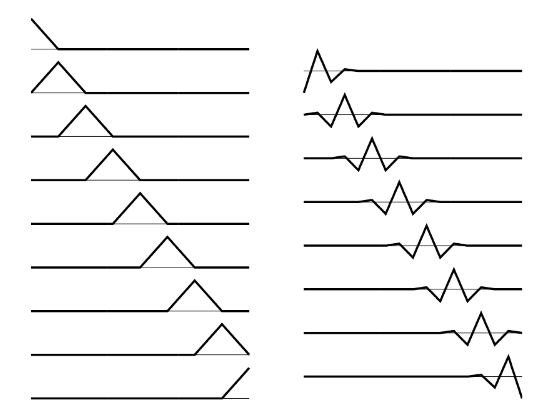
\includegraphics[width=\textwidth]{methods/DWTdiagrams/linear_spline_basis.png}
    \subcaption{Linear B-spline scaling and corresponding wavelet functions}
  \end{minipage}
  \hfill
  \begin{minipage}{0.24\textwidth}
    \centering
    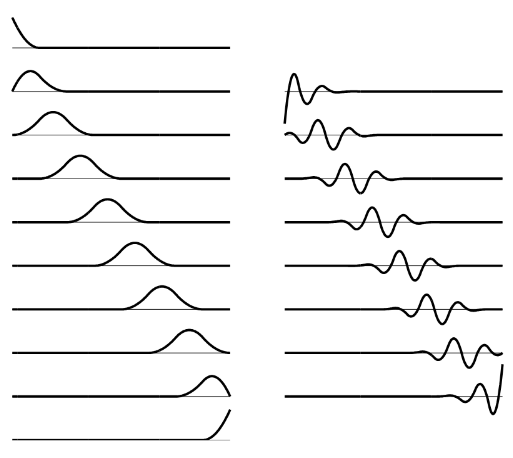
\includegraphics[width=\textwidth]{methods/DWTdiagrams/quadratic_spline_basos.png}
    \subcaption{Quadratic B-spline scaling and corresponding wavelet functions}
  \end{minipage}
  \caption{Alternative wavelet bases demonstrating different spline functions: linear and quadratic splines, showing alternatives to the Haar wavelets. Figures adapted from \cite{stollnitz_wavelet_2}}.
  \label{fig:spline_bases}
\end{figure}

It is somewhat standard to treat the space as some space of functions from the half open interval $[0, 1)$ when dealing with images because we can use the standard inner product previously defined very effectively but there is nothing that strictly requires such representation.

\section{The ``Correlation $> 1/3$'' Condition in Haar and S+P}

Many analyses of the Haar and S+P transforms rely on the assumption that adjacent samples in natural images exhibit a positive correlation greater than $1/3$. This condition arises from a simple variance calculation of the Haar lifting step.

Let $c[n]$ be a stationary one-dimensional signal with variance $\sigma^2$ and correlation coefficient
\[
\rho \;=\; \frac{\mathrm{Covar}(c[n],\,c[n+1])}{\sigma^2}.
\]

In the $1$D Haar transform, each pair $(c[2n],\,c[2n+1])$ is mapped to an average and a difference:
\[
s[n] = \frac{c[2n] + c[2n+1]}{2}, \qquad
d_1[n] = c[2n+1] - c[2n].
\]

Assuming stationarity, the variances of these components are:
\[
\mathrm{Var}(s) = \frac{\sigma^2}{2}\,(1 + \rho),
\qquad
\mathrm{Var}(d_1) = 2\sigma^2\,(1 - \rho).
\]

For the transform to be variance-reducing (or at least not variance-increasing), we require that the total output variance not exceed the original variance of the pair:
\[
\mathrm{Var}(s) + \mathrm{Var}(d_1) \;\le\; 2\sigma^2.
\]

Substituting the expressions above yields
\[
\frac{\sigma^2}{2}(1 + \rho) + 2\sigma^2(1 - \rho)
\;\le\;
2\sigma^2,
\]
which simplifies to
\[
\rho \;>\; \frac{1}{3}.
\]

Thus, when the correlation between neighboring samples exceeds $1/3$, the Haar averaging--differencing step reduces redundancy by lowering total variance. Since natural images typically exhibit correlations in the range $0.8$--$0.95$, this condition is amply satisfied in practice, explaining the effectiveness of Haar-based and S+P transforms for decorrelation and compression.

\section{S+P Frequency domain interpretation}
Although the S+P transform is defined via local integer operations, its behavior is illuminating when viewed in the frequency domain. If we ignore truncation for the sake of analysis and treat the operations as linear, the mapping from the original sequence $c[n]$ to the highpass residual $d[n]$ can be represented as a linear time-invariant filter with a frequency response $F(\mathrm{e}^{j\omega})$.

The S stage alone already suppresses low frequencies in the highpass band, but it does so relatively mildly; the resulting highpass spectrum still exhibits considerable low-frequency energy due to the piecewise-constant nature of the Haar-like filter. By embedding prediction in the transform, S+P effectively implements an additional highpass filter: the predictor attempts to explain away low-frequency variations in $d_1[n]$ using neighboring lowpass differences and adjacent highpass values. When the predictor coefficients are chosen appropriately, $|F(\mathrm{e}^{j\omega})|$ exhibits significantly stronger attenuation at low frequencies than the basic S transform.

There is, of course, a trade-off. Stronger low-frequency attenuation generally comes at the cost of some amplification in higher frequencies. For smooth, low-noise images, this trade-off is supposedly advantageous: the additional whitening reduces the variance and first-order entropy of $d[n]$, improving compressibility. For highly textured or noisy images, it may be beneficial to temper the predictor so as not to over-amplify high-frequency content. Said and Pearlman demonstrate that, in practice, a small set of carefully tuned predictors can work well across a broad range of natural and medical images~[9]. 
\section{The Fast Fourier Transform}
\label{apx:fft}
As discussed in Section \ref{methodsec:fourier}, a naive DFT implementation has a runtime of $\mathcal{O}(N^2)$ for an input signal $x=\{x_0,\dots,x_{N-1}\}$. The Fast Fourier Transform (FFT) significantly speeds up this process. The name ``FFT" actually refers to a whole family of algorithms that can solve a wider range of problems, but all of them take advantage of the symmetry in the complex plane to use a divide and conquer scheme. The FFT was first formally proposed by Cooley and Tukey in their 1965 paper \cite{CooleyTukey}, and the mathematical discussion here is inspired by Broughton \cite{broughton2009discrete}. We start with Equation \ref{eq:dfttransform} for the DFT Transform, but instead write it as 
\begin{equation}
    X_{(N/2)k_1+k_0}=\sum_{m=0}^{N-1}x_m(-1)^{k_1m}e^{-2\pi ik_0/N},\label{eq:fftstart}
\end{equation}
where $k_1\in\{0,1\}$ and $0\leq k_2<N/2$. Note that now when $k_1=0$ we are referring to the first $N/2$ coefficients, while when $k_1=1$ we are referring to the second half. If we then split the sum into its even and odd terms and simplify, we get that 
\begin{equation}
    X_{k_0}=F_1(k_0)+e^{-2\pi ik_0/N}F_2(k_0)\label{eq:fftrelation1}
\end{equation}
and
\begin{equation}
    X_{N/2+k_0}=F_1(k_0)-e^{-2\pi ik_0/N}F_2(k_0),\label{eq:fftrelation2}
\end{equation}
where 
\begin{equation}
    F_1(k_0)=\sum_{m=0}^{N-1}x_{2m}e^{-2\pi ik_0/(N/2)}\label{eq:evenfft}
\end{equation}
and 
\begin{equation}
    F_2(k_0)=\sum_{m=0}^{N-1}x_{2m+1}e^{-2\pi ik_0/(N/2)}.\label{eq:oddfft}
\end{equation}
Note that $F_1(k_0)$ and $F_2(k_0)$ describe the DFT on the even and odd terms of the original signal $x$, respectively. In other words, to get the full length $N$ DFT, one needs only to calculate the length $N/2$ DFT on the even and odd terms, then sum them to get the first $N/2$ terms for the full DFT (Eq. \ref{eq:fftrelation1}) and take their difference for the second $N/2$ terms (Eq. \ref{eq:fftrelation2}). This process can then be repeated recursively, further breaking down each half transform. The first step of this process is shown in Fig. \ref{fig:FFTalgorithm}. In this sense, the FFT is a classic divide and conquer algorithm, and an application of the Master Theorem can rigorously prove the $\mathcal{O}(N\log N)$ runtime that results. We refer a reader interested in the derivations of the relations in Equation \ref{eq:fftrelation1} and Equation \ref{eq:fftrelation2} once again to Broughton \cite{broughton2009discrete}. For an in-depth walkthrough of how the FFT can be implemented efficiently, see the CP algorithms page \cite{CPAFFT}.

\begin{figure}[ht]
    \centering
    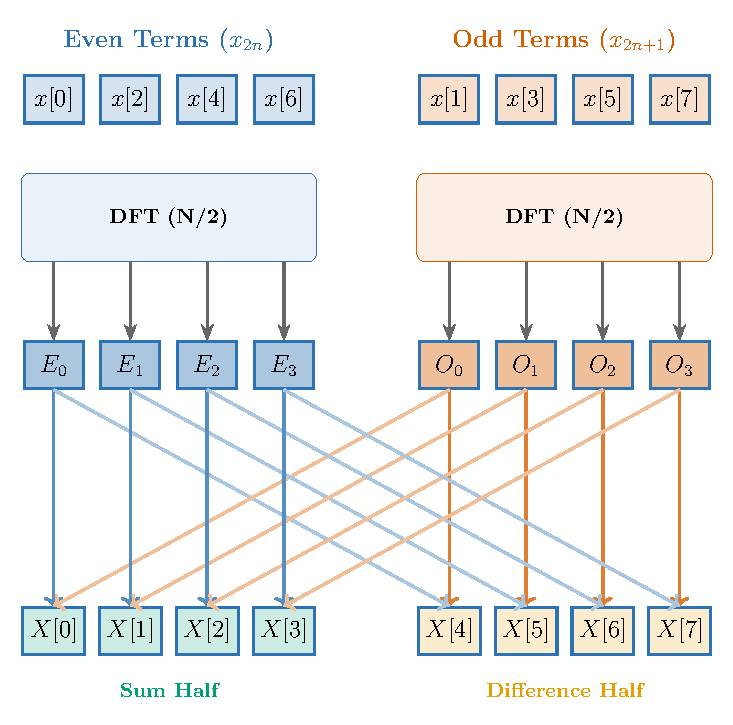
\includegraphics[width=1\linewidth]{methods/Fourierdiagrams/fft.pdf}
    \caption{The first recursive step in the FFT.}
    \label{fig:FFTalgorithm}
\end{figure}

\section*{Acknowledgment}
We would like to thank our advisor Layla Oesper for all her help throughout this project.

\begin{thebibliography}{00}

\bibitem{BoumanJPEGLab} 
C. A. Bouman, ``JPEG Image Coding Laboratory Manual,'' \emph{Purdue University} Available: https://engineering.purdue.edu/~bouman/grad-labs/JPEG-Image-Coding/pdf/lab.pdf.

\bibitem{CPAFFT} 
CP-Algorithms contributors, ``Fast Fourier Transform (FFT),'' \emph{CP-Algorithms}. Available: https://cp-algorithms.com/algebra/fft.html.

\bibitem{CooleyTukey} 
J. W. Cooley and J. W. Tukey, ``An Algorithm for the Machine Calculation of Complex Fourier Series,'' \emph{Mathematics of Computation}, vol. 19, no. 90, pp. 297--301, 1965.

\bibitem{broughton2009discrete} 
S. A. Broughton and K. Bryan, \emph{Discrete Fourier Analysis and Wavelets: Applications to Signal and Image Processing}. Hoboken, NJ: John Wiley \& Sons, 2009.

\bibitem{chlubna_comparative_2025} 
T. Chlubna and P. Zemčík, ``Comparative survey of image compression methods across different pixel formats and bit depths,'' \emph{Signal, Image and Video Processing}, vol. 19, no. 12, p. 981, Sep. 2025.

\bibitem{devore_image_1992} 
R. A. DeVore, B. Jawerth, and B. J. Lucier, ``Image compression through wavelet transform coding,'' \emph{IEEE Transactions on Information Theory}, vol. 38, no. 2, pp. 719--746, Mar. 1992.

\bibitem{han_technical_2021} 
J. Han \emph{et al.}, ``A Technical Overview of AV1,'' \emph{Proceedings of the IEEE}, vol. 109, no. 9, pp. 1435--1462, Sept. 2021.

\bibitem{ibraheem_comprehensive_nodate} 
M. K. Ibraheem, ``A Comprehensive Literature Review on Image and Video Compression: Trends, Algorithms, and Techniques,'' \emph{IIETA}. [Online]. Available: https://iieta.org/journals/isi/paper/10.18280/isi.290307.

\bibitem{jayasankar_survey_2021} 
U. Jayasankar, V. Thirumal, and D. Ponnurangam, ``A survey on data compression techniques: From the perspective of data quality, coding schemes, data type and applications,'' \emph{Journal of King Saud University - Computer and Information Sciences}, vol. 33, no. 2, pp. 119--140, Feb. 2021.

\bibitem{khayam_discrete_2003} 
S. A. Khayam, ``The discrete cosine transform (DCT): theory and application,'' \emph{Michigan State University}, vol. 114, no. 1, p. 31, 2003.

\bibitem{lee_end--end_2020} 
J. Lee, S. Cho, and M. Kim, ``An End-to-End Joint Learning Scheme of Image Compression and Quality Enhancement with Improved Entropy Minimization,'' \emph{arXiv preprint arXiv:1912.12817}, Mar. 2020.

\bibitem{mali_neural_2022} 
A. Mali, A. Ororbia, D. Kifer, and L. Giles, ``Neural JPEG: End-to-End Image Compression Leveraging a Standard JPEG Encoder-Decoder,'' \emph{arXiv preprint arXiv:2201.11795}, Jan. 2022.

\bibitem{mallat2009wavelet} 
S. Mallat, \emph{A Wavelet Tour of Signal Processing: The Sparse Way}, 3rd ed. Academic Press, 2009.

\bibitem{rad_predictive_2013} 
R. M. Rad, A. Attar, and A. Shahbahrami, ``A predictive algorithm for multimedia data compression,'' \emph{Multimedia Systems}, vol. 19, no. 2, pp. 103--115, Mar. 2013.

\bibitem{raid_jpeg_2014} 
A. M. Raid, W. M. Khedr, M. A. El-dosuky, and W. Ahmed, ``Jpeg Image Compression Using Discrete Cosine Transform - A Survey,'' \emph{arXiv preprint arXiv:1405.6147}, May 2014.

\bibitem{rd_development_2025} 
S. R. D. Sivakumar, ``Development of a Modified Predictive Coding Algorithm for High-Resolution Image Compression in Real-Time Structural Health Monitoring of Metallic Component,'' \emph{Metallurgical and Materials Engineering}, vol. 31, no. 4, pp. 76--83, Apr. 2025.

\bibitem{said1993sp} 
A. Said and W. A. Pearlman, ``Reversible image compression via multiresolution representation and predictive coding,'' \emph{Visual Communications and Image Processing '93}, pp. 664--674, 1993.

\bibitem{said_reversible_1993} 
A. Said and W. A. Pearlman, ``Reversible image compression via multiresolution representation and predictive coding,'' in \emph{Visual Communications and Image Processing '93}, vol. 2094. SPIE, Oct. 1993, pp. 664--674.

\bibitem{sayood_introduction_2012} 
K. Sayood, \emph{Introduction to Data Compression}, 4th ed. Elsevier, 2012.

\bibitem{shannon} 
C. E. Shannon, ``A Mathematical Theory of Communication,'' \emph{The Bell System Technical Journal}, vol. 27, pp. 379--423, 1948.

\bibitem{skodras_discrete_2003} 
A. Skodras, \emph{Discrete Wavelet Transform: An Introduction}. Jan. 2003.

\bibitem{stollnitz_wavelet_1}
D. H. Salesin, T. D. DeRose and E. J. Stollnitz, \emph{Wavelets for Computer Graphics: A Primer, Part 1} in \emph{IEEE Computer Graphics and Applications}, vol. 15, no. 03, pp. 76-84, May 1995.

\bibitem{stollnitz_wavelet_2}
D. H. Salesin, T. D. DeRose and E. J. Stollnitz, \emph{Wavelets for Computer Graphics: A Primer, Part 2} in \emph{IEEE Computer Graphics and Applications}, vol. 15, no. 04, pp. 75-85, July 1995.

\bibitem{wallace_jpeg_1992} 
G. K. Wallace, ``The JPEG Still Picture Compression Standard,'' \emph{IEEE Transactions on Consumer Electronics}, vol. 38, no. 1, Feb. 1992.

\bibitem{weinberger_loco-i_2000} 
M. J. Weinberger, G. Seroussi, and G. Sapiro, ``The LOCO-I lossless image compression algorithm: Principles and standardization into JPEG-LS,'' \emph{IEEE Transactions on Image Processing}, vol. 9, no. 8, pp. 1309--1324, Aug. 2000.

\end{thebibliography}

\end{document}